\chapter{Resultados}
\label{ch:resultados}

Este capítulo presenta los resultados. En lugar de limitarse a presentar cifras en tablas, se procura explicar qué significan y qué hay detrás de cada resultado. Se incluyen numerosas figuras ---aproximadamente cuarenta--- ya que la representación visual aporta una perspectiva complementaria a las tablas numéricas.

%% ============================================================
%% EXPERIMENTO A: COMPARACIÓN DE MODELOS
%% ============================================================

\section{Comparación de modelos (h=7)}

La primera pregunta, y la más obvia: ¿qué modelo reduce más el error? Para averiguarlo se ejecutó cada modelo sobre los tres activos con horizonte de 7 días y doce iteraciones de walk-forward.

\subsection{Los números clave}

La Tabla~\ref{tab:experiment_a} resume los resultados en términos de MAPE ---el error porcentual medio---. En este experimento se utiliza el set completo de variables, incluido el sentimiento.

\begin{table}[H]
\centering
\caption{MAPE (\%) por modelo y activo}
\label{tab:experiment_a}
\begin{tabular}{l|ccc|c}
\hline
\textbf{Modelo} & \textbf{BTC-USD} & \textbf{TSLA} & \textbf{NVDA} & \textbf{Media} \\
\hline
Naive & \textbf{6.04} & 8.32 & 6.66 & 7.01 \\
ARIMA & 6.08 & \textbf{8.29} & \textbf{6.61} & \textbf{6.99} \\
Random Forest & 7.82 & 9.03 & 6.94 & 7.93 \\
XGBoost & 8.49 & 9.09 & 7.02 & 8.20 \\
CNN & 13.15 & 12.48 & 11.79 & 12.47 \\
LSTM & 11.98 & 11.00 & 10.72 & 11.23 \\
GRU & 10.13 & 9.56 & 9.36 & 9.68 \\
\hline
\end{tabular}
\end{table}

El resultado más destacado es que, con este protocolo, \textbf{los baselines ganan}. \textbf{ARIMA} logra el mejor MAPE medio y \textbf{Naive} obtiene resultados muy próximos; activo por activo, Naive lidera en BTC-USD y ARIMA en TSLA y NVDA. Random Forest y XGBoost no mejoran a esos baselines, y en BTC-USD la diferencia es llamativa. Las arquitecturas de deep learning (CNN, LSTM, GRU) quedan claramente atrás en los tres activos. Este resultado, aunque pueda parecer inesperado, no es infrecuente: con series muy ruidosas y señales agregadas, añadir complejidad no siempre compensa.

Más allá del ranking, la distancia entre modelos es importante. En varios casos las diferencias son pequeñas, lo que sugiere que la serie tiene mucho ruido y que una mejora puntual puede no ser estable. Por eso, además del MAPE medio, conviene mirar la dispersión y la consistencia por fold.

\subsection{Bitcoin: el baseline resiste}

Las Figuras~\ref{fig:model_btc_mape} y \ref{fig:model_btc_rmse} muestran los resultados visuales para Bitcoin.

\begin{figure}[H]
\centering
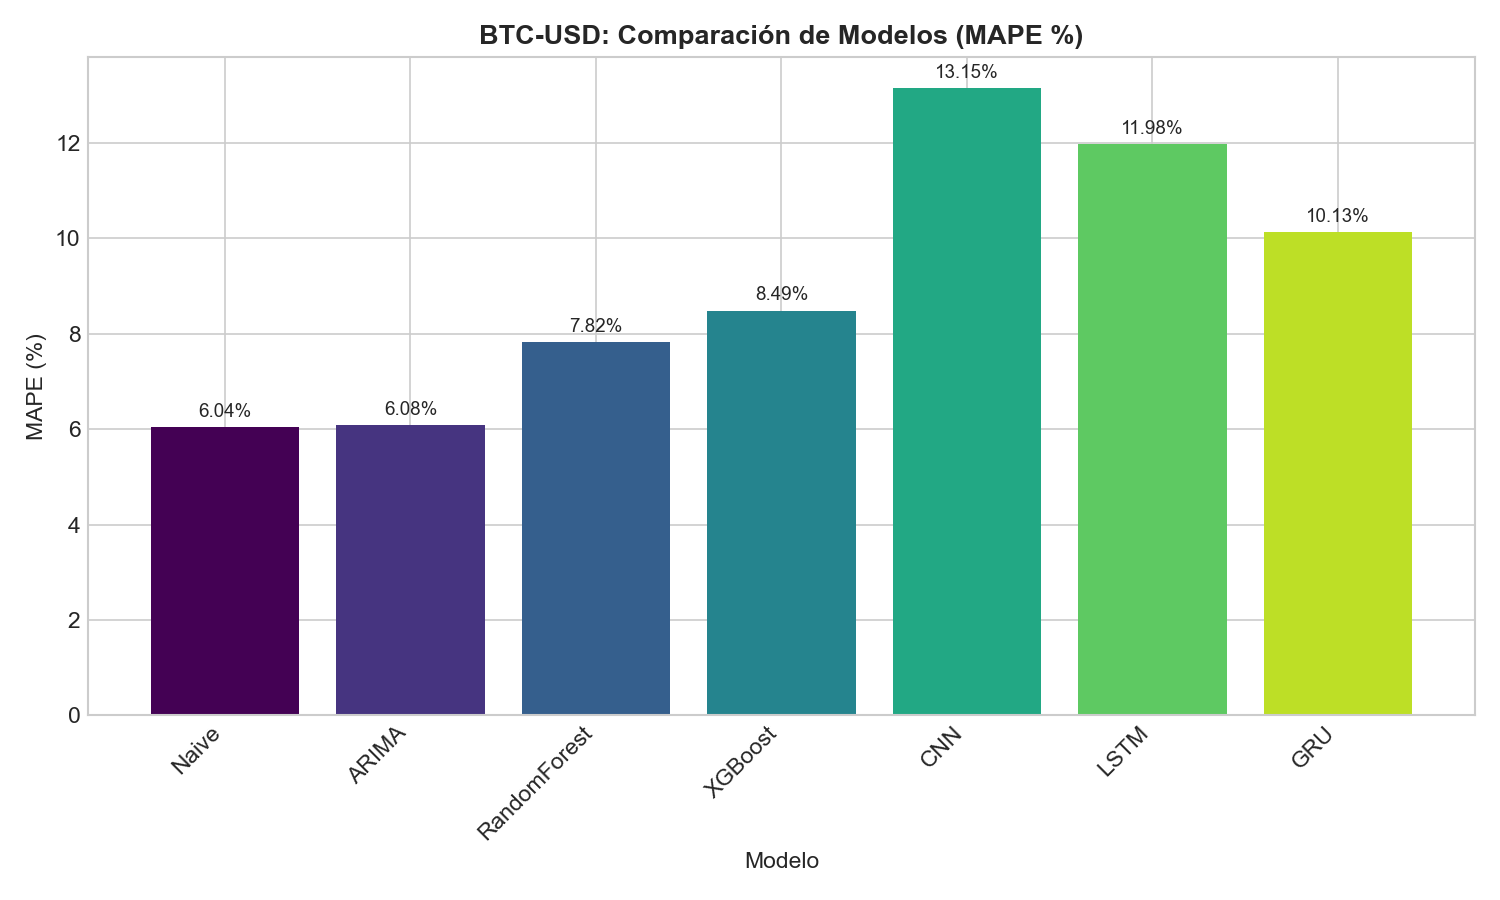
\includegraphics[width=0.95\textwidth]{Imagenes/model_comparison_BTC_USD_mape.png}
\caption{BTC-USD: Comparación de modelos (MAPE \%).}
\label{fig:model_btc_mape}
\end{figure}

\begin{figure}[H]
\centering
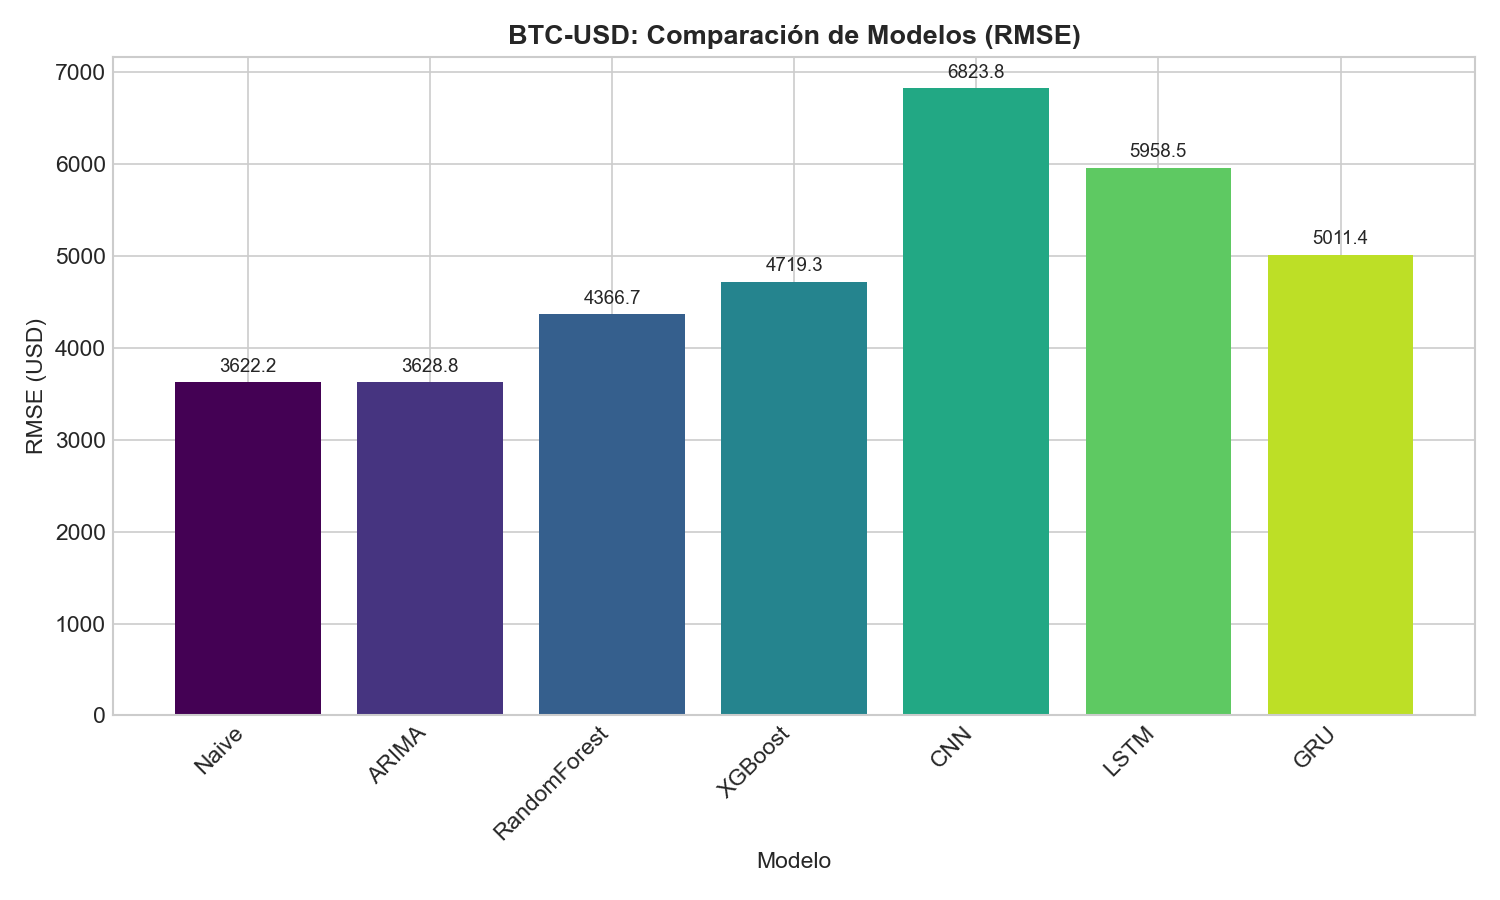
\includegraphics[width=0.95\textwidth]{Imagenes/model_comparison_BTC_USD_rmse.png}
\caption{BTC-USD: Comparación de modelos (RMSE en USD).}
\label{fig:model_btc_rmse}
\end{figure}

En Bitcoin, Naive obtiene el mejor MAPE y ARIMA le sigue de cerca. Los modelos de árboles no solo no mejoran, sino que empeoran de forma apreciable (XGBoost especialmente). Las redes profundas quedan aún más lejos: GRU es la que presenta menor error dentro de las arquitecturas DL, pero incluso esta se aleja de forma notable de los baselines.

La lectura práctica es que Bitcoin sigue siendo un activo difícil para los modelos predictivos. Su volatilidad es tan elevada que un baseline trivial como ``mañana valdrá lo mismo que hoy'' ya es difícil de mejorar. Si ni siquiera añadir indicadores técnicos y sentimiento basta para superar al Naive, es que la señal disponible no compensa el ruido.

\subsection{Tesla: ARIMA toma ventaja}

Las Figuras~\ref{fig:model_tsla_mape} y \ref{fig:model_tsla_rmse} muestran los resultados para Tesla.

\begin{figure}[H]
\centering
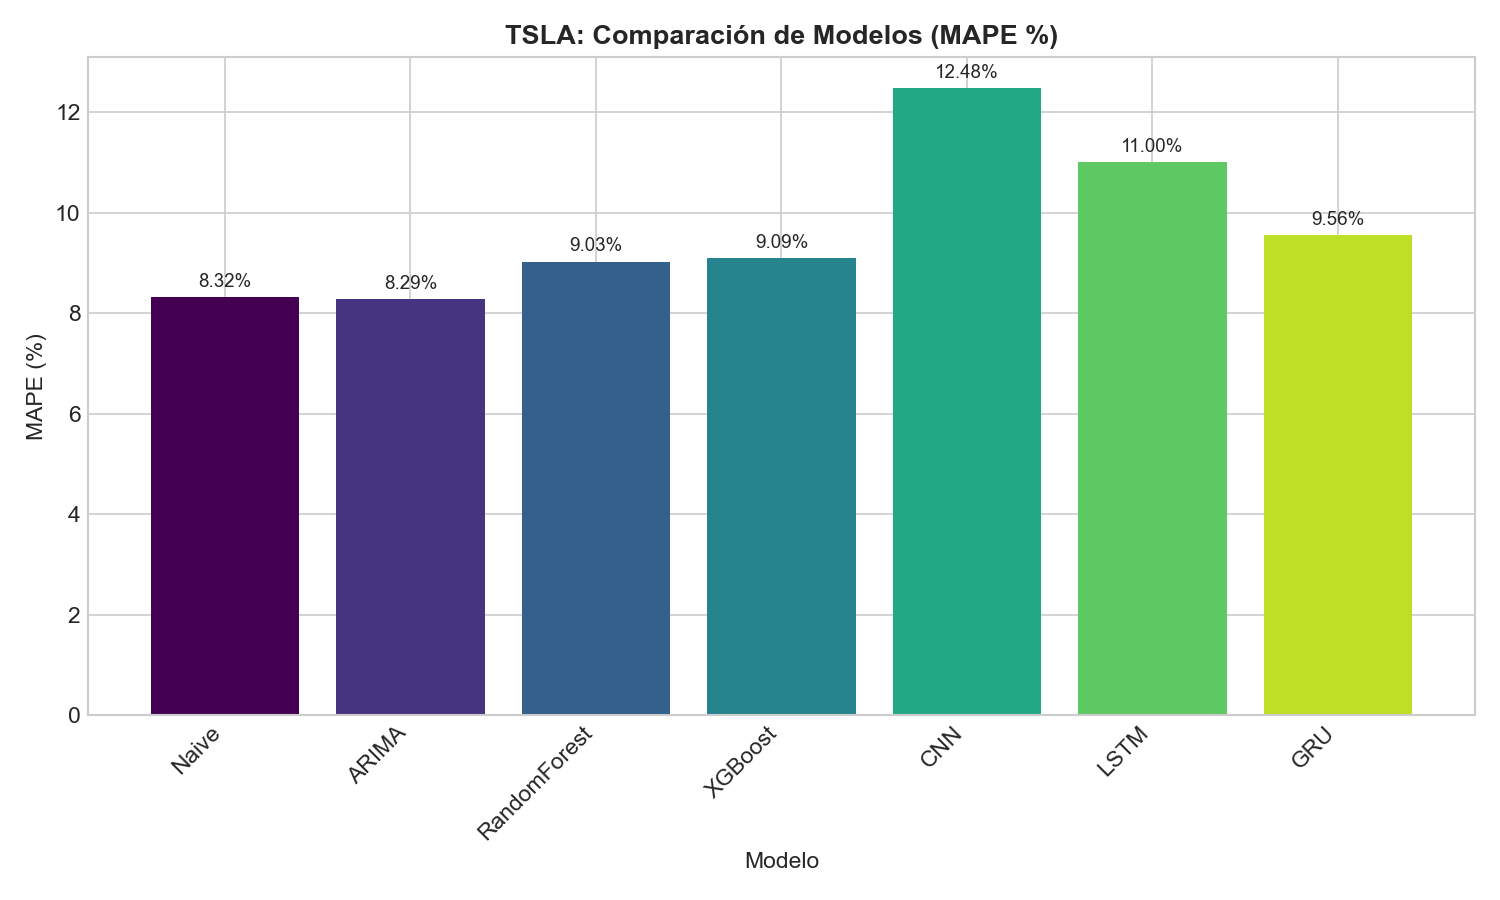
\includegraphics[width=0.95\textwidth]{Imagenes/model_comparison_TSLA_mape.png}
\caption{TSLA: Comparación de modelos (MAPE \%).}
\label{fig:model_tsla_mape}
\end{figure}

\begin{figure}[H]
\centering
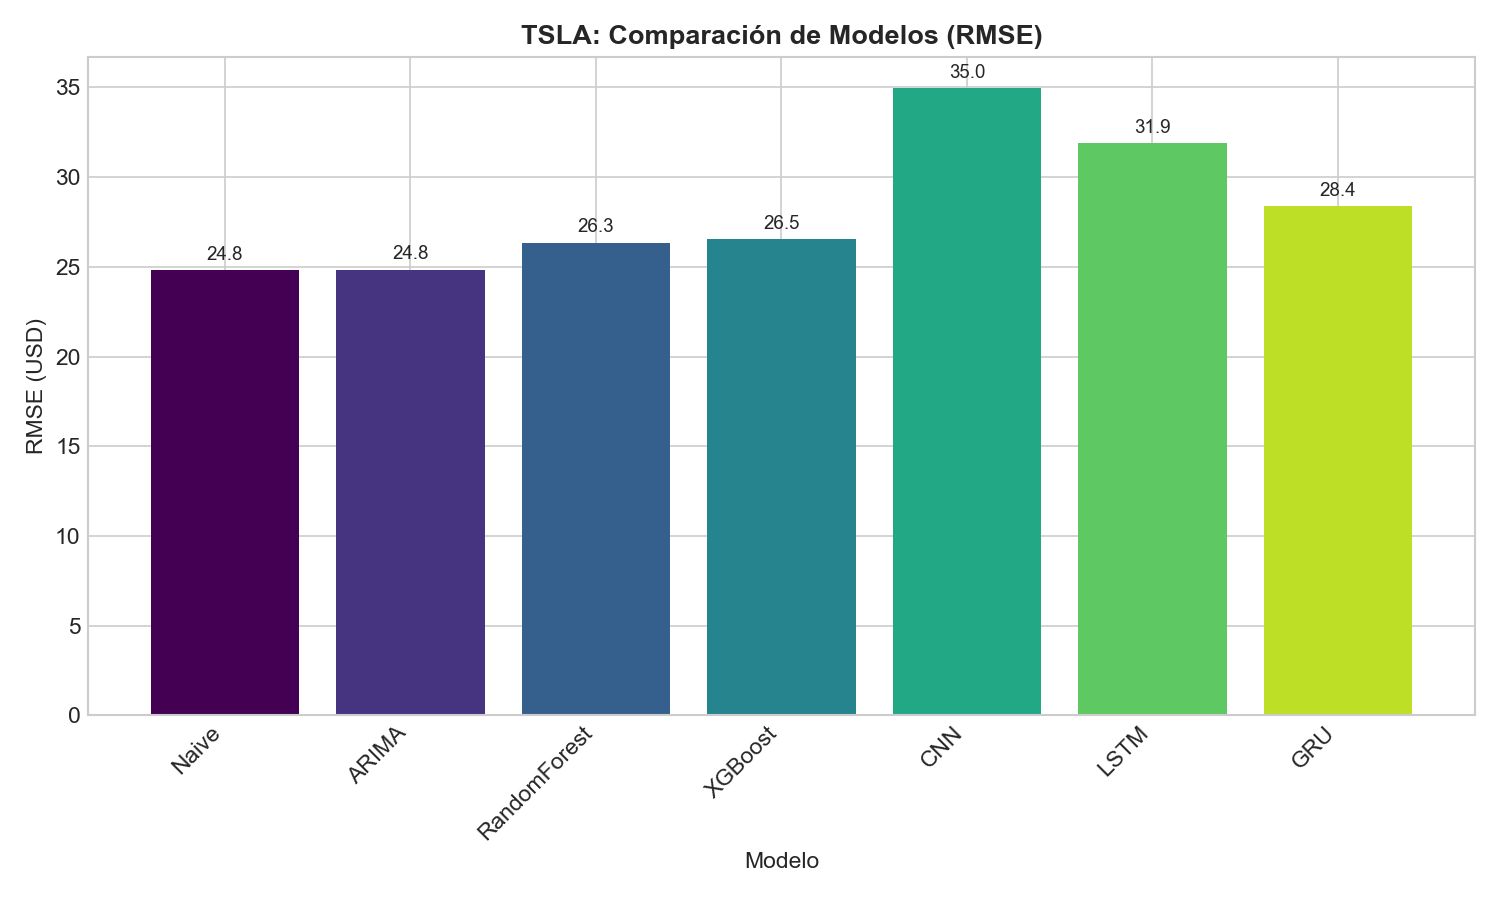
\includegraphics[width=0.95\textwidth]{Imagenes/model_comparison_TSLA_rmse.png}
\caption{TSLA: Comparación de modelos (RMSE en USD).}
\label{fig:model_tsla_rmse}
\end{figure}

En Tesla, ARIMA pasa a ser el mejor en MAPE y Naive queda prácticamente empatado. Los modelos de árboles no superan a los baselines y quedan por encima, aunque la diferencia es menor que en BTC-USD. Las redes profundas no resultan competitivas en esta configuración experimental: GRU es el modelo con menor error dentro de DL, pero aun así queda por encima de Naive/ARIMA, y CNN es la que más se degrada. Esto sugiere que, con series con cambios de régimen, aumentar la complejidad sin un tuning cuidadoso puede empeorar la generalización.

El rendimiento de Random Forest y XGBoost es razonable pero no aporta ventaja clara con retardos simples. Una ingeniería de características más rica (o modelos diseñados específicamente para forecasting tabular) podría mejorar su posición, pero en este trabajo se priorizó la comparativa entre familias de modelos sin optimización exhaustiva.

\subsection{Nvidia: ARIMA destaca}

Las Figuras~\ref{fig:model_nvda_mape} y \ref{fig:model_nvda_rmse} muestran los resultados para Nvidia.

\begin{figure}[H]
\centering
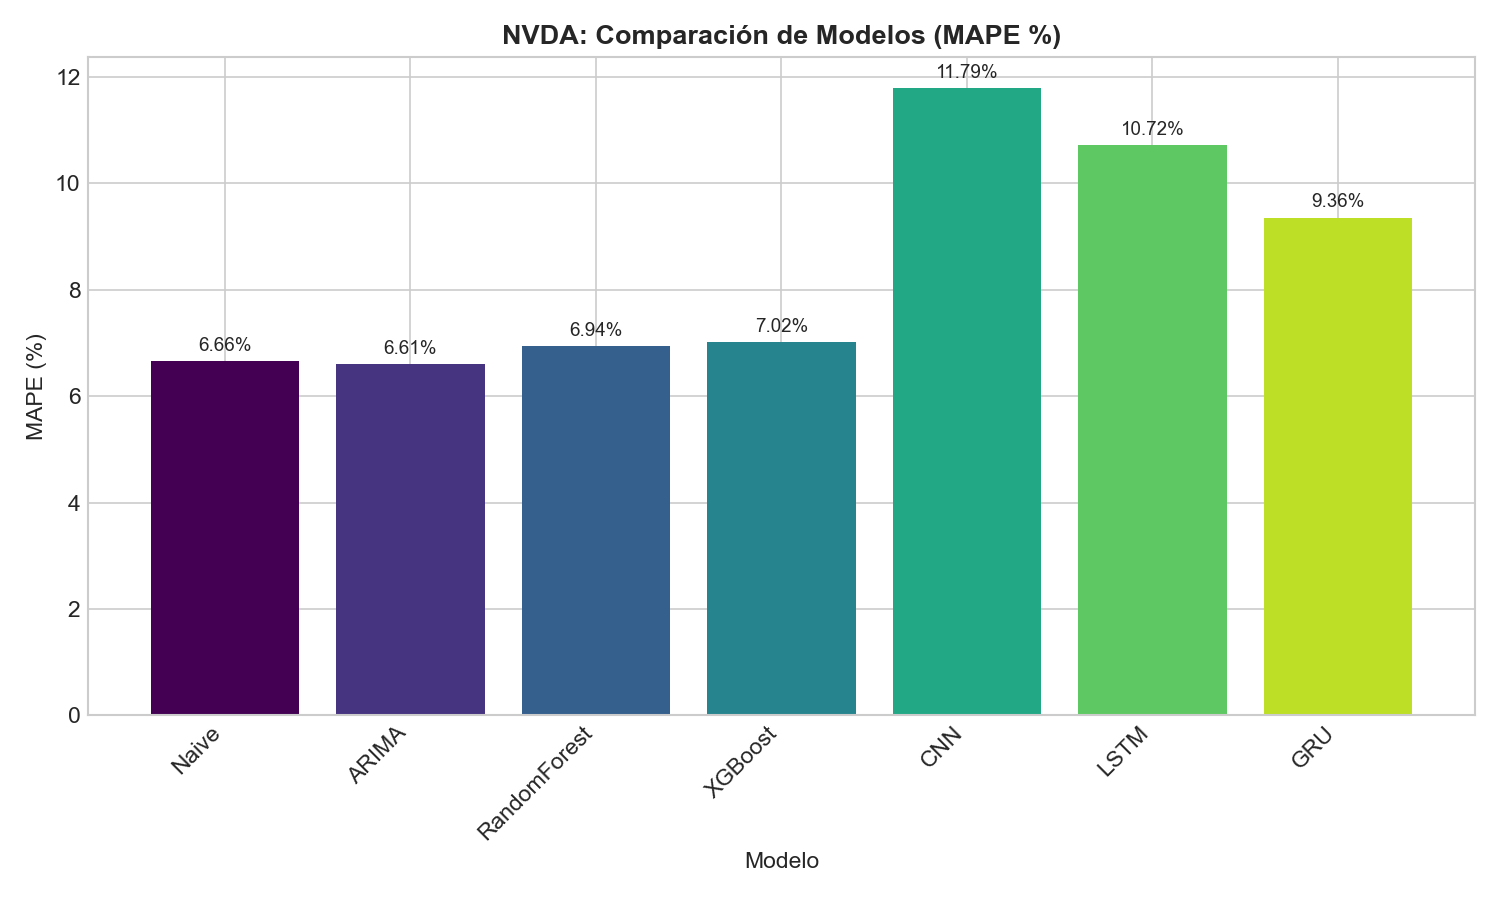
\includegraphics[width=0.95\textwidth]{Imagenes/model_comparison_NVDA_mape.png}
\caption{NVDA: Comparación de modelos (MAPE \%).}
\label{fig:model_nvda_mape}
\end{figure}

\begin{figure}[H]
\centering
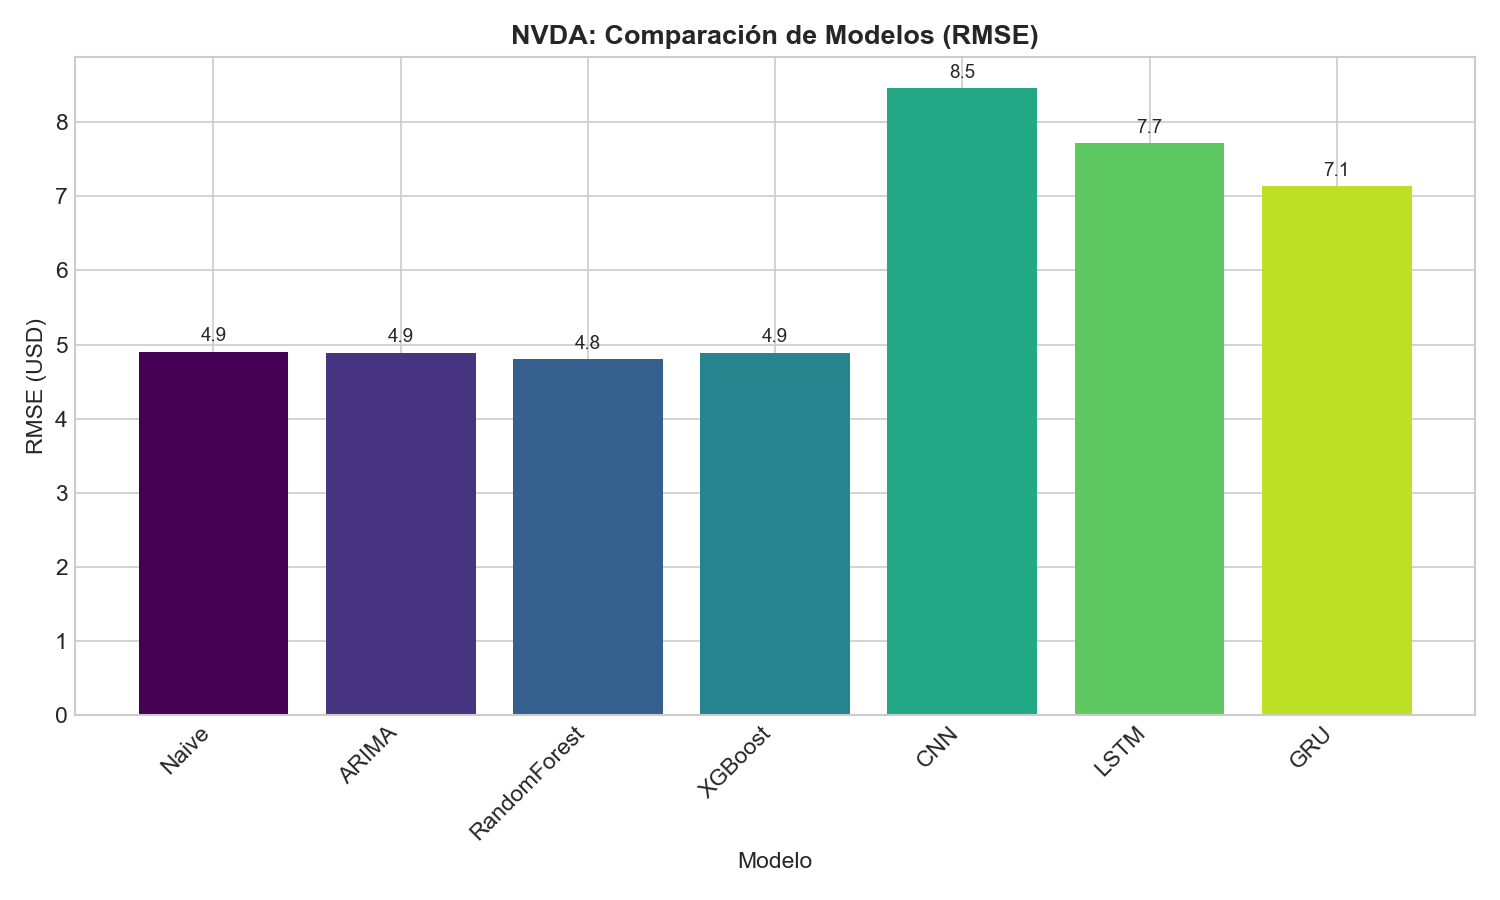
\includegraphics[width=0.95\textwidth]{Imagenes/model_comparison_NVDA_rmse.png}
\caption{NVDA: Comparación de modelos (RMSE en USD).}
\label{fig:model_nvda_rmse}
\end{figure}

En Nvidia, \textbf{ARIMA} marca el mejor MAPE, con Naive prácticamente empatado. Random Forest y XGBoost se quedan relativamente cerca pero no mejoran a los baselines. Las redes profundas vuelven a estar claramente por detrás (especialmente CNN y LSTM); GRU se aproxima más, pero no alcanza a ARIMA/Naive.

El hecho de que ARIMA y Naive estén tan próximos invita a no sobreinterpretar pequeñas diferencias: en un activo con cambios de régimen frecuentes, la estabilidad del rendimiento pesa casi tanto como la media.

\subsection{Visión de conjunto}

Para facilitar la comparación entre modelos y activos, se generaron varias visualizaciones de síntesis. La Figura~\ref{fig:cross_asset_heatmap} presenta un mapa de calor que resume el MAPE de cada modelo por activo. Los colores más fríos (azul) indican menor error y, por tanto, mejor rendimiento. Esta visualización permite identificar rápidamente qué combinaciones modelo-activo funcionan mejor y detectar patrones transversales.

\begin{figure}[H]
\centering
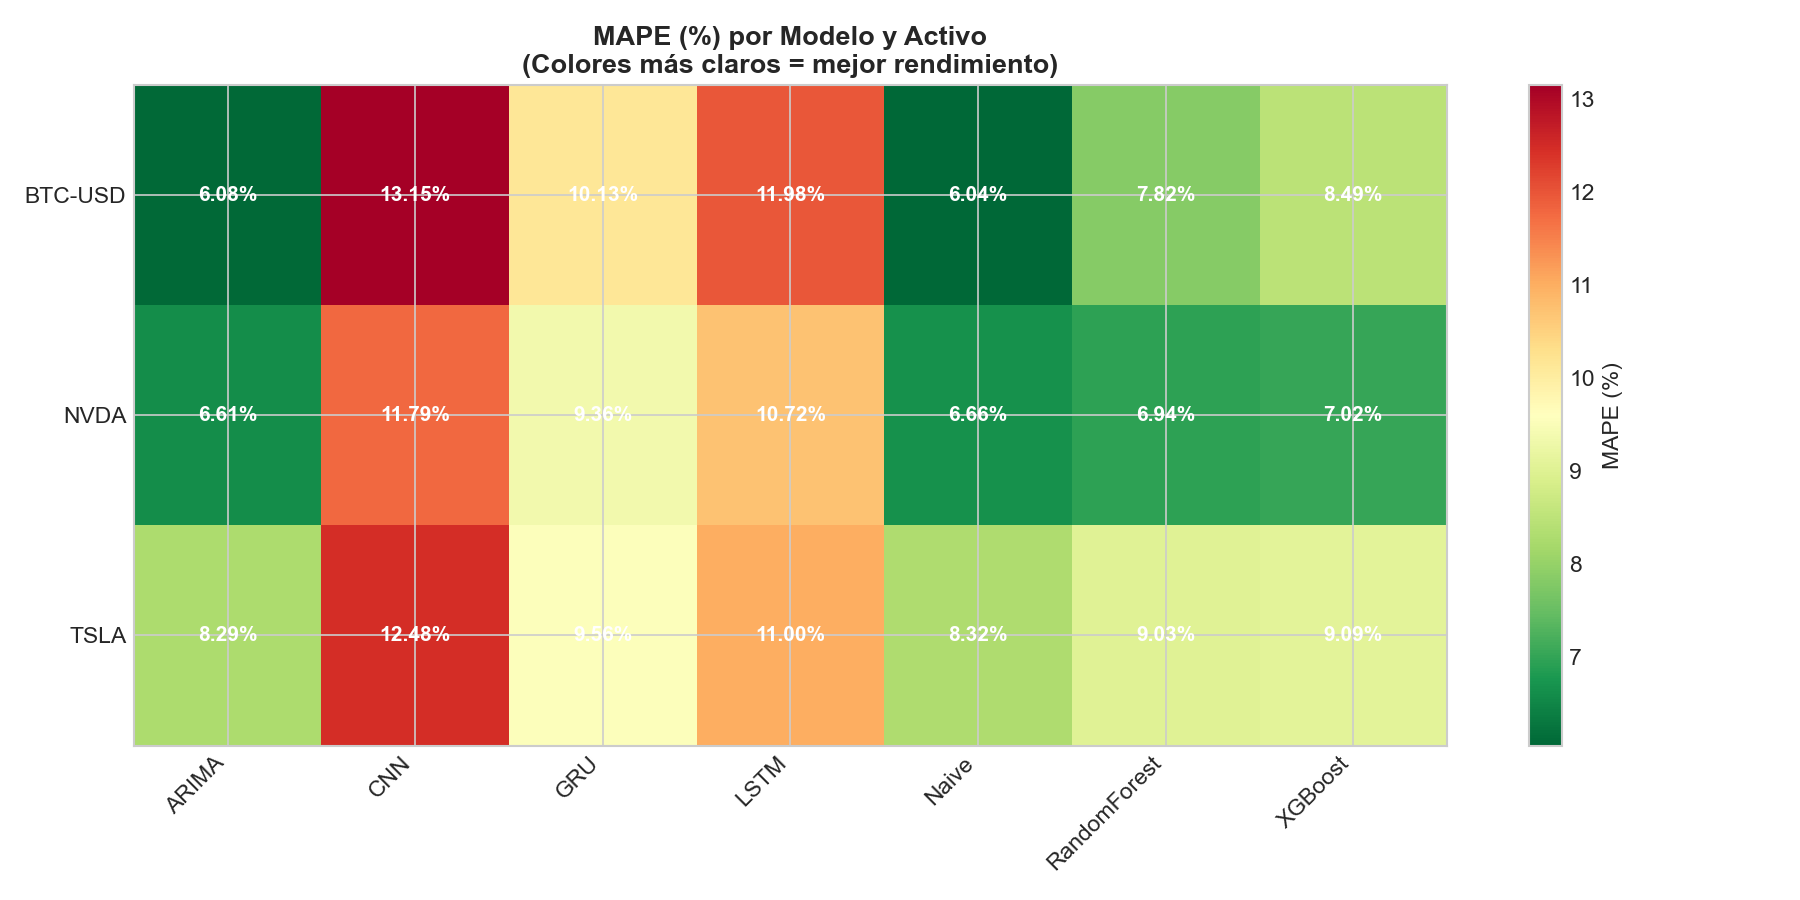
\includegraphics[width=0.95\textwidth]{Imagenes/cross_asset_heatmap.png}
\caption{Mapa de calor: MAPE (\%) por modelo y activo.}
\label{fig:cross_asset_heatmap}
\end{figure}

Complementando el mapa de calor, la Figura~\ref{fig:cross_asset_bar} presenta la misma información en formato de barras agrupadas, lo que facilita la comparación directa de la magnitud del error entre modelos dentro de cada activo. Este formato es especialmente útil para identificar cuánto mejor o peor es cada modelo respecto a los demás en términos absolutos.

\begin{figure}[H]
\centering
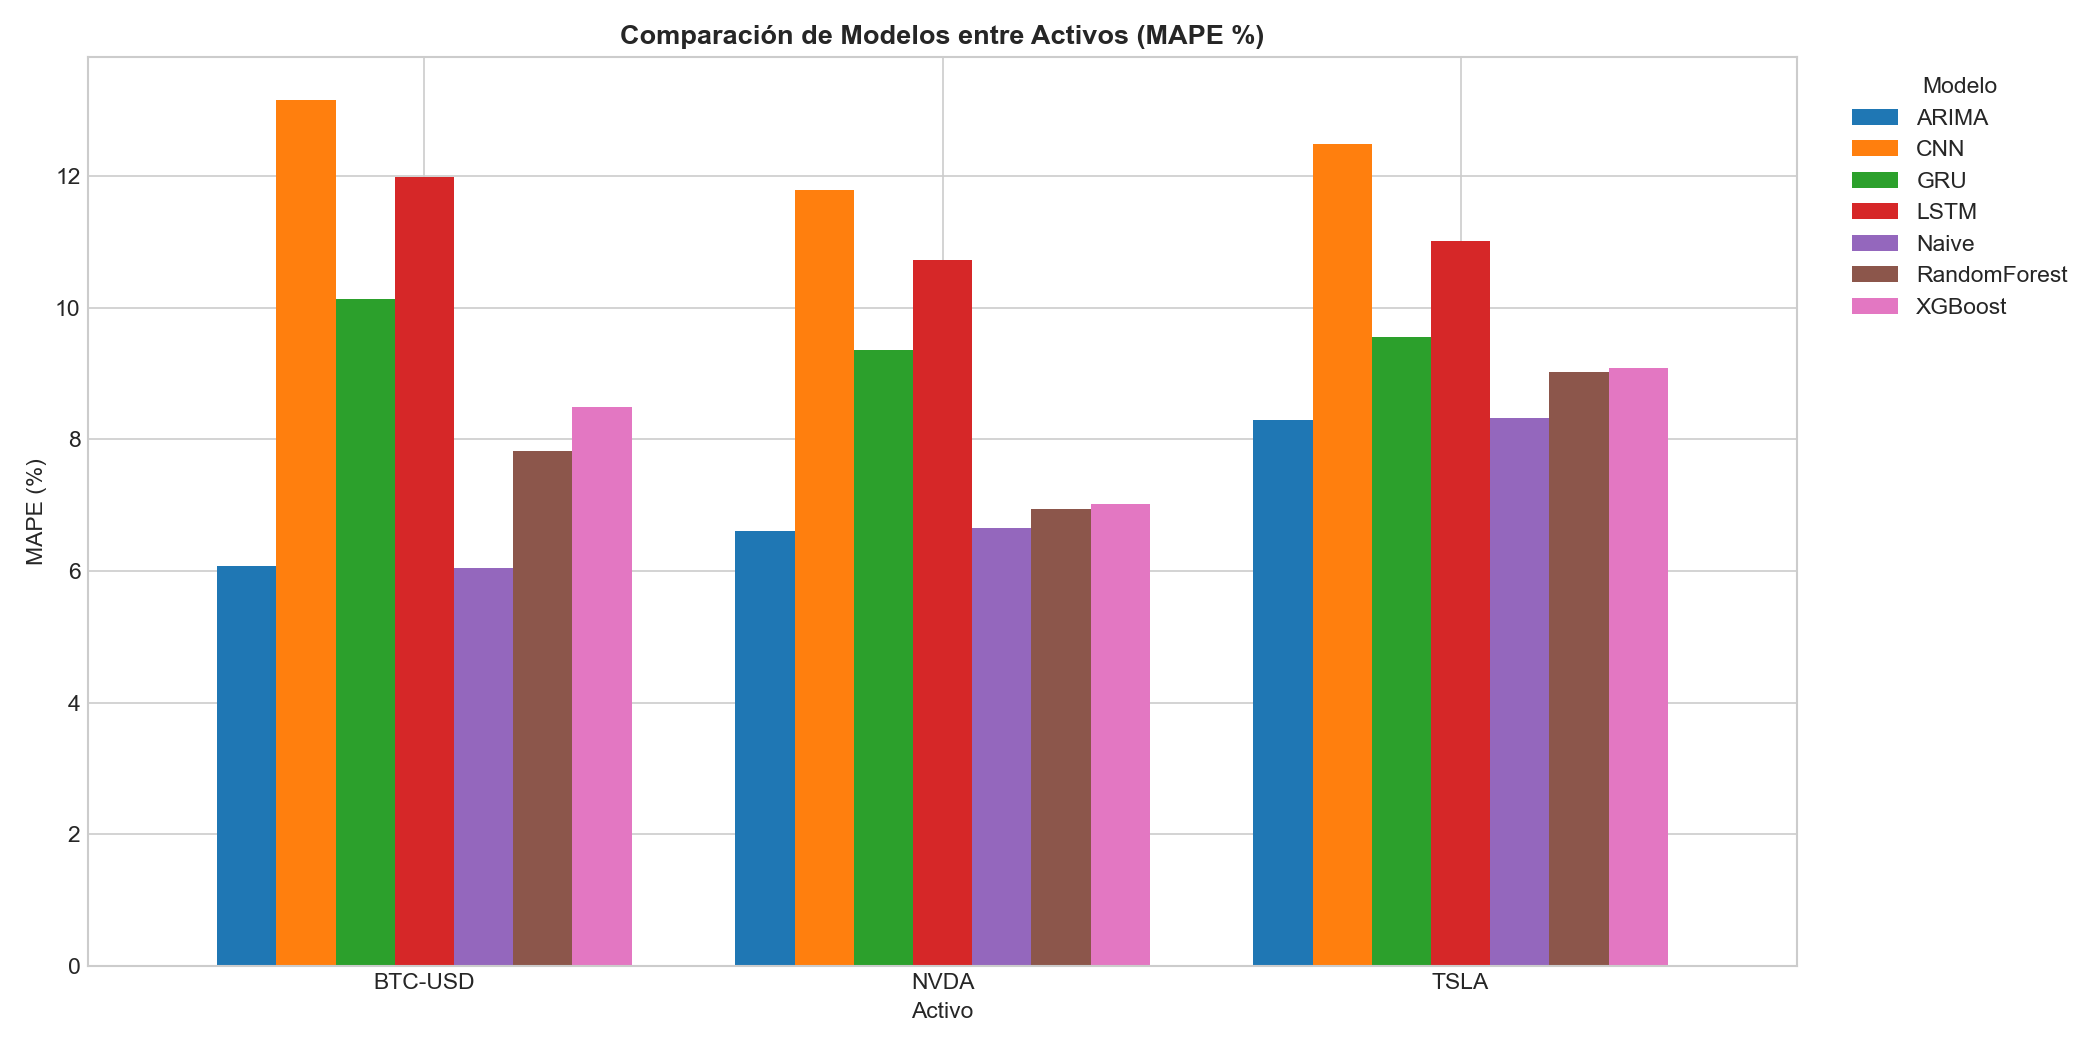
\includegraphics[width=0.95\textwidth]{Imagenes/cross_asset_grouped_bar.png}
\caption{Comparación agrupada de modelos entre activos.}
\label{fig:cross_asset_bar}
\end{figure}

Además de comparar medias, resulta fundamental analizar la dispersión del error. La Figura~\ref{fig:error_dist_all} muestra la distribución del MAPE mediante diagramas de caja (boxplots). Esta visualización permite identificar no solo qué modelo tiene menor error medio, sino también cuál presenta mayor estabilidad en sus predicciones. Un modelo con baja mediana pero alta dispersión (caja ancha) puede ser menos fiable en la práctica que otro con error algo mayor pero más consistente.

\begin{figure}[H]
\centering
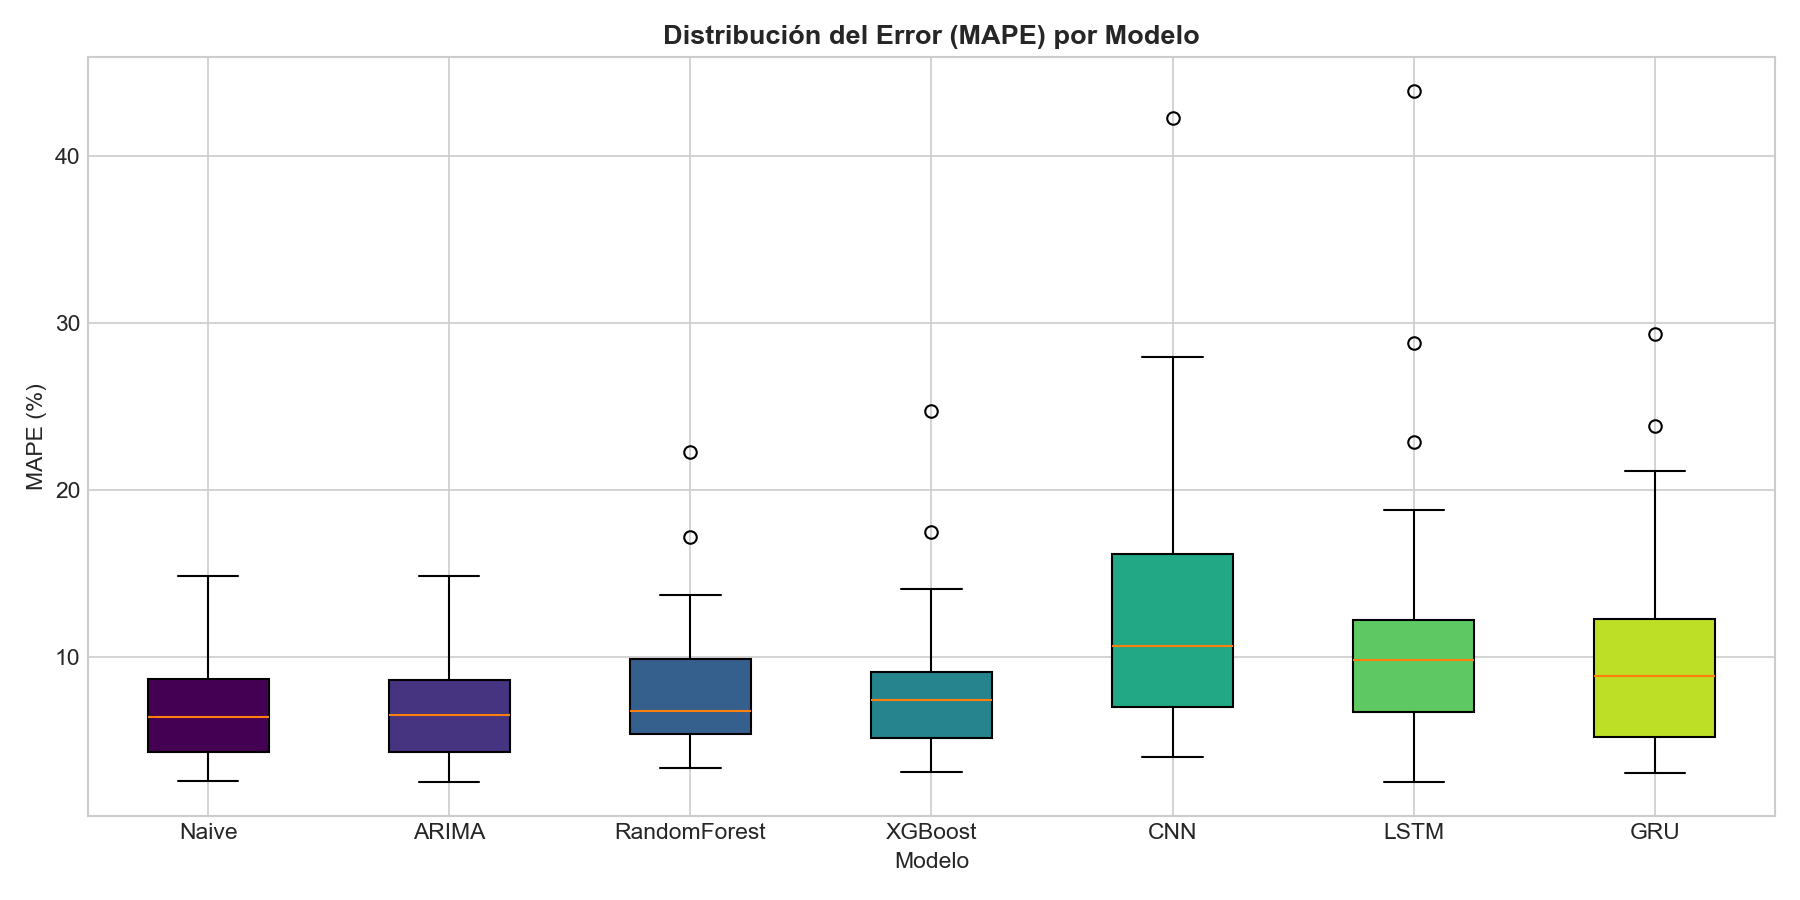
\includegraphics[width=0.95\textwidth]{Imagenes/error_distribution_boxplot.png}
\caption{Distribución del error MAPE por modelo.}
\label{fig:error_dist_all}
\end{figure}

Además de la media, resulta útil ver la dispersión por fold. La Figura~\ref{fig:mape_dispersion} resume el MAPE medio y su variabilidad, que ayuda a distinguir modelos estables de modelos con rendimiento errático.

\begin{figure}[H]
\centering
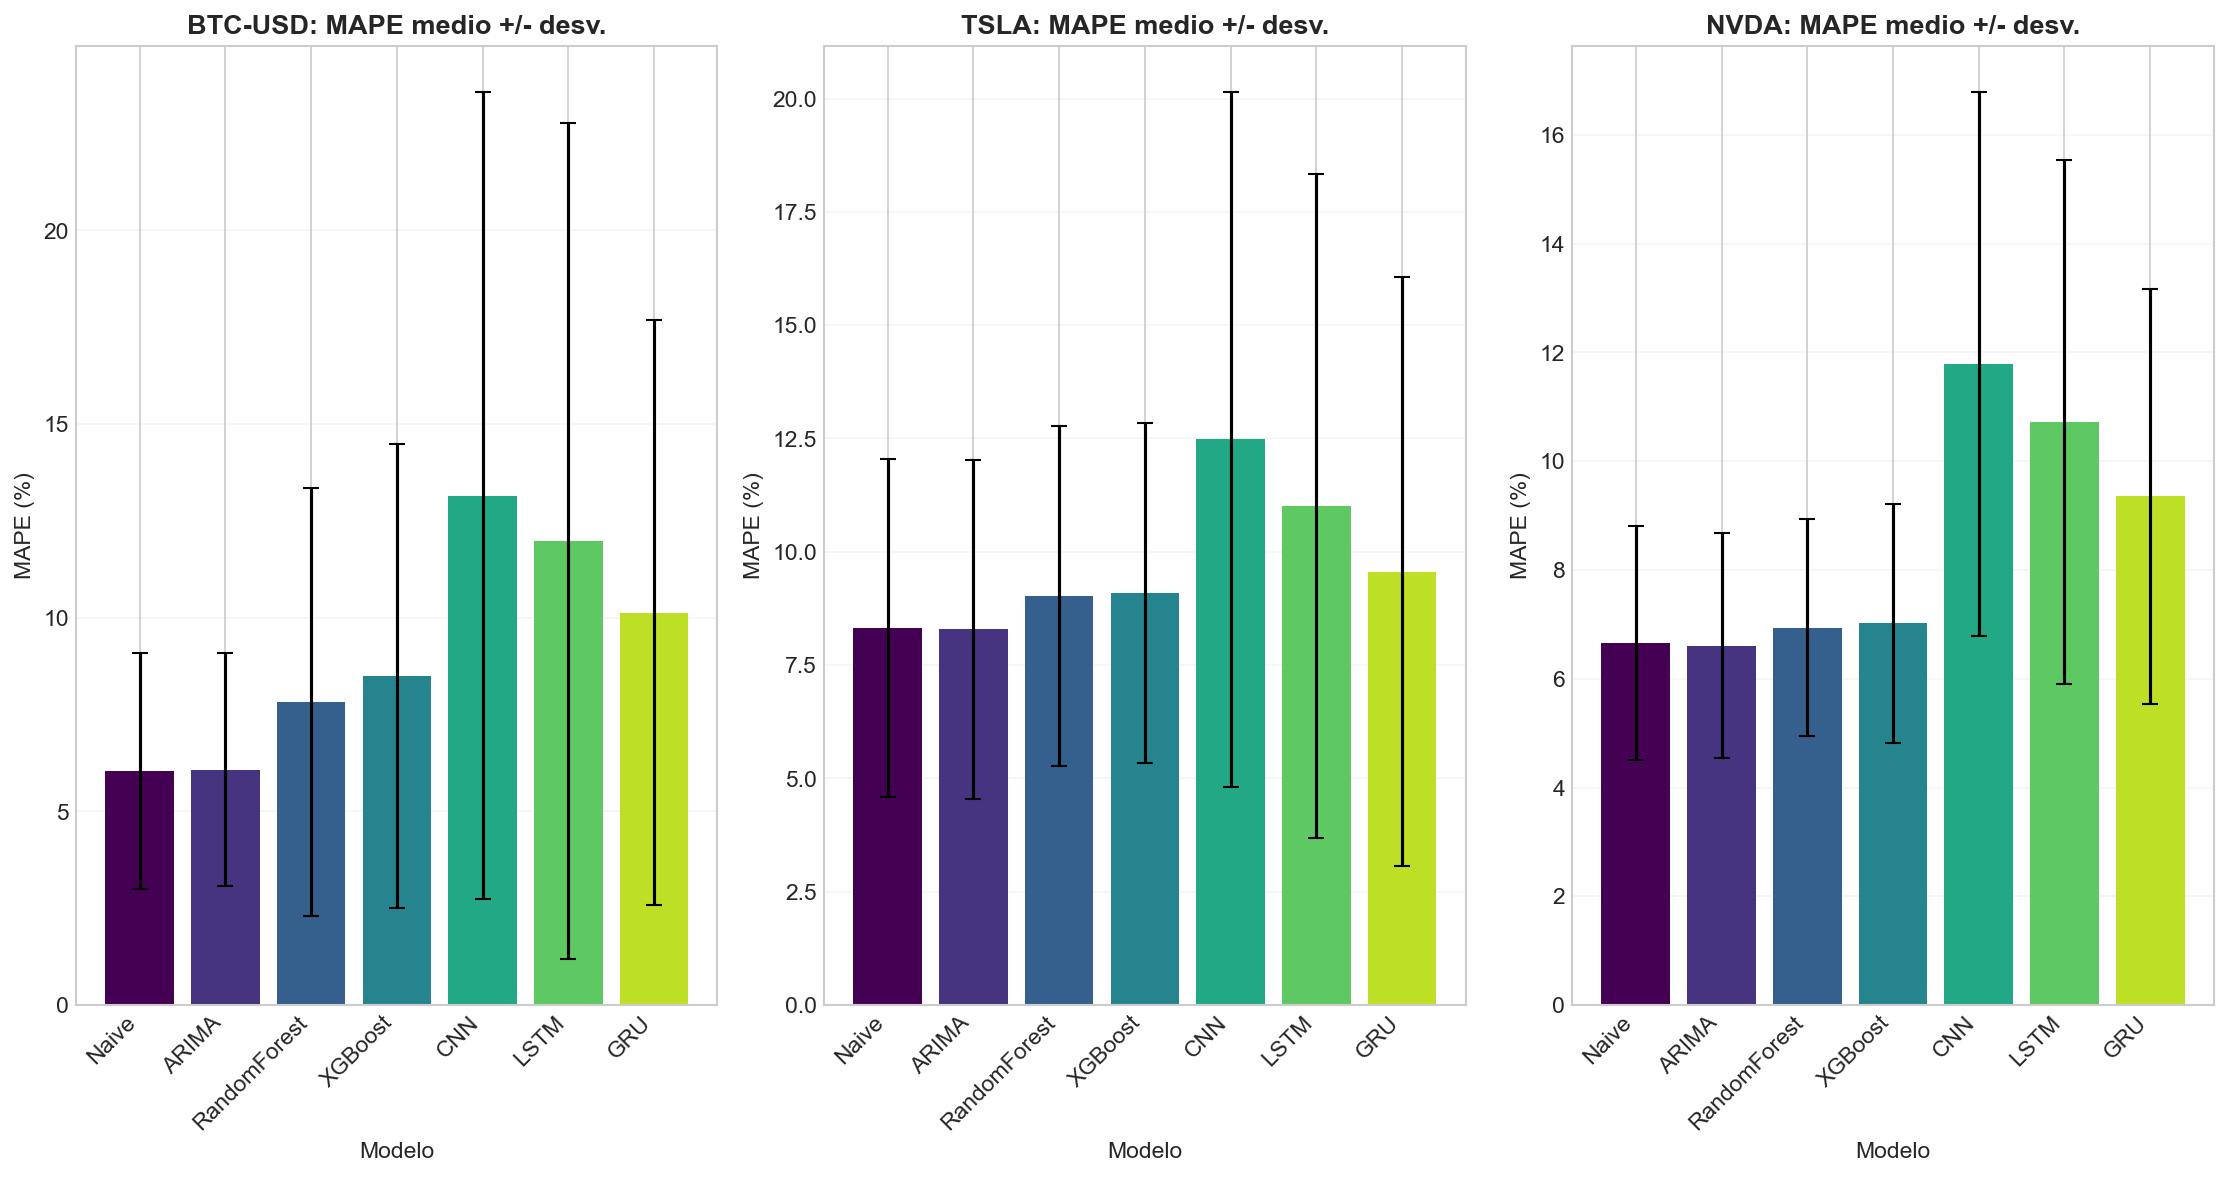
\includegraphics[width=0.95\textwidth]{Imagenes/model_comparison_mape_dispersion.png}
\caption{MAPE medio y dispersión por fold en cada activo.}
\label{fig:mape_dispersion}
\end{figure}

Estas tres vistas (heatmap, barras y boxplot) reflejan el mismo patrón desde perspectivas distintas: los baselines lideran de forma consistente y la dispersión de errores es relevante al comparar modelos no-baseline. En la práctica, un modelo con mejor media pero muy inestable puede ser peor elección que otro ligeramente peor pero más consistente.

Implicación práctica: si se necesita un modelo ``por defecto'' para repetir este experimento, \textbf{ARIMA} y \textbf{Naive} son referencias muy fuertes (Naive lidera BTC-USD y ARIMA lidera TSLA/NVDA). En este trabajo, ni los modelos de árboles ni los modelos DL justifican su complejidad frente a esos baselines en términos de MAPE.

%% ============================================================
%% EXPERIMENTO B: IMPACTO DEL HORIZONTE
%% ============================================================

\section{Impacto del horizonte de predicción (BTC-USD)}

Era previsible que la predicción resultara más difícil a mayor horizonte. La incertidumbre se acumula y la probabilidad de que ocurra algo inesperado crece con los días. Este experimento cuantifica dicha expectativa.

\subsection{Los números}

La Tabla~\ref{tab:experiment_b} compara los horizontes de 1, 7 y 30 días para Bitcoin.

\begin{table}[H]
\centering
\caption{MAPE (\%) por horizonte para BTC-USD}
\label{tab:experiment_b}
\begin{tabular}{l|ccc}
\hline
\textbf{Modelo} & \textbf{1 dia} & \textbf{7 dias} & \textbf{30 dias} \\
\hline
CNN & 7.71 & 13.15 & 20.93 \\
GRU & \textbf{5.58} & \textbf{10.13} & \textbf{20.11} \\
LSTM & 8.11 & 11.98 & 26.16 \\
\hline
\end{tabular}
\end{table}

Como era de esperar, todos los modelos empeoran a medida que aumenta el horizonte. En BTC-USD el salto es sustancial: el MAPE pasa de un orden del 5--8\% a 1 día a valores cercanos al 20\% a 30 días. Dentro de los modelos DL, GRU es el más consistente y mantiene el menor MAPE en los tres horizontes; LSTM y CNN degradan más, especialmente a 30 días. La Figura~\ref{fig:horizon_all_models} ilustra esta degradación.

\begin{figure}[H]
\centering
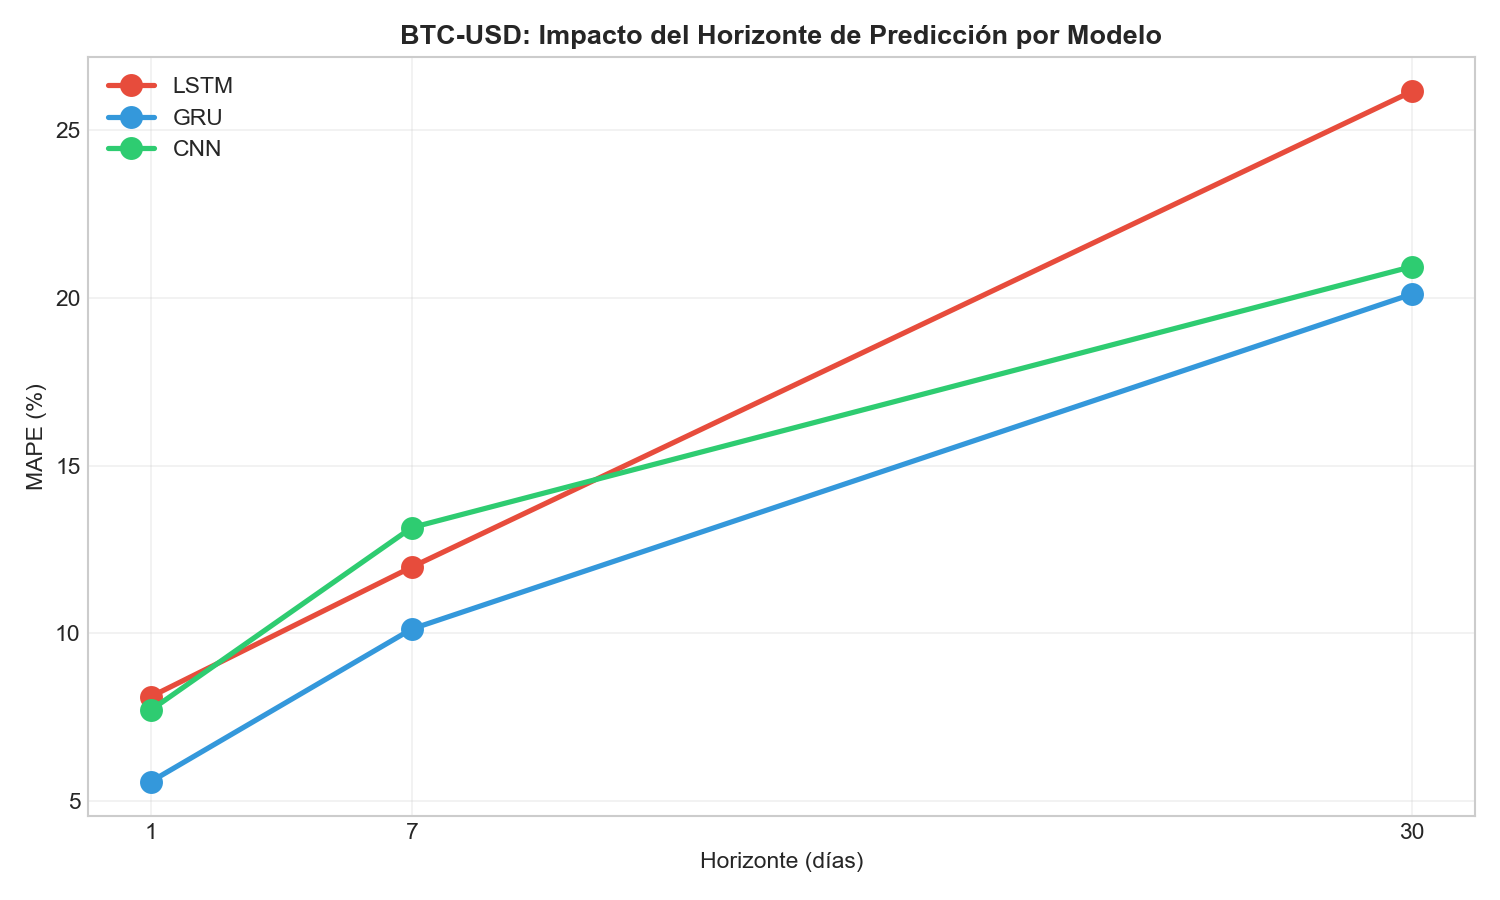
\includegraphics[width=0.90\textwidth]{Imagenes/horizon_impact_all_models.png}
\caption{Impacto del horizonte por modelo.}
\label{fig:horizon_all_models}
\end{figure}

Para analizar en detalle cómo se comporta cada arquitectura a medida que aumenta el horizonte, las Figuras~\ref{fig:horizon_lstm}, \ref{fig:horizon_gru} y \ref{fig:horizon_cnn} desglosan las métricas (RMSE, MAE y MAPE) por modelo. Estas visualizaciones permiten identificar no solo cuál modelo escala mejor, sino también detectar comportamientos anómalos ---por ejemplo, que un modelo degrade más rápido de lo esperado o que mantenga su rendimiento de forma atípica---.

\begin{figure}[H]
\centering
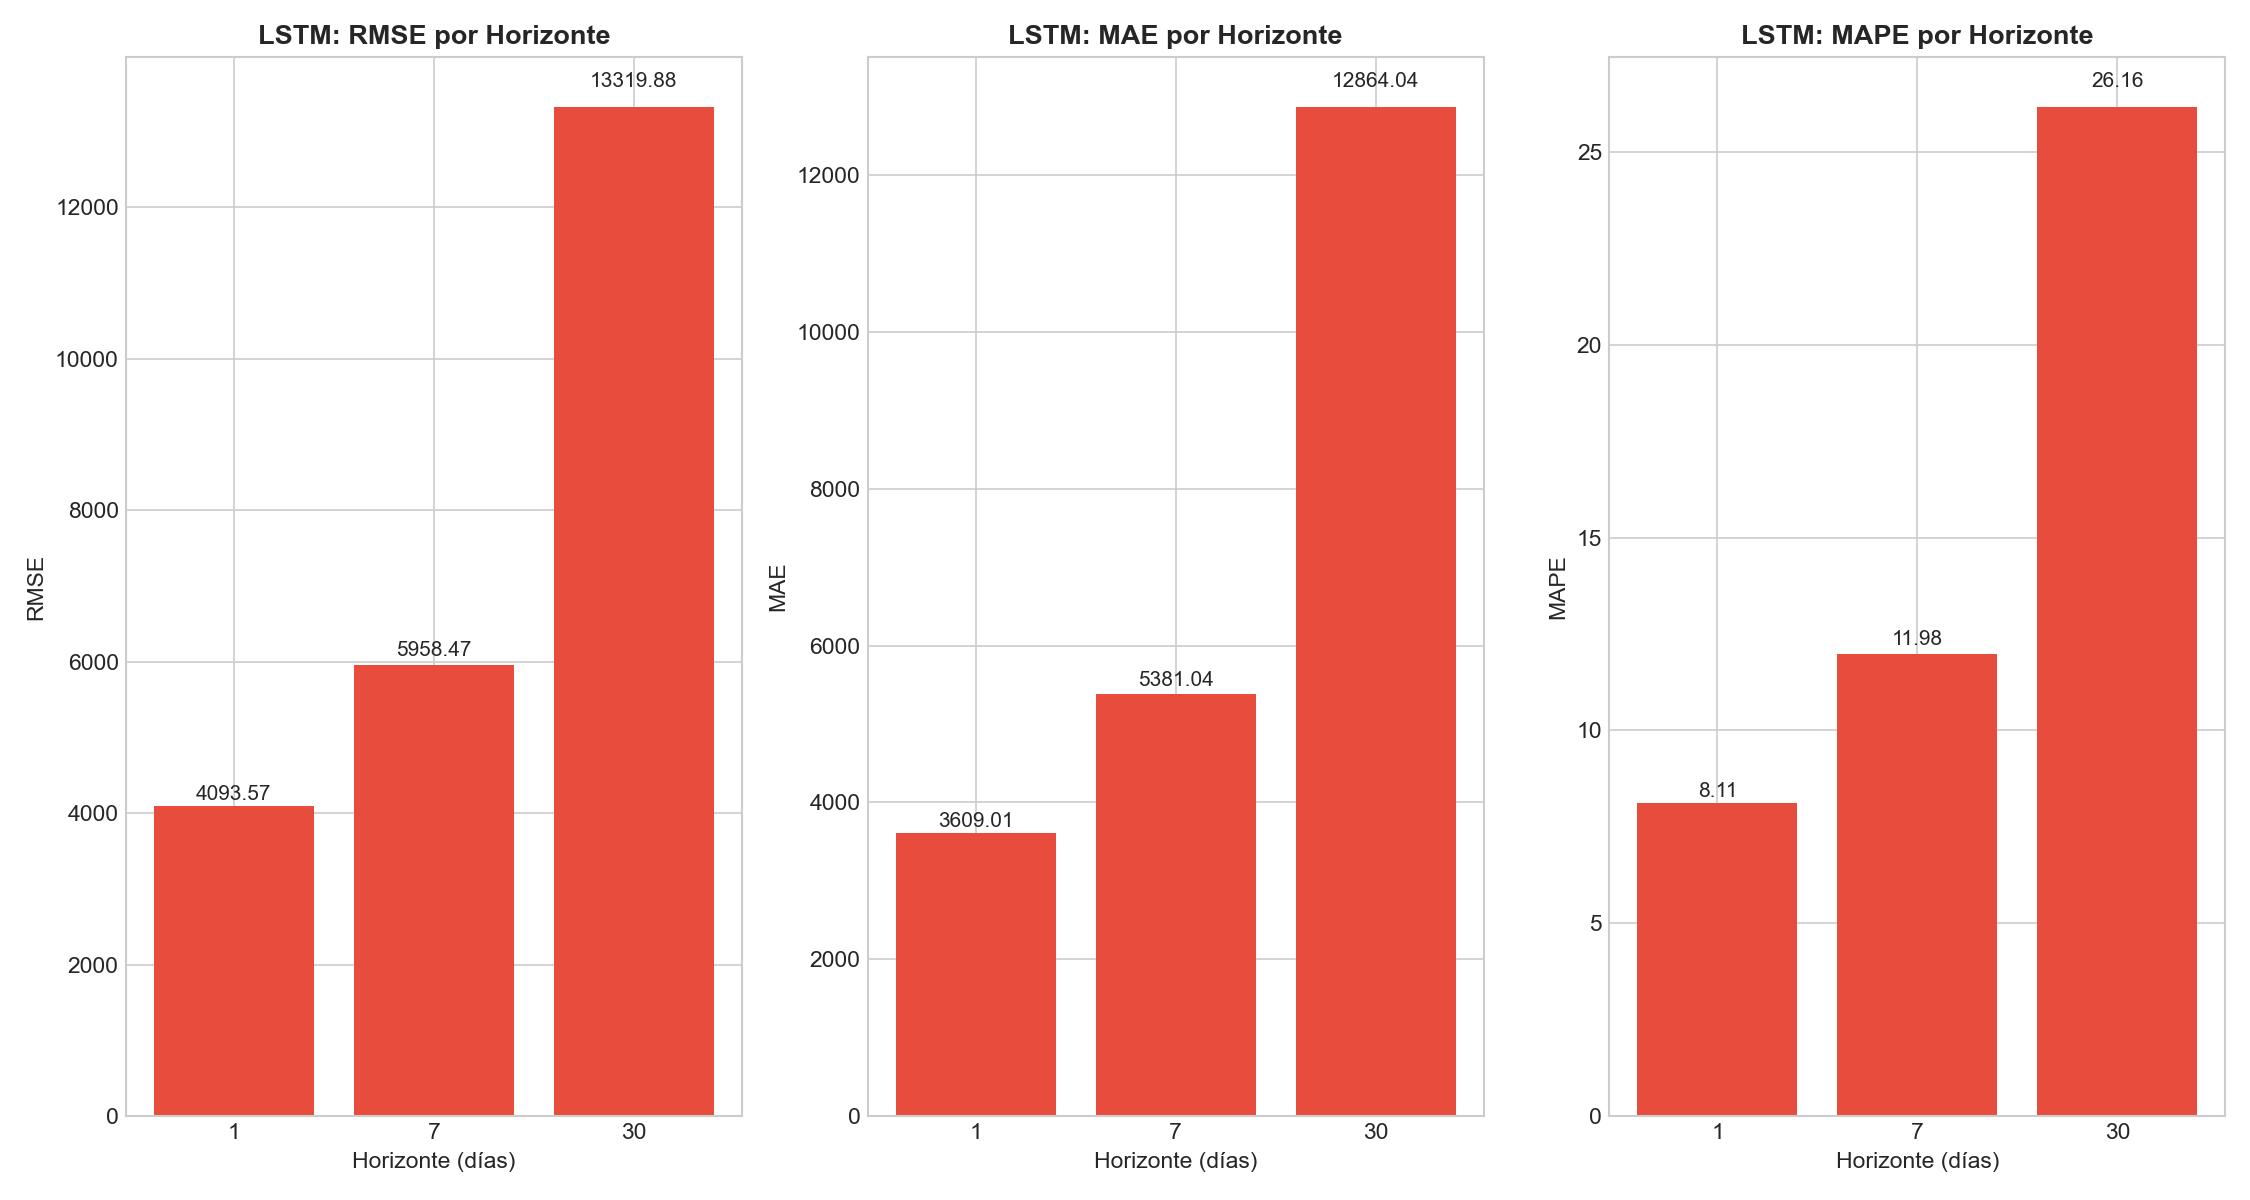
\includegraphics[width=0.95\textwidth]{Imagenes/horizon_impact_lstm_metrics.png}
\caption{LSTM: Métricas por horizonte. El error aumenta de forma marcada a medida que se alarga el horizonte, especialmente a 30 días.}
\label{fig:horizon_lstm}
\end{figure}

\begin{figure}[H]
\centering
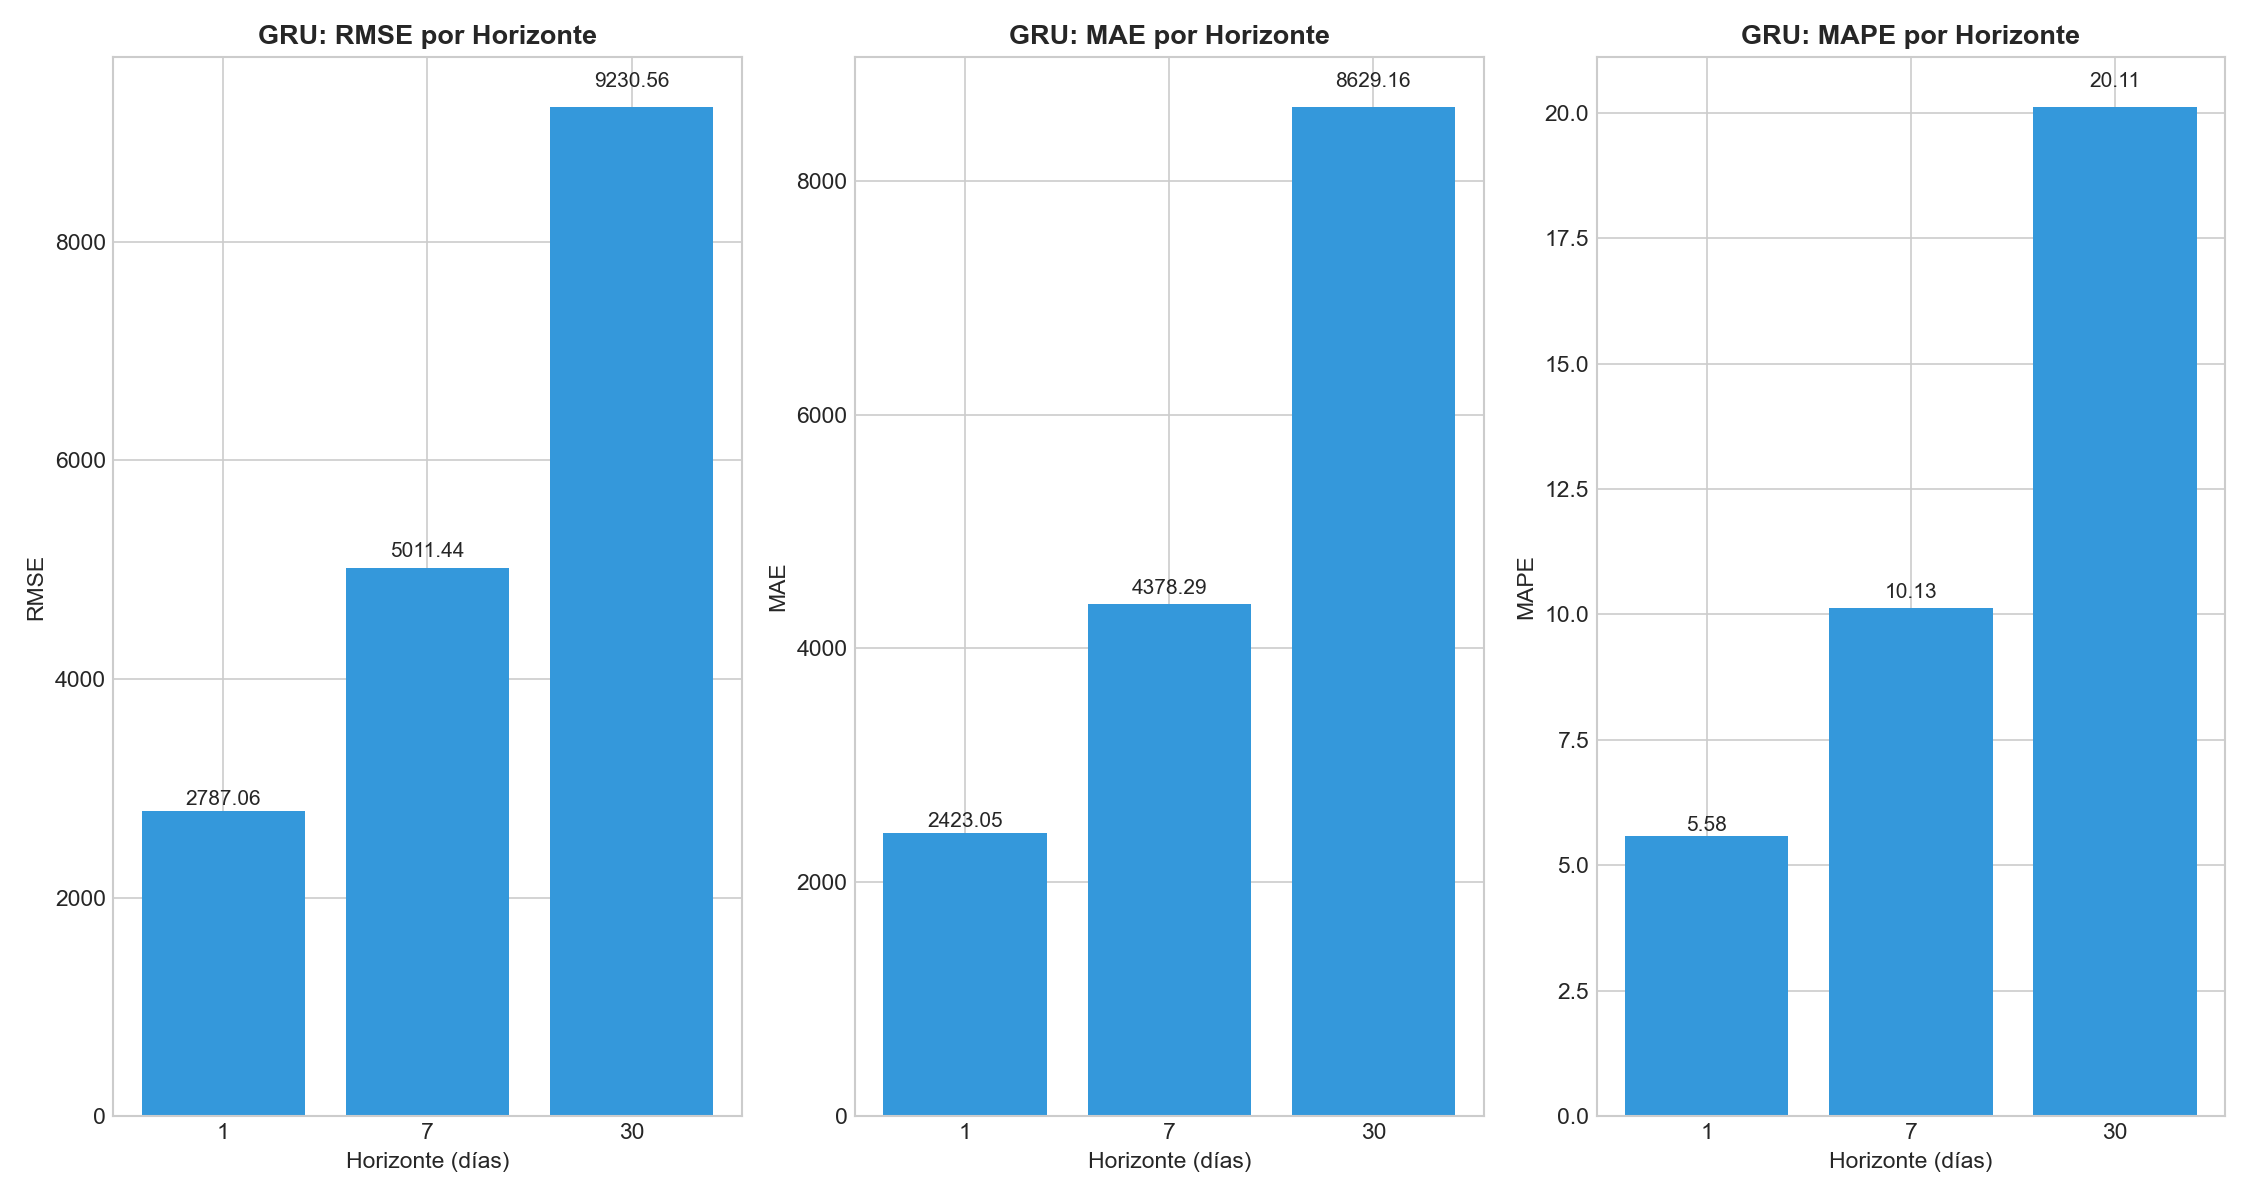
\includegraphics[width=0.95\textwidth]{Imagenes/horizon_impact_gru_metrics.png}
\caption{GRU: Métricas por horizonte. GRU muestra el comportamiento más estable de las tres arquitecturas, con una degradación más suave y valores consistentemente inferiores a LSTM y CNN en todos los horizontes.}
\label{fig:horizon_gru}
\end{figure}

\begin{figure}[H]
\centering
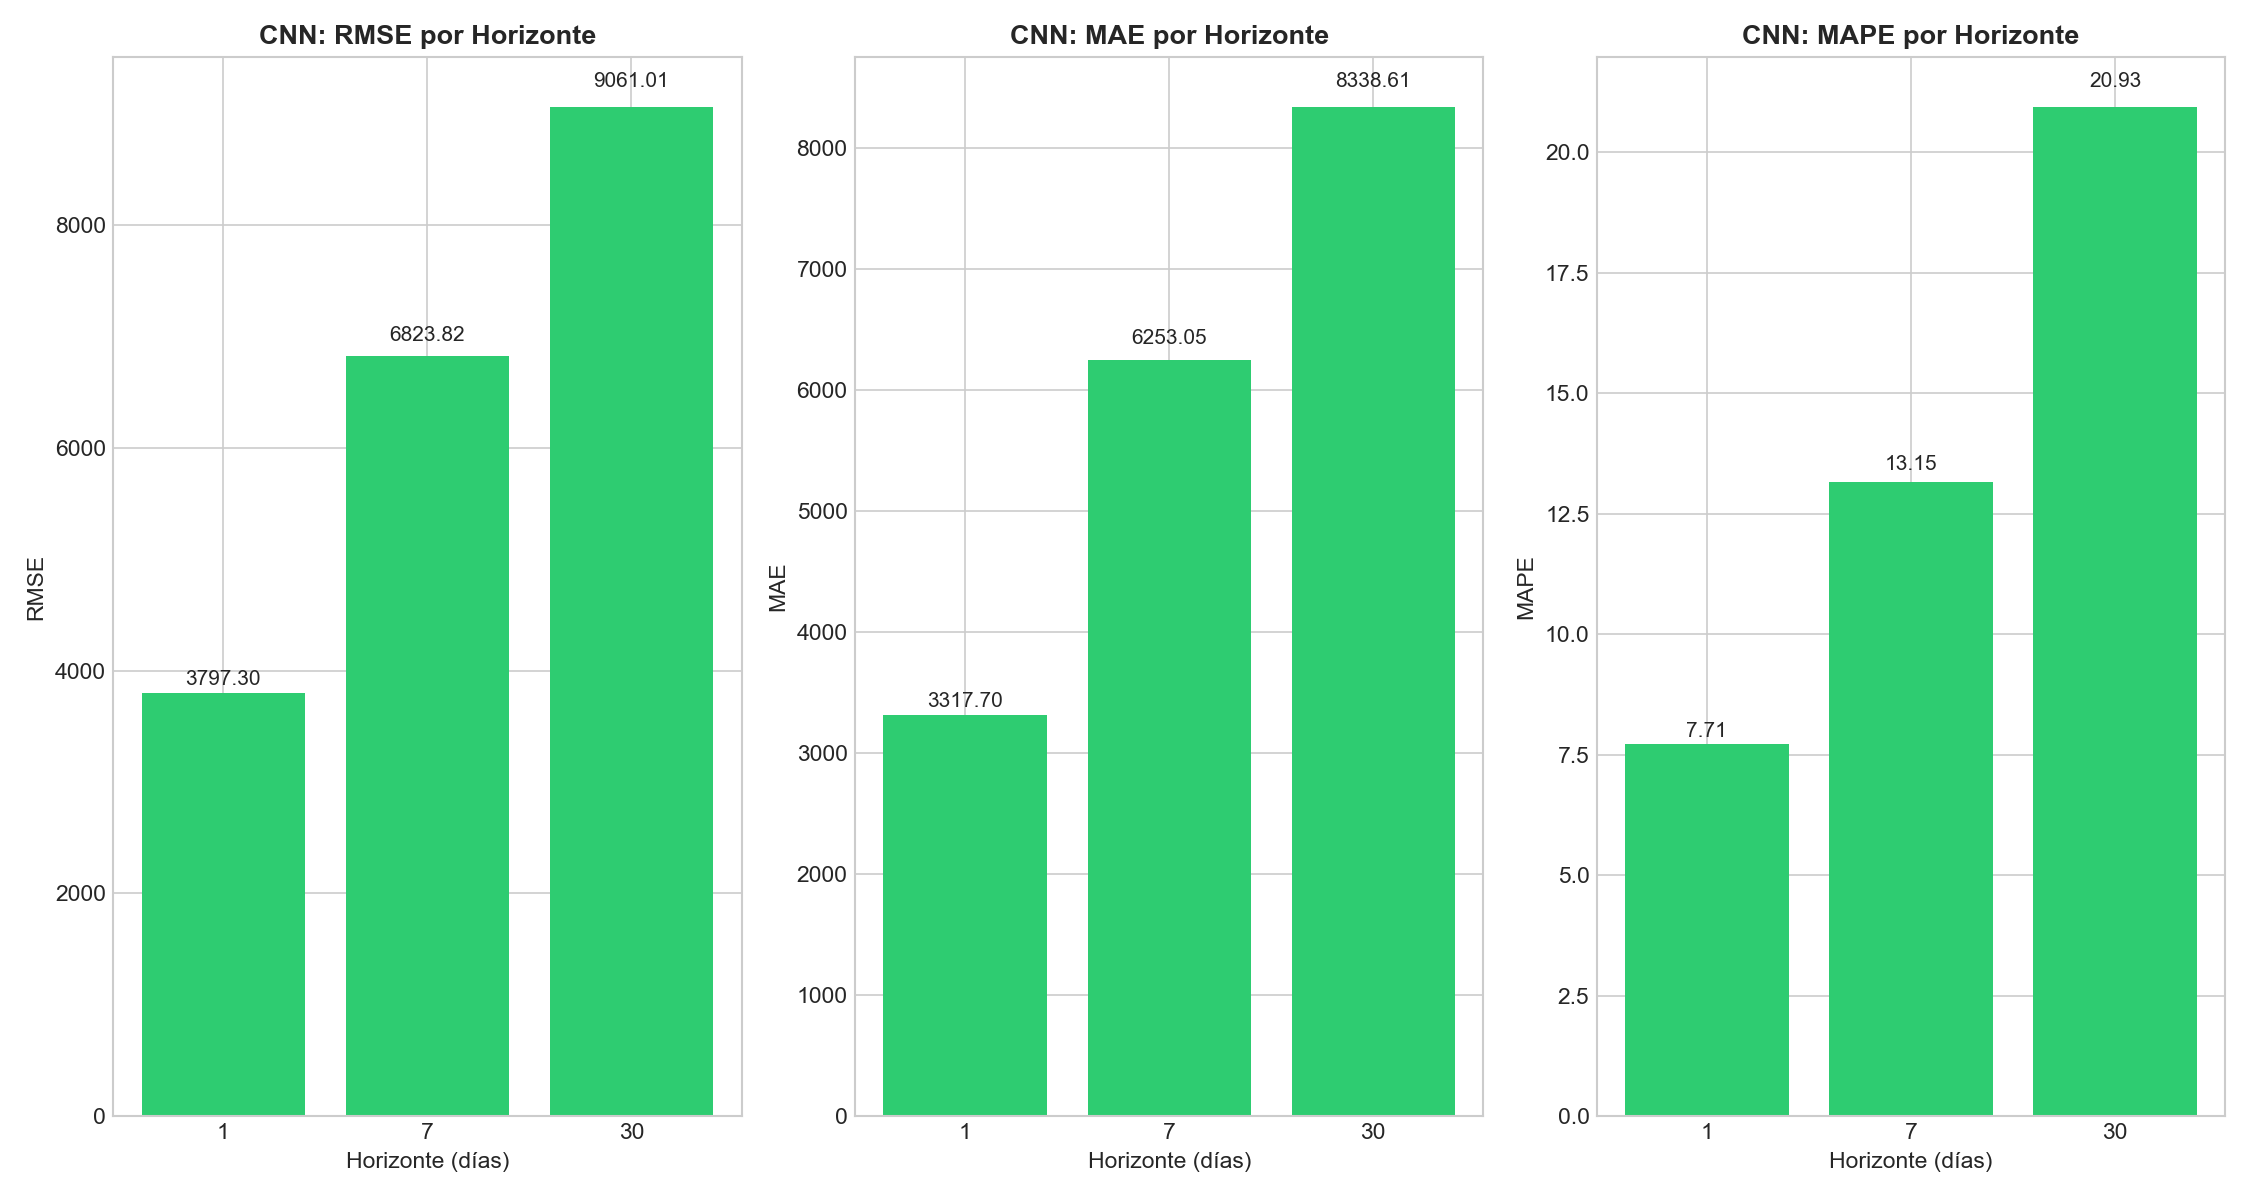
\includegraphics[width=0.95\textwidth]{Imagenes/horizon_impact_cnn_metrics.png}
\caption{CNN: Métricas por horizonte. CNN es la arquitectura que peor escala con el horizonte: aunque a 1 día se mueve en rangos similares, a 30 días el error aumenta de forma más pronunciada, evidenciando su limitación para capturar dependencias de largo plazo.}
\label{fig:horizon_cnn}
\end{figure}

La lección es clara dentro de la familia DL: GRU es el más robusto en todos los horizontes, aunque a 30 días los errores ya son altos. CNN, por el contrario, es la arquitectura que más sufre cuando el horizonte se alarga, lo que sugiere que su mecanismo de convolución local no captura adecuadamente las dependencias temporales extendidas necesarias para predicciones a largo plazo.

Desde un punto de vista operativo, esto pone un límite práctico: cuanto más lejos se intenta predecir, mayor es el coste en error. Si el objetivo es apoyar decisiones a corto plazo, el horizonte de 7 días parece un compromiso razonable; para 30 días, la señal se diluye demasiado.

Implicación práctica: si la predicción va a usarse en un contexto real, resulta más conveniente optimizar horizontes cortos y consistentes que perseguir horizontes largos con errores elevados.

%% ============================================================
%% EXPERIMENTO C: ABLACIÓN DE SENTIMIENTO
%% ============================================================

\section{Ablación de sentimiento (con vs sin)}

Este es el experimento central del trabajo. Se ejecutaron los modelos con y sin sentimiento para comprobar si contribuye de forma significativa a la predicción. El resultado principal es que el efecto existe, pero es \textbf{pequeño, y depende mucho del activo y del modelo}.

\subsection{Los números clave}

La Tabla~\ref{tab:experiment_c_full} muestra los resultados completos para todos los modelos de deep learning.

\begin{table}[H]
\centering
\caption{MAPE (\%) por modelo y activo, con y sin sentimiento}
\label{tab:experiment_c_full}
\begin{tabular}{l|l|cc|c}
\hline
\textbf{Activo} & \textbf{Modelo} & \textbf{Con Sent.} & \textbf{Sin Sent.} & \textbf{Ayuda?} \\
\hline
BTC-USD & CNN & 13.15 & 10.51 & \textcolor{red}{No (-25.1\%)} \\
BTC-USD & GRU & 10.13 & 9.16 & \textcolor{red}{No (-10.6\%)} \\
BTC-USD & LSTM & 11.98 & 10.94 & \textcolor{red}{No (-9.5\%)} \\
NVDA & CNN & 11.79 & 10.71 & \textcolor{red}{No (-10.1\%)} \\
NVDA & GRU & 9.36 & 8.95 & \textcolor{red}{No (-4.6\%)} \\
NVDA & LSTM & 10.72 & 10.96 & \textcolor{green!60!black}{Si (2.2\%)} \\
TSLA & CNN & 12.48 & 12.95 & \textcolor{green!60!black}{Si (3.6\%)} \\
TSLA & GRU & 9.56 & 9.82 & \textcolor{green!60!black}{Si (2.7\%)} \\
TSLA & LSTM & 11.00 & 11.32 & \textcolor{green!60!black}{Si (2.8\%)} \\
\hline
\end{tabular}
\end{table}

Los resultados muestran un patrón heterogéneo. El sentimiento \textbf{puede ayudar o perjudicar} según el activo:

\textbf{En Bitcoin, el sentimiento perjudica en los tres modelos.} El deterioro es especialmente marcado en CNN.

\textbf{En Tesla, el sentimiento mejora en los tres modelos.} La mejora existe, pero es moderada (del orden de unos pocos puntos porcentuales).

\textbf{En Nvidia, el efecto es mixto.} LSTM mejora ligeramente, mientras que CNN y GRU empeoran.

Estas diferencias pueden interpretarse como consecuencia de la naturaleza agregada de la señal de sentimiento y de la forma en que cada arquitectura integra variables externas. Bajo este protocolo, no se observa un patrón universal.

Estos resultados deben leerse en clave relativa. El test total es de 360 días, lo que mejora la estabilidad, pero un cambio de periodo puede mover bastante los porcentajes. Son resultados indicativos, no concluyentes; se discute de nuevo en la sección de limitaciones del capítulo final. La columna con sentimiento coincide con el experimento A; la comparación relevante es el salto frente a la columna sin sentimiento en cada modelo.

El porcentaje de mejora se calcula como $(\text{MAPE}_{\text{sin}} - \text{MAPE}_{\text{con}}) / \text{MAPE}_{\text{sin}}$. Valores positivos implican reducción del error al incluir sentimiento; valores negativos, empeoramiento. Las Figuras~\ref{fig:ablation_btc}--\ref{fig:ablation_nvda} muestran la ablación por activo, y la Figura~\ref{fig:ablation_heatmap} sintetiza los porcentajes de mejora en un mapa de calor.

\begin{figure}[H]
\centering
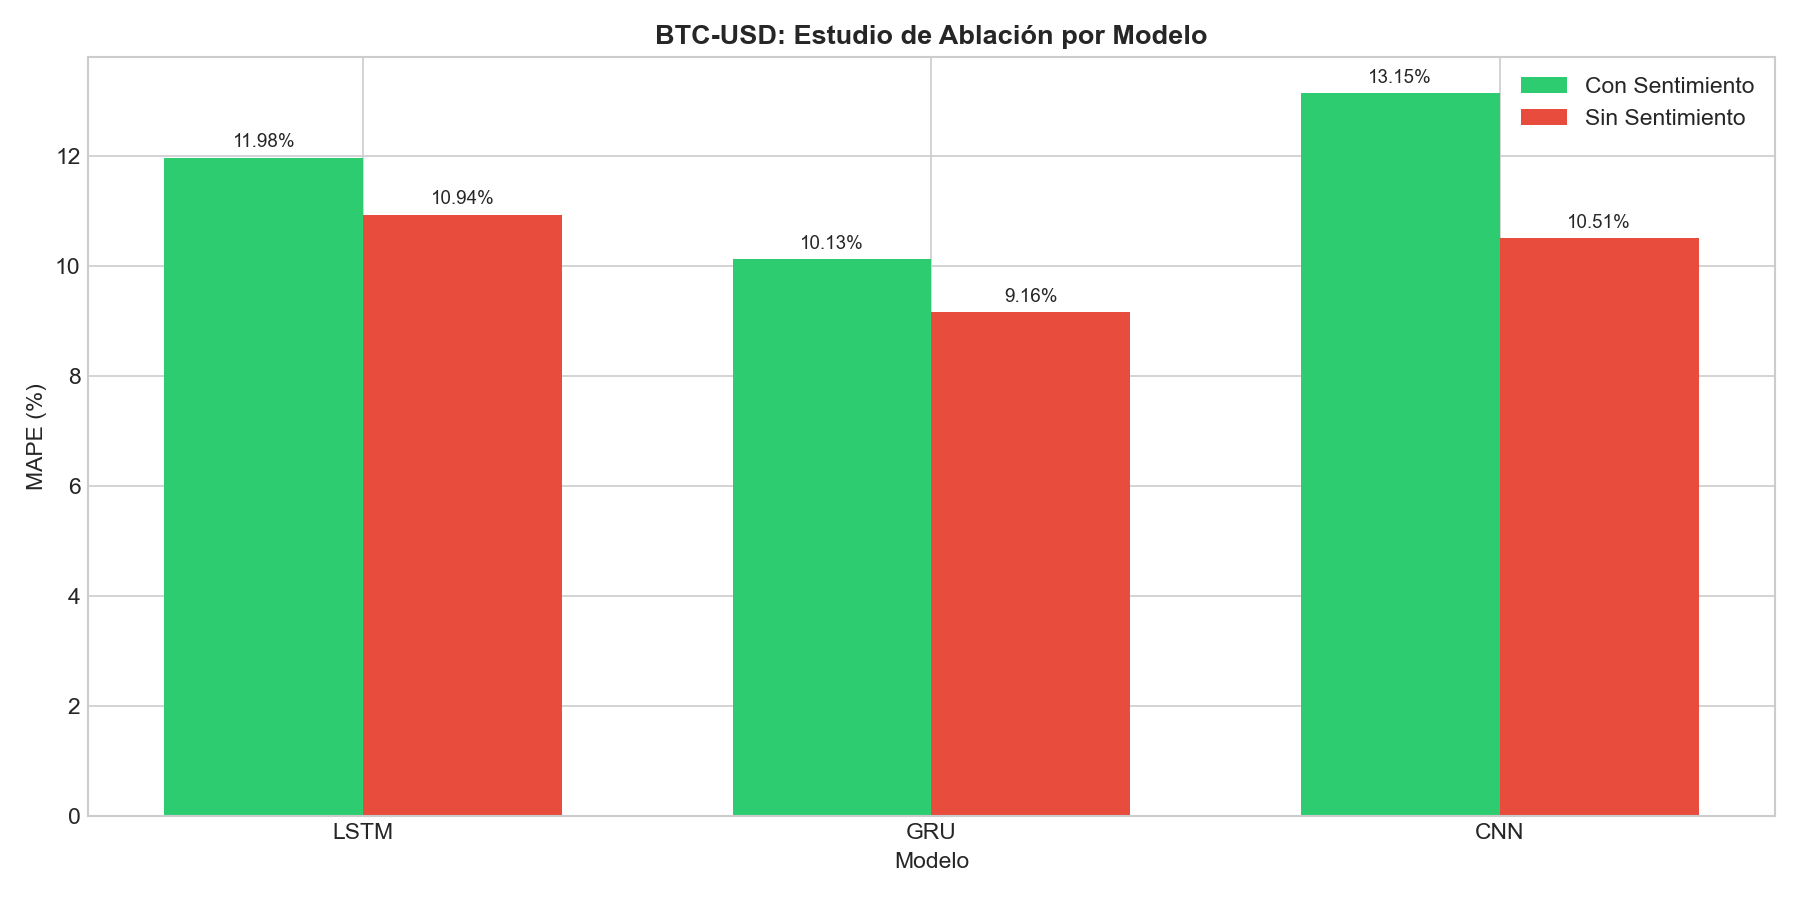
\includegraphics[width=0.90\textwidth]{Imagenes/ablation_BTC_USD_all_models.png}
\caption{BTC-USD: Ablación por modelo. En los tres modelos, incluir sentimiento empeora el MAPE (especialmente en CNN).}
\label{fig:ablation_btc}
\end{figure}

\begin{figure}[H]
\centering
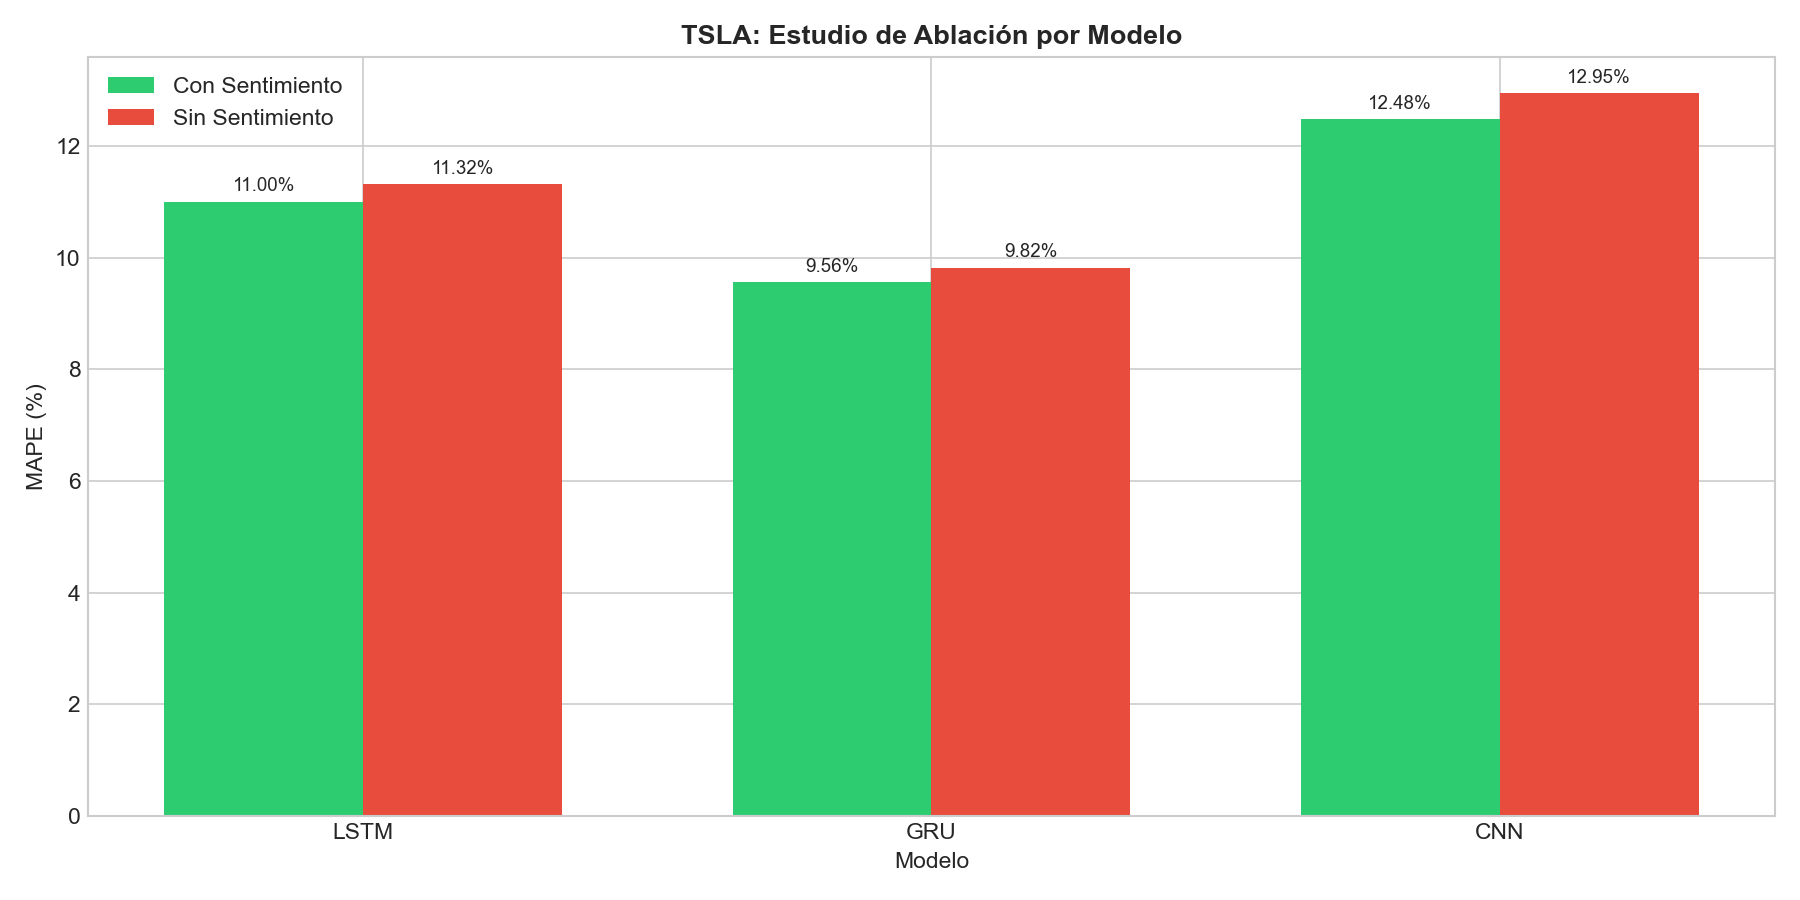
\includegraphics[width=0.90\textwidth]{Imagenes/ablation_TSLA_all_models.png}
\caption{TSLA: Ablación por modelo. Incluir sentimiento reduce el MAPE en los tres modelos, con mejoras pequeñas ($\sim$2--4\%).}
\label{fig:ablation_tsla}
\end{figure}

\begin{figure}[H]
\centering
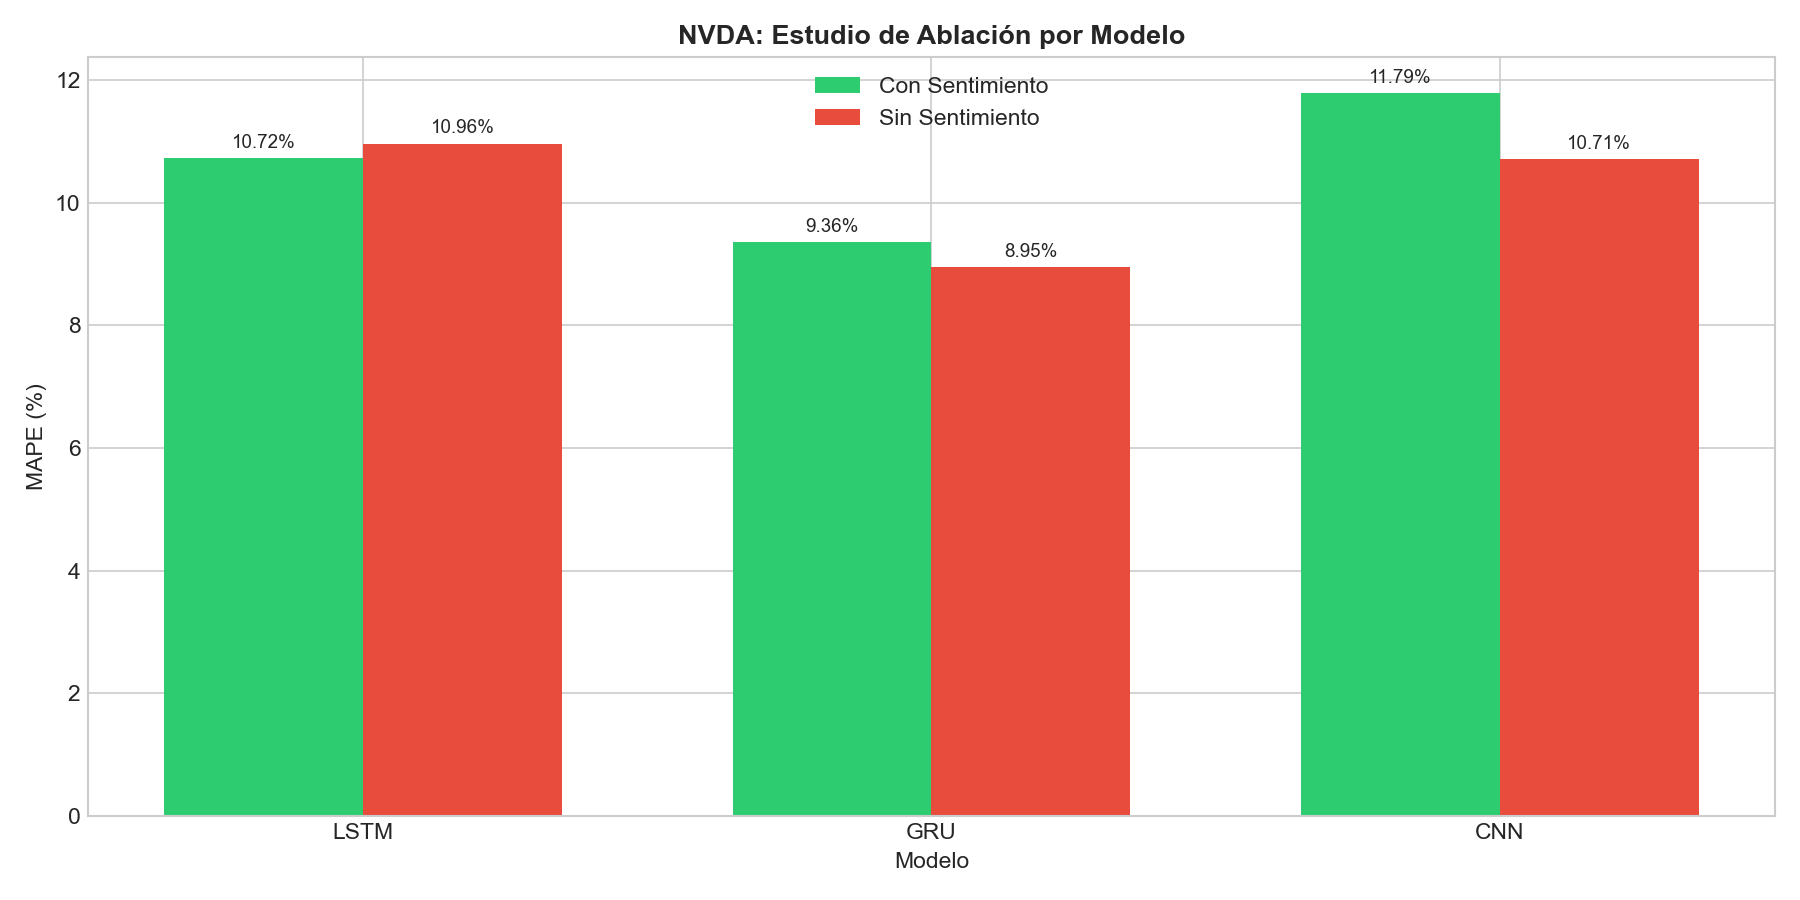
\includegraphics[width=0.90\textwidth]{Imagenes/ablation_NVDA_all_models.png}
\caption{NVDA: Ablación por modelo. LSTM mejora ligeramente; CNN y GRU empeoran.}
\label{fig:ablation_nvda}
\end{figure}

\begin{figure}[H]
\centering
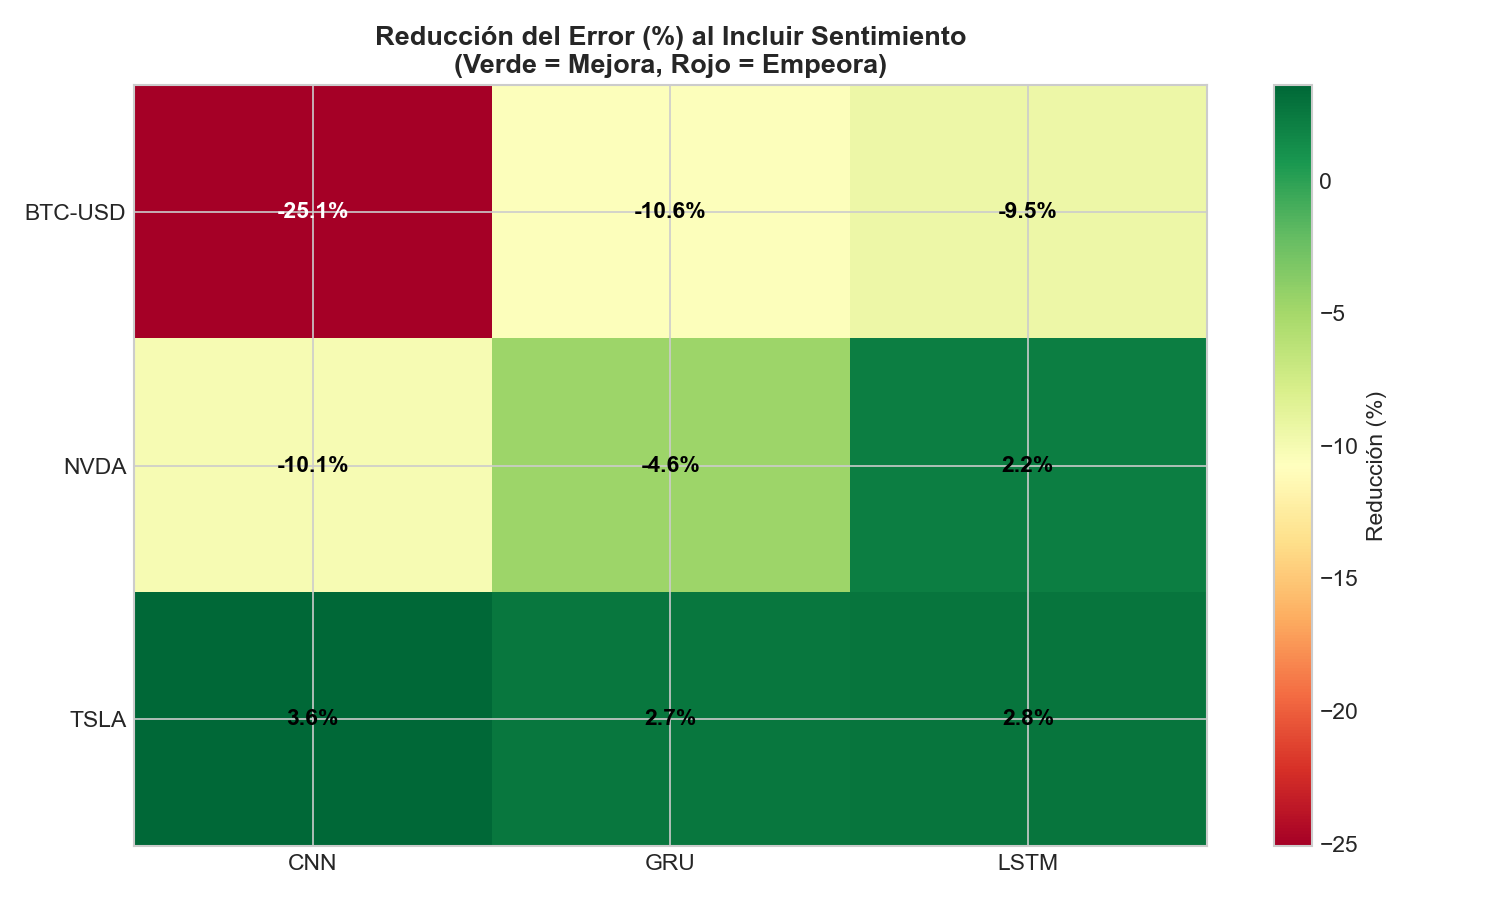
\includegraphics[width=0.90\textwidth]{Imagenes/ablation_improvement_heatmap.png}
\caption{Mapa de calor: Reducción del error (\%) al incluir sentimiento. Valores positivos (verdes) indican mejora; negativos (rojos) indican que el sentimiento perjudica.}
\label{fig:ablation_heatmap}
\end{figure}

Para ver el efecto desde el punto de vista de cada arquitectura, la Figura~\ref{fig:ablation_models_overview} resume la ablación por modelo en los tres activos.

\begin{figure}[H]
\centering
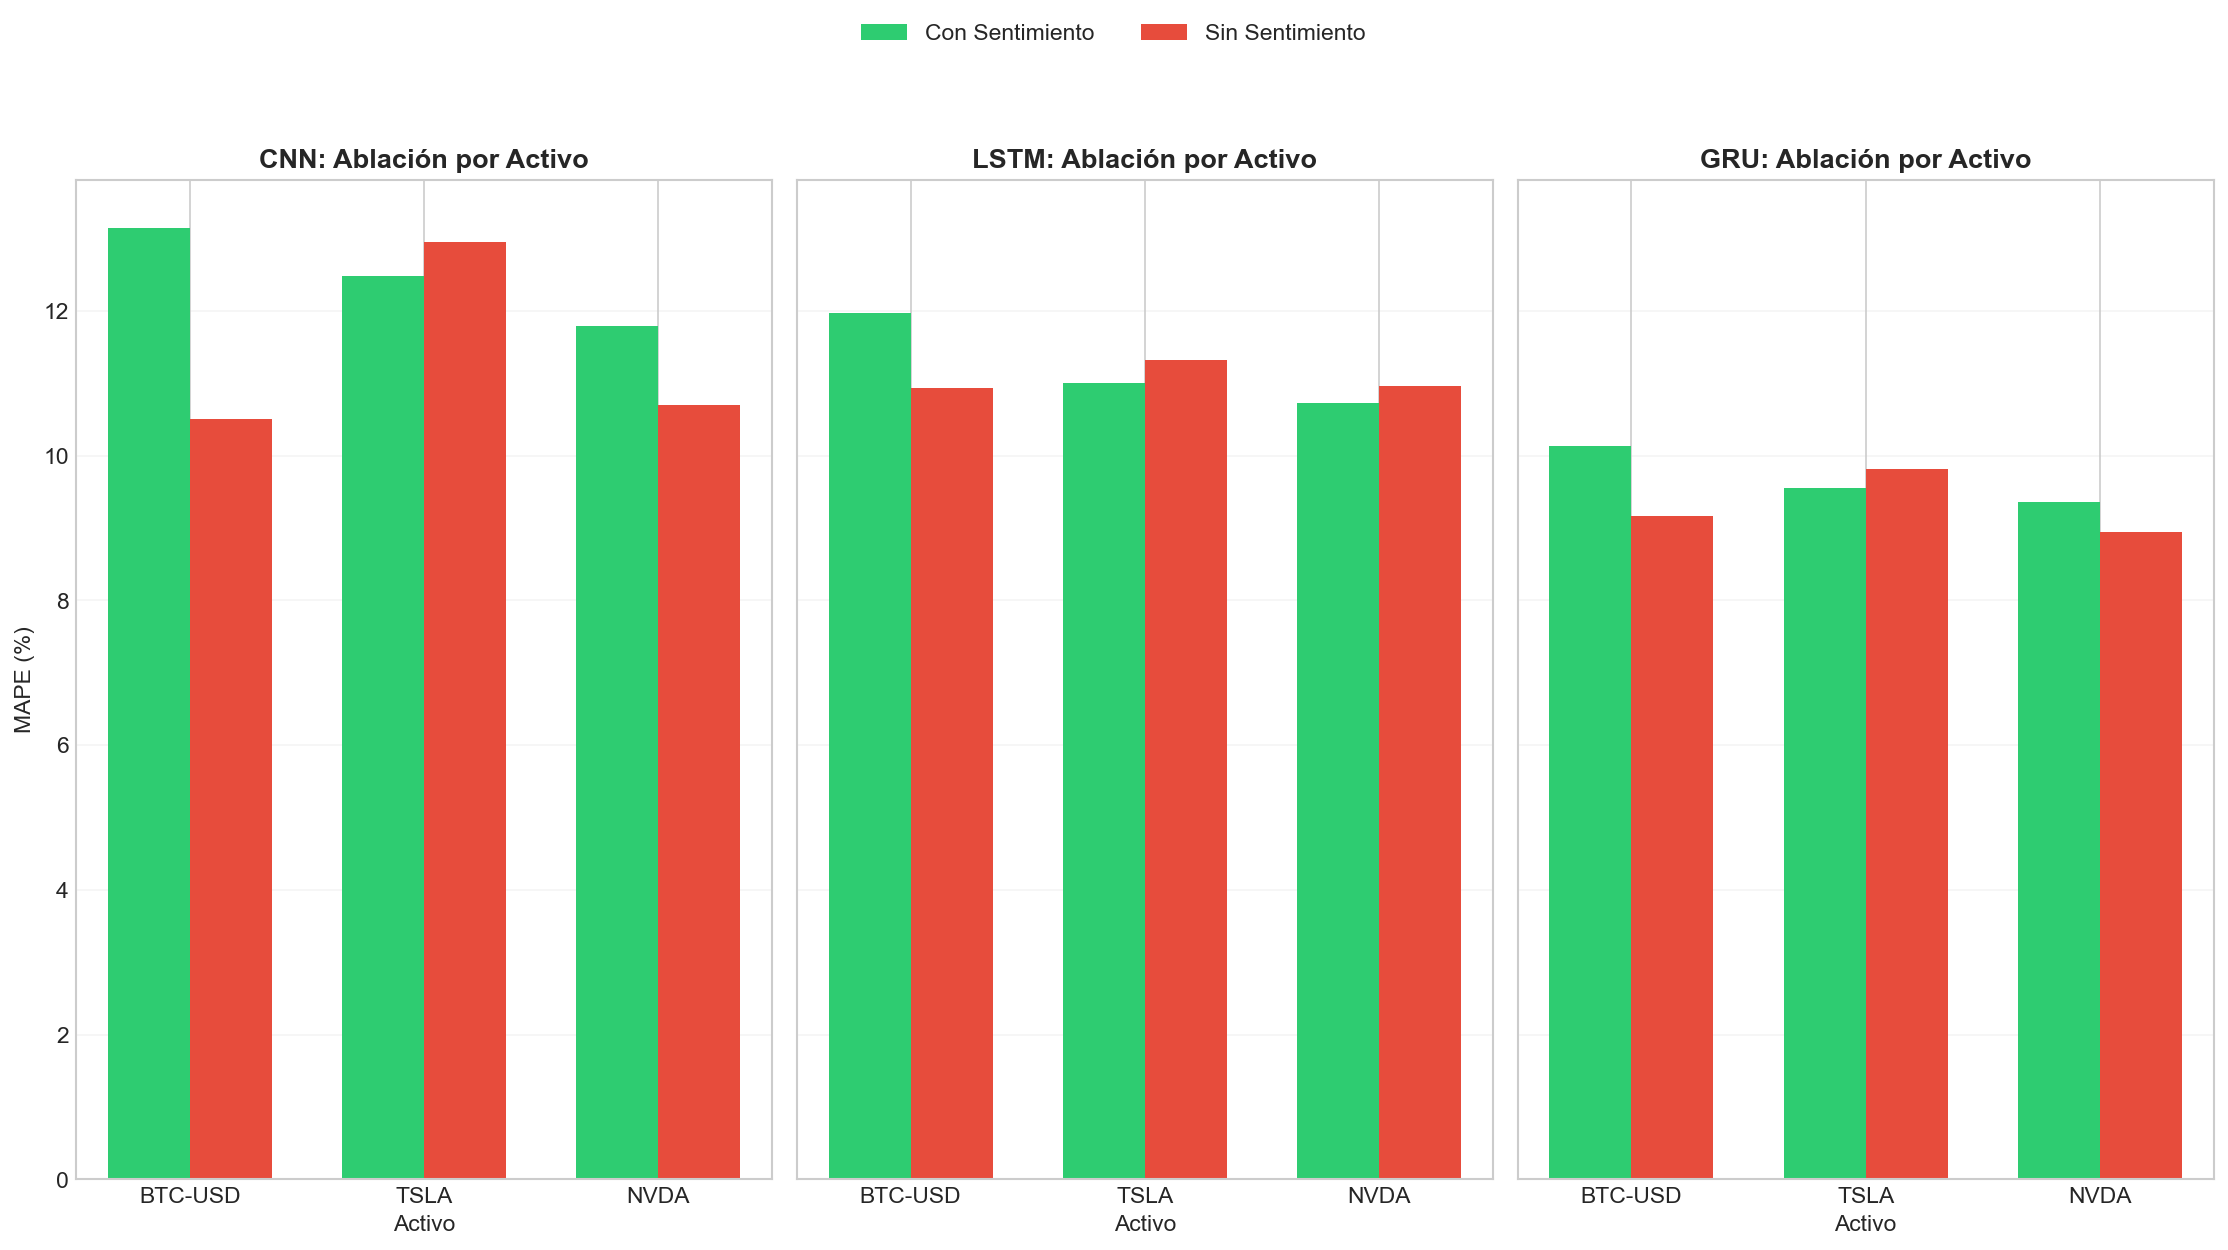
\includegraphics[width=0.95\textwidth]{Imagenes/ablation_models_overview.png}
\caption{Ablación por modelo (MAPE) comparando los tres activos.}
\label{fig:ablation_models_overview}
\end{figure}

En términos prácticos, esto significa que el sentimiento no es una ``mejora automática''. En Tesla aporta de forma consistente (aunque poco), mientras que en Bitcoin y, salvo en el caso de LSTM en Nvidia, tiende a perjudicar. La conclusión no es que el sentimiento carezca de utilidad, sino que su contribución se limita a determinadas condiciones.

\subsection{Significancia estadística de la ablación}

Además de comparar medias, se aplicó un test de Wilcoxon pareado sobre las métricas por fold para evaluar si la diferencia con/sin sentimiento es consistente. La Tabla~\ref{tab:ablation_tests} resume los resultados para MAPE y métricas direccionales (DA, F1 y MCC). En la tabla, la columna \textbf{Dif.} se define como \textbf{(sin sentimiento) $-$ (con sentimiento)}: en MAPE un valor positivo indica que incluir sentimiento reduce el error (mejora), mientras que en las métricas direccionales un valor positivo indica mejor comportamiento sin sentimiento.

\begin{table}[H]
\centering
\caption{Test de Wilcoxon para la ablación con/sin sentimiento}
\label{tab:ablation_tests}
\begin{tabular}{l|l|c|c|c|c}
\hline
\textbf{Activo} & \textbf{Modelo} & \textbf{Metr.} & \textbf{Dif.} & \textbf{p} & \textbf{Sig.?} \\
\hline
BTC-USD & CNN & MAPE & -2.64 & 0.233 & No \\
BTC-USD & GRU & MAPE & -0.97 & 1.000 & No \\
BTC-USD & LSTM & MAPE & -1.04 & 0.733 & No \\
NVDA & CNN & MAPE & -1.08 & 0.110 & No \\
NVDA & GRU & MAPE & -0.41 & 0.424 & No \\
NVDA & LSTM & MAPE & 0.24 & 0.470 & No \\
TSLA & CNN & MAPE & 0.47 & 0.380 & No \\
TSLA & GRU & MAPE & 0.26 & 0.470 & No \\
TSLA & LSTM & MAPE & 0.32 & 0.176 & No \\
BTC-USD & CNN & DA & 1.11 & 0.766 & No \\
BTC-USD & GRU & DA & 2.50 & 0.461 & No \\
BTC-USD & LSTM & DA & -1.94 & 0.688 & No \\
NVDA & CNN & DA & 2.50 & 0.508 & No \\
NVDA & GRU & DA & 0.56 & 1.000 & No \\
NVDA & LSTM & DA & -1.67 & 0.469 & No \\
TSLA & CNN & DA & -3.89 & 0.336 & No \\
TSLA & GRU & DA & 1.11 & 0.625 & No \\
TSLA & LSTM & DA & -0.28 & 0.844 & No \\
BTC-USD & CNN & F1 & 7.02 & 0.461 & No \\
BTC-USD & GRU & F1 & 7.37 & 0.164 & No \\
BTC-USD & LSTM & F1 & 3.03 & 0.742 & No \\
NVDA & CNN & F1 & 8.78 & 0.278 & No \\
NVDA & GRU & F1 & 1.07 & 0.812 & No \\
NVDA & LSTM & F1 & -3.11 & 0.461 & No \\
TSLA & CNN & F1 & -9.52 & 0.206 & No \\
TSLA & GRU & F1 & 2.21 & 0.312 & No \\
TSLA & LSTM & F1 & 0.68 & 0.688 & No \\
BTC-USD & CNN & MCC & -0.02 & 0.652 & No \\
BTC-USD & GRU & MCC & 0.00 & 0.910 & No \\
BTC-USD & LSTM & MCC & -0.00 & 0.742 & No \\
NVDA & CNN & MCC & 0.12 & 0.024 & Si \\
NVDA & GRU & MCC & -0.03 & 0.812 & No \\
NVDA & LSTM & MCC & 0.01 & 0.945 & No \\
TSLA & CNN & MCC & -0.08 & 0.465 & No \\
TSLA & GRU & MCC & 0.03 & 0.688 & No \\
TSLA & LSTM & MCC & 0.05 & 0.297 & No \\
\hline
\end{tabular}
\end{table}

La Figura~\ref{fig:wilcoxon_pvalues} ofrece una lectura rápida de los p-values: cuanto más oscuro, más evidencia contra la hipótesis nula.

\begin{figure}[H]
\centering
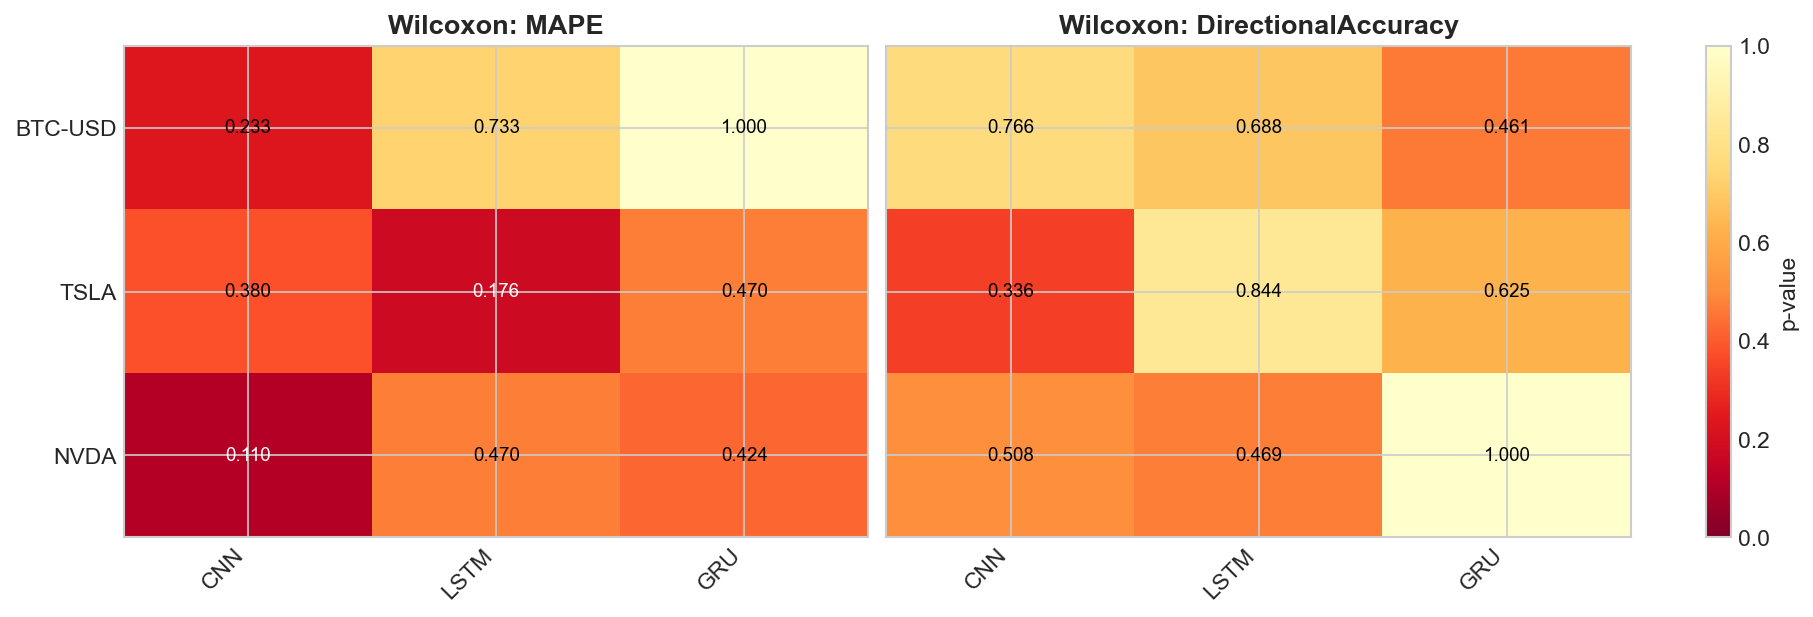
\includegraphics[width=0.95\textwidth]{Imagenes/wilcoxon_pvalues_heatmap.png}
\caption{P-values del test de Wilcoxon para MAPE y precisión direccional.}
\label{fig:wilcoxon_pvalues}
\end{figure}

En MAPE y en DA/F1 no aparecen diferencias significativas (p < 0.05) en ninguna combinación. Solo aparece un caso aislado significativo en MCC (NVDA-CNN), por lo que no cambia la conclusión general. El signo de \textbf{Dif.} sugiere tendencias (por ejemplo, que el sentimiento tiende a empeorar el MAPE en Bitcoin y a mejorar ligeramente en Tesla), pero el efecto no es estadísticamente consistente por fold.

En síntesis, no hay evidencia sólida de que el error baje de forma repetible al incluir sentimiento. Eso pone límites a cualquier conclusión contundente y es coherente con la variabilidad que se observa en la ablación.

Implicación práctica: incluir sentimiento tiene un coste (datos y procesamiento) y solo se justifica cuando la mejora es clara, estable y repetible. En este estudio, aunque Tesla muestra un patrón favorable, el tamaño del efecto es pequeño y no alcanza significancia estadística.

%% ============================================================
%% EXPERIMENTO D: PERIODOS DE MERCADO
%% ============================================================

\section{Rendimiento por periodos de mercado}

El último experimento compara el rendimiento de los tres modelos de aprendizaje profundo (LSTM, GRU y CNN) en tres periodos muy diferentes para Bitcoin.

\subsection{Los números}

La Tabla~\ref{tab:experiment_d} recoge las métricas de cada modelo en los tres periodos, y la Figura~\ref{fig:market_periods} las visualiza.

\begin{table}[H]
\centering
\caption{Rendimiento de LSTM, GRU y CNN por periodo de mercado (BTC-USD, h=7)}
\label{tab:experiment_d}
\begin{tabular}{l|l|ccc}
\hline
\textbf{Periodo} & \textbf{Modelo} & \textbf{RMSE (USD)} & \textbf{MAE (USD)} & \textbf{MAPE (\%)} \\
\hline
Bull-2021 & LSTM & 8513 & 7184 & 11.99 \\
Bull-2021 & GRU & 6336 & 5165 & 8.71 \\
Bull-2021 & CNN & 9405 & 7577 & 12.64 \\
Bear-2022 & LSTM & 1571 & 1143 & 6.50 \\
Bear-2022 & GRU & 1816 & 1368 & 7.41 \\
Bear-2022 & CNN & 1642 & 1258 & 7.13 \\
Recent & LSTM & 6868 & 5451 & 4.86 \\
Recent & GRU & 5180 & 4085 & 3.71 \\
Recent & CNN & 8482 & 7050 & 6.48 \\
\hline
\end{tabular}
\end{table}

\begin{figure}[H]
\centering
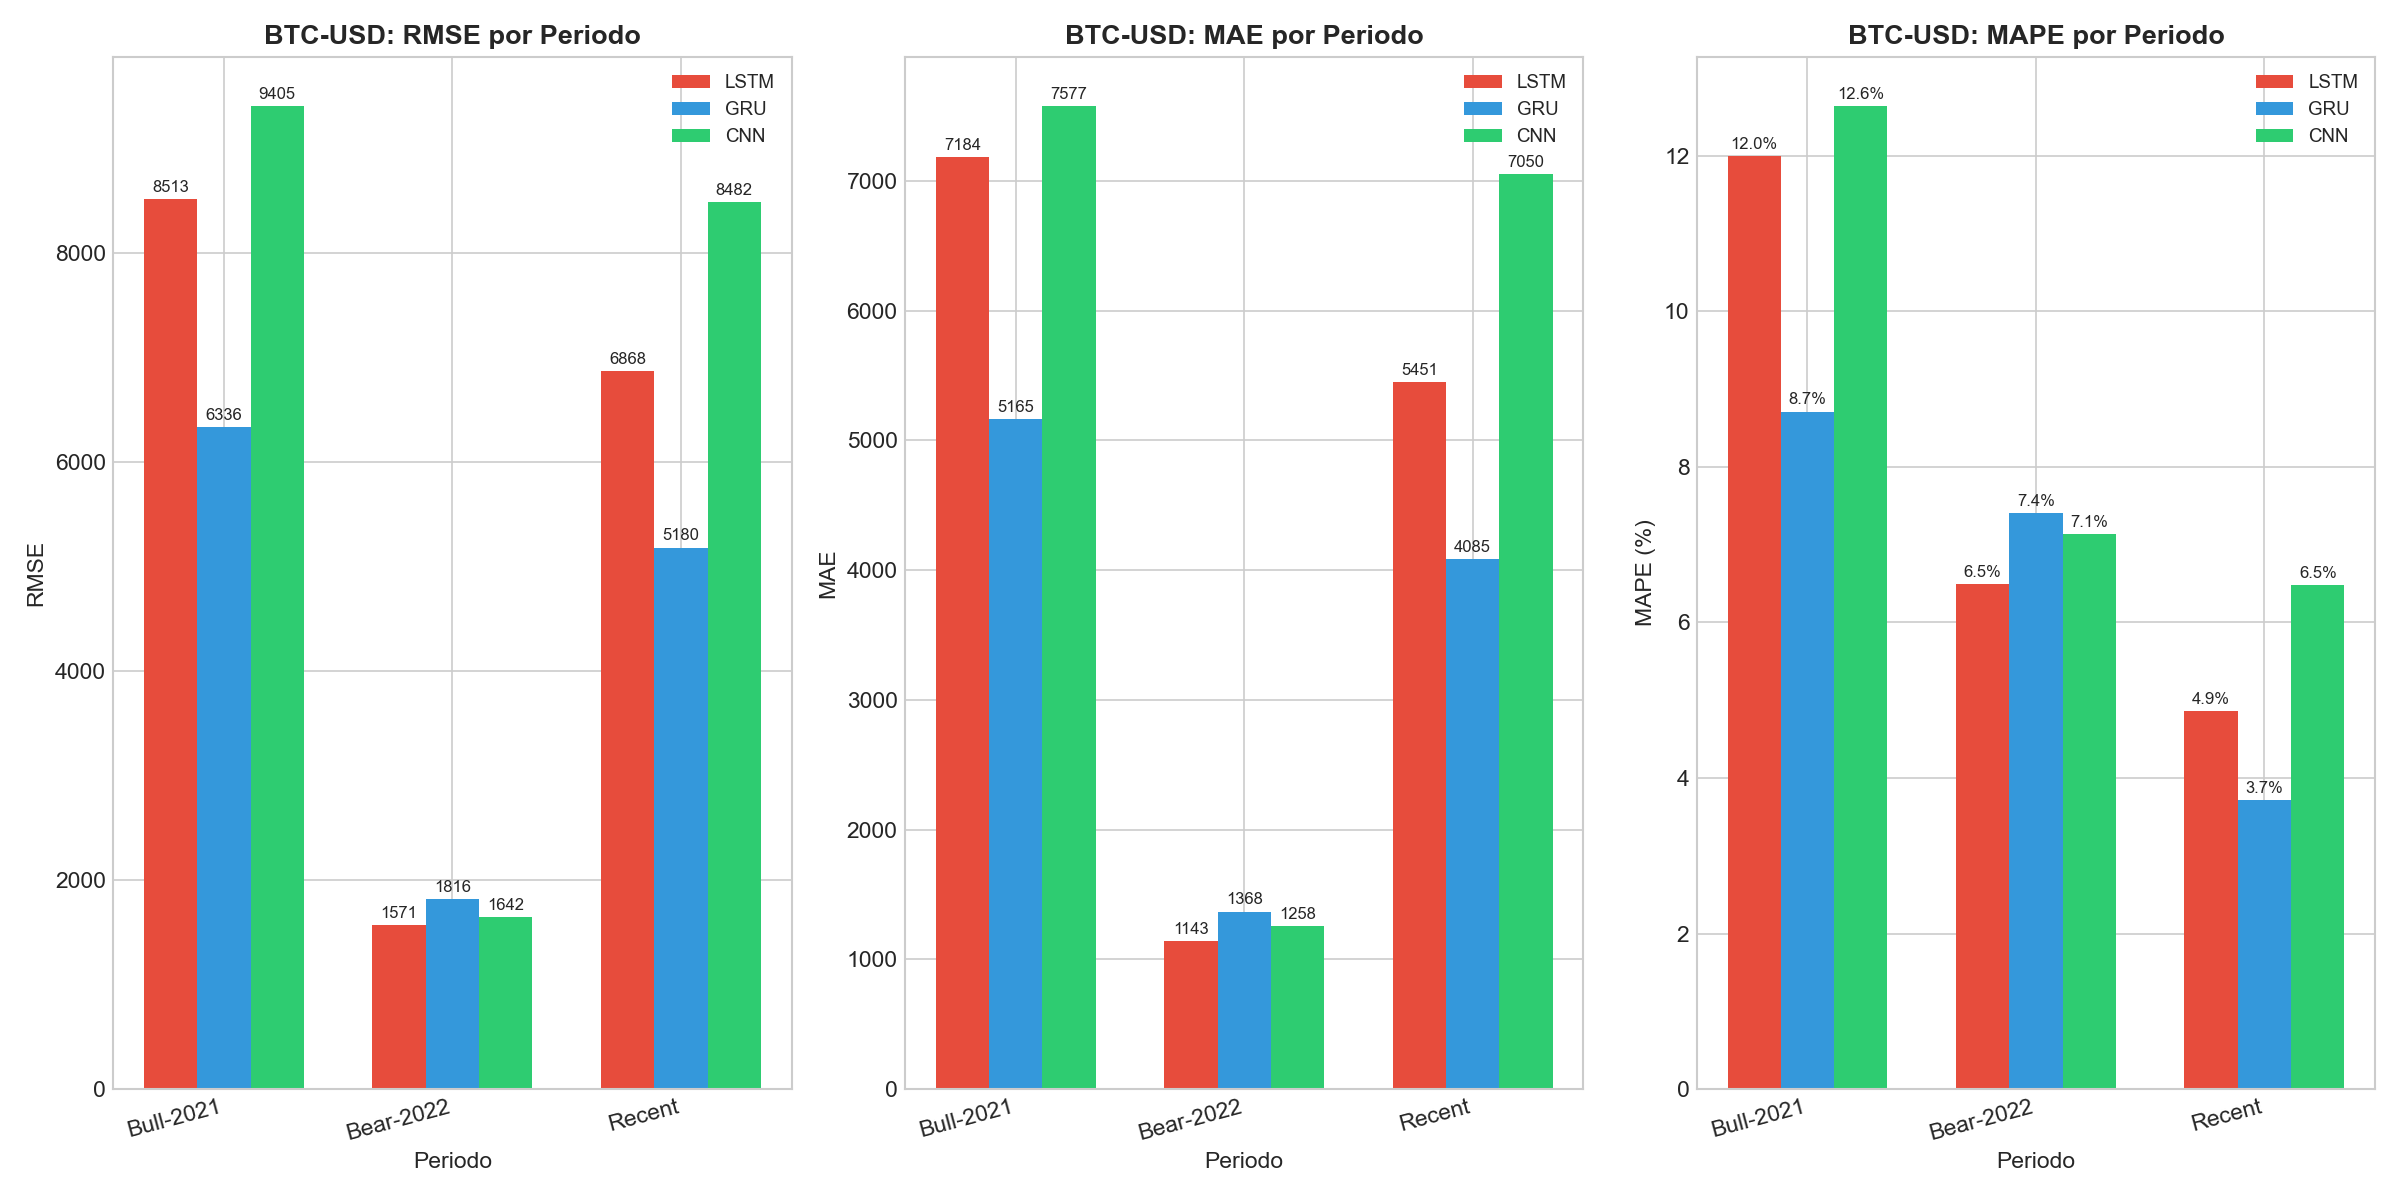
\includegraphics[width=0.95\textwidth]{Imagenes/market_periods_all_metrics.png}
\caption{Rendimiento por periodo de mercado para los tres modelos DL.}
\label{fig:market_periods}
\end{figure}

El rendimiento varía sustancialmente entre periodos y entre modelos. En el periodo alcista de 2021, GRU es claramente el mejor modelo (MAPE 8.71\%), mientras que LSTM (11.99\%) y CNN (12.64\%) quedan lejos. En el mercado bajista de 2022, las diferencias se reducen: LSTM obtiene el menor MAPE (6.50\%), seguido de CNN (7.13\%) y GRU (7.41\%). En el periodo reciente, GRU vuelve a liderar con un MAPE de 3.71\%, seguido de LSTM (4.86\%) y CNN (6.48\%).

Este resultado tiene varias lecturas. Primero, GRU es la arquitectura más consistente en dos de los tres periodos y la que mejor MAPE global presenta. Segundo, respecto al tramo alcista de 2021, el rendimiento en el mercado bajista de 2022 mejora para los tres modelos en MAPE, lo que puede parecer contraintuitivo; sin embargo, los precios absolutos eran significativamente menores, lo que reduce el error relativo. Tercero, CNN muestra una consistencia intermedia pero es la más inestable en direccionalidad: en el periodo reciente apenas alcanza un 37.5\% de precisión direccional, lo que es peor que el azar.

Por tanto, el rendimiento de un mismo modelo puede variar sustancialmente entre periodos, incluso con hiperparámetros constantes. Esta sensibilidad al régimen es una limitación práctica que conviene explicitar. Además, las diferencias entre arquitecturas se amplifican en ciertos regímenes, lo que sugiere que la elección del modelo no es independiente del contexto de mercado.

Implicación práctica: si se usa un modelo para apoyar decisiones, hay que vigilar el contexto de mercado y considerar que el ranking entre LSTM, GRU y CNN puede cambiar según el régimen. GRU parece la opción más segura como punto de partida, pero LSTM puede superarlo en entornos bajistas.

%% ============================================================
%% PREDICCIONES VS VALORES REALES
%% ============================================================

\section{Análisis cualitativo de predicciones}

Las tablas resumen métricas agregadas, mientras que las figuras permiten evaluar la dinámica del ajuste. En esta sección se muestran las predicciones superpuestas con los valores reales para cada activo y horizonte.

La idea no es buscar coincidencia punto a punto, sino ver si el modelo sigue la tendencia general y qué tipo de errores comete: desfases, suavizado de picos o incapacidad para reaccionar a shocks.

Estas gráficas se generan con el conjunto completo de variables, incluyendo sentimiento; es decir, corresponden a la versión ``con sentimiento'' del modelo.

\subsection{Bitcoin}

\begin{figure}[H]
\centering
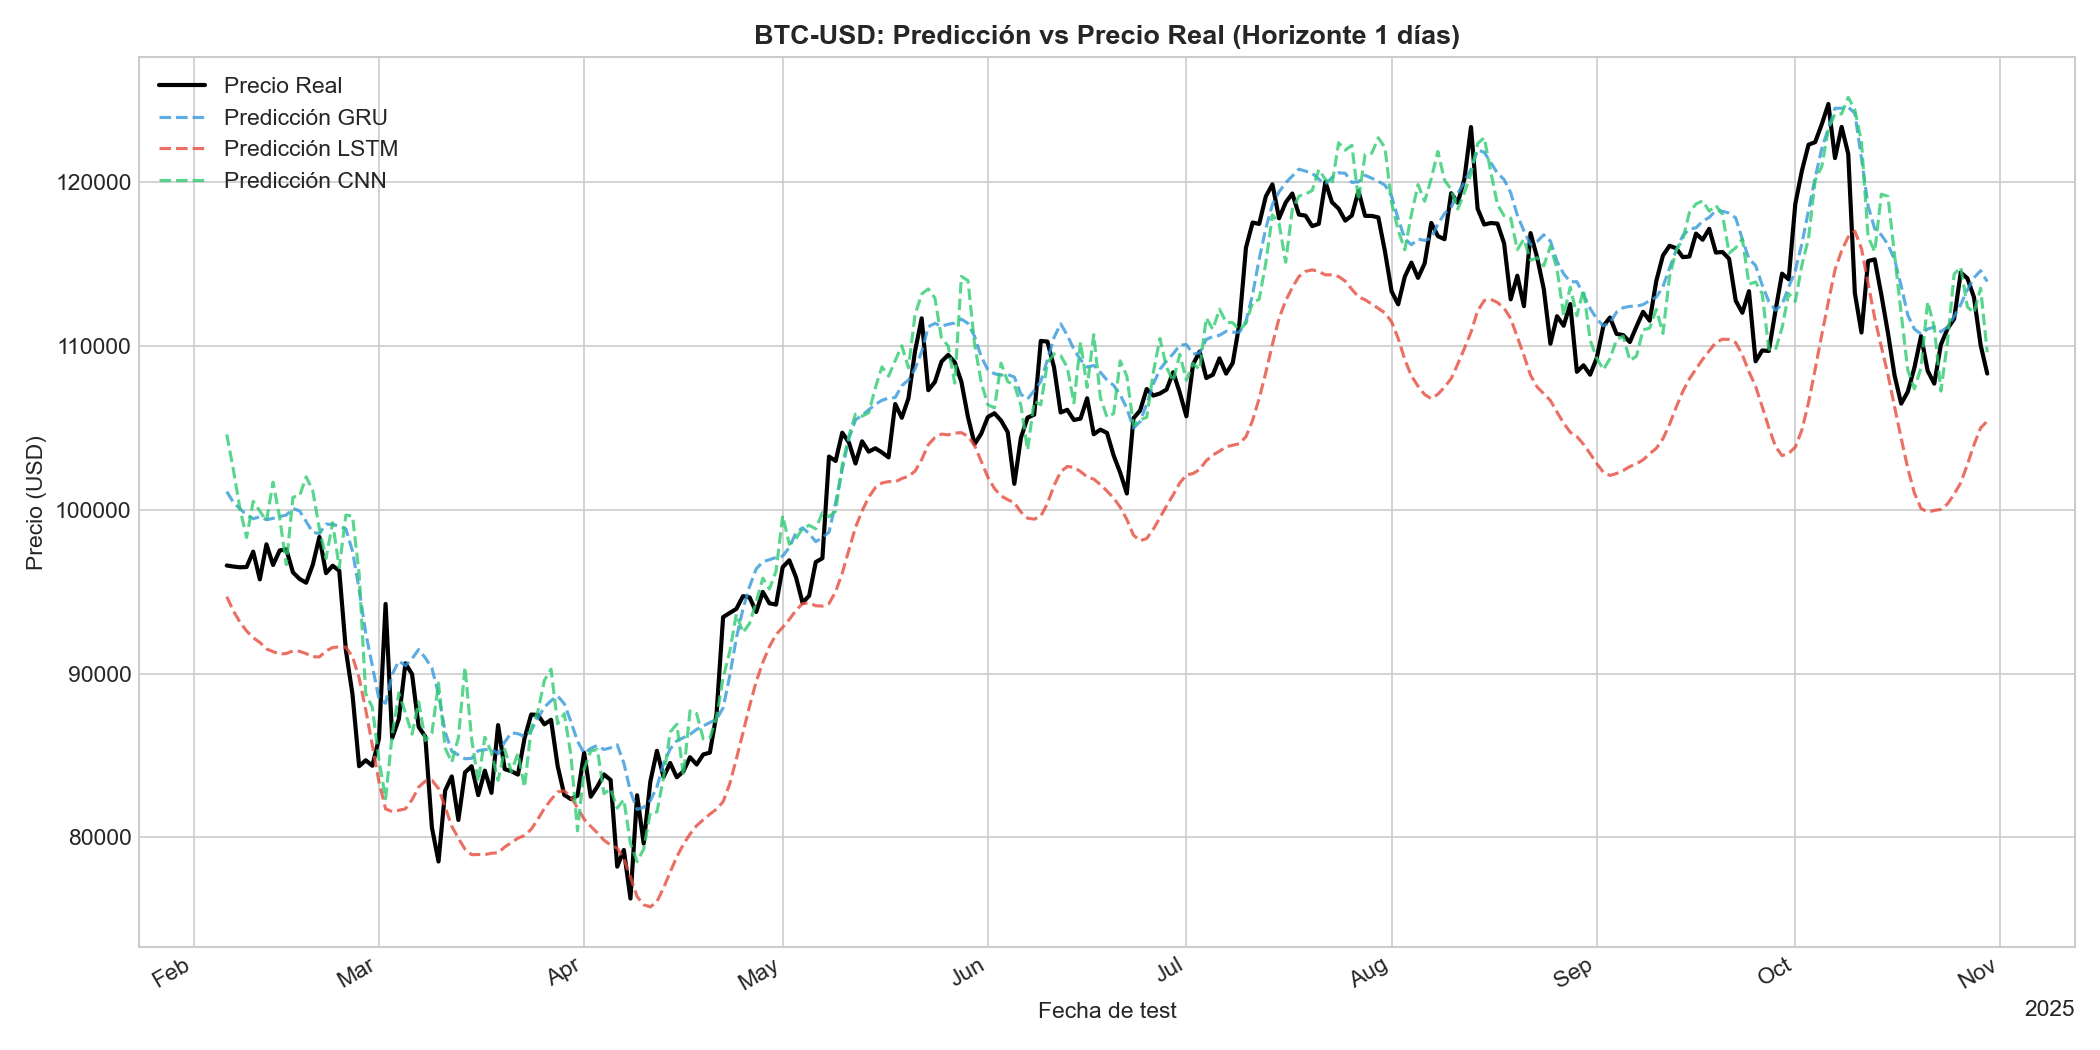
\includegraphics[width=0.95\textwidth]{Imagenes/pred_vs_actual_BTC_USD_h1.png}
\caption{BTC-USD: Predicción vs Real (1 día). A horizonte de un día, el modelo sigue de cerca la serie real, aunque con un ligero retardo. Las predicciones tienden a suavizar los picos, lo que es típico de modelos que aprenden de ventanas históricas.}
\label{fig:pred_btc_h1}
\end{figure}

\begin{figure}[H]
\centering
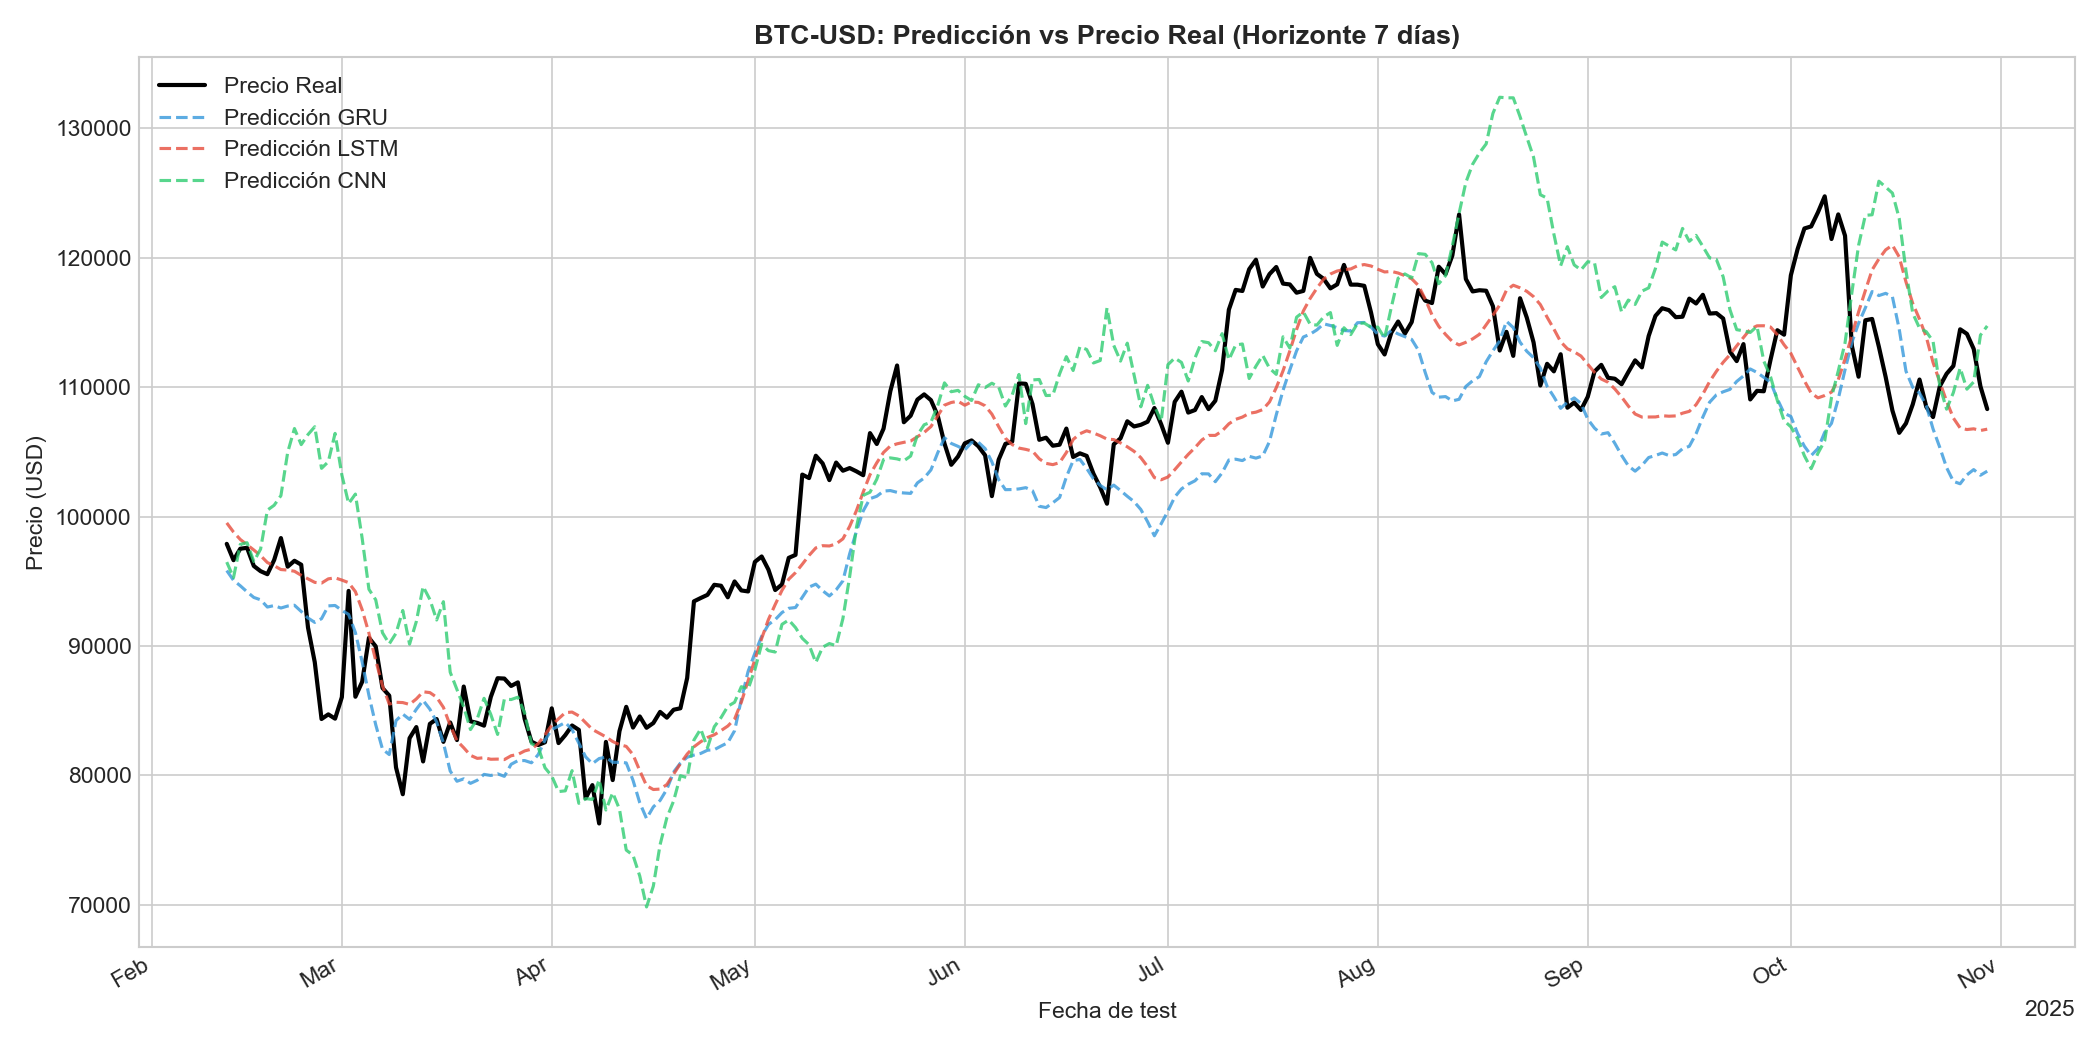
\includegraphics[width=0.95\textwidth]{Imagenes/pred_vs_actual_BTC_USD_h7.png}
\caption{BTC-USD: Predicción vs Real (7 días). Con una semana de horizonte, el error aumenta pero la tendencia general sigue siendo reconocible. Los cambios bruscos de dirección son los que mayor error generan, ya que el modelo no puede anticipar eventos inesperados.}
\label{fig:pred_btc_h7}
\end{figure}

\begin{figure}[H]
\centering
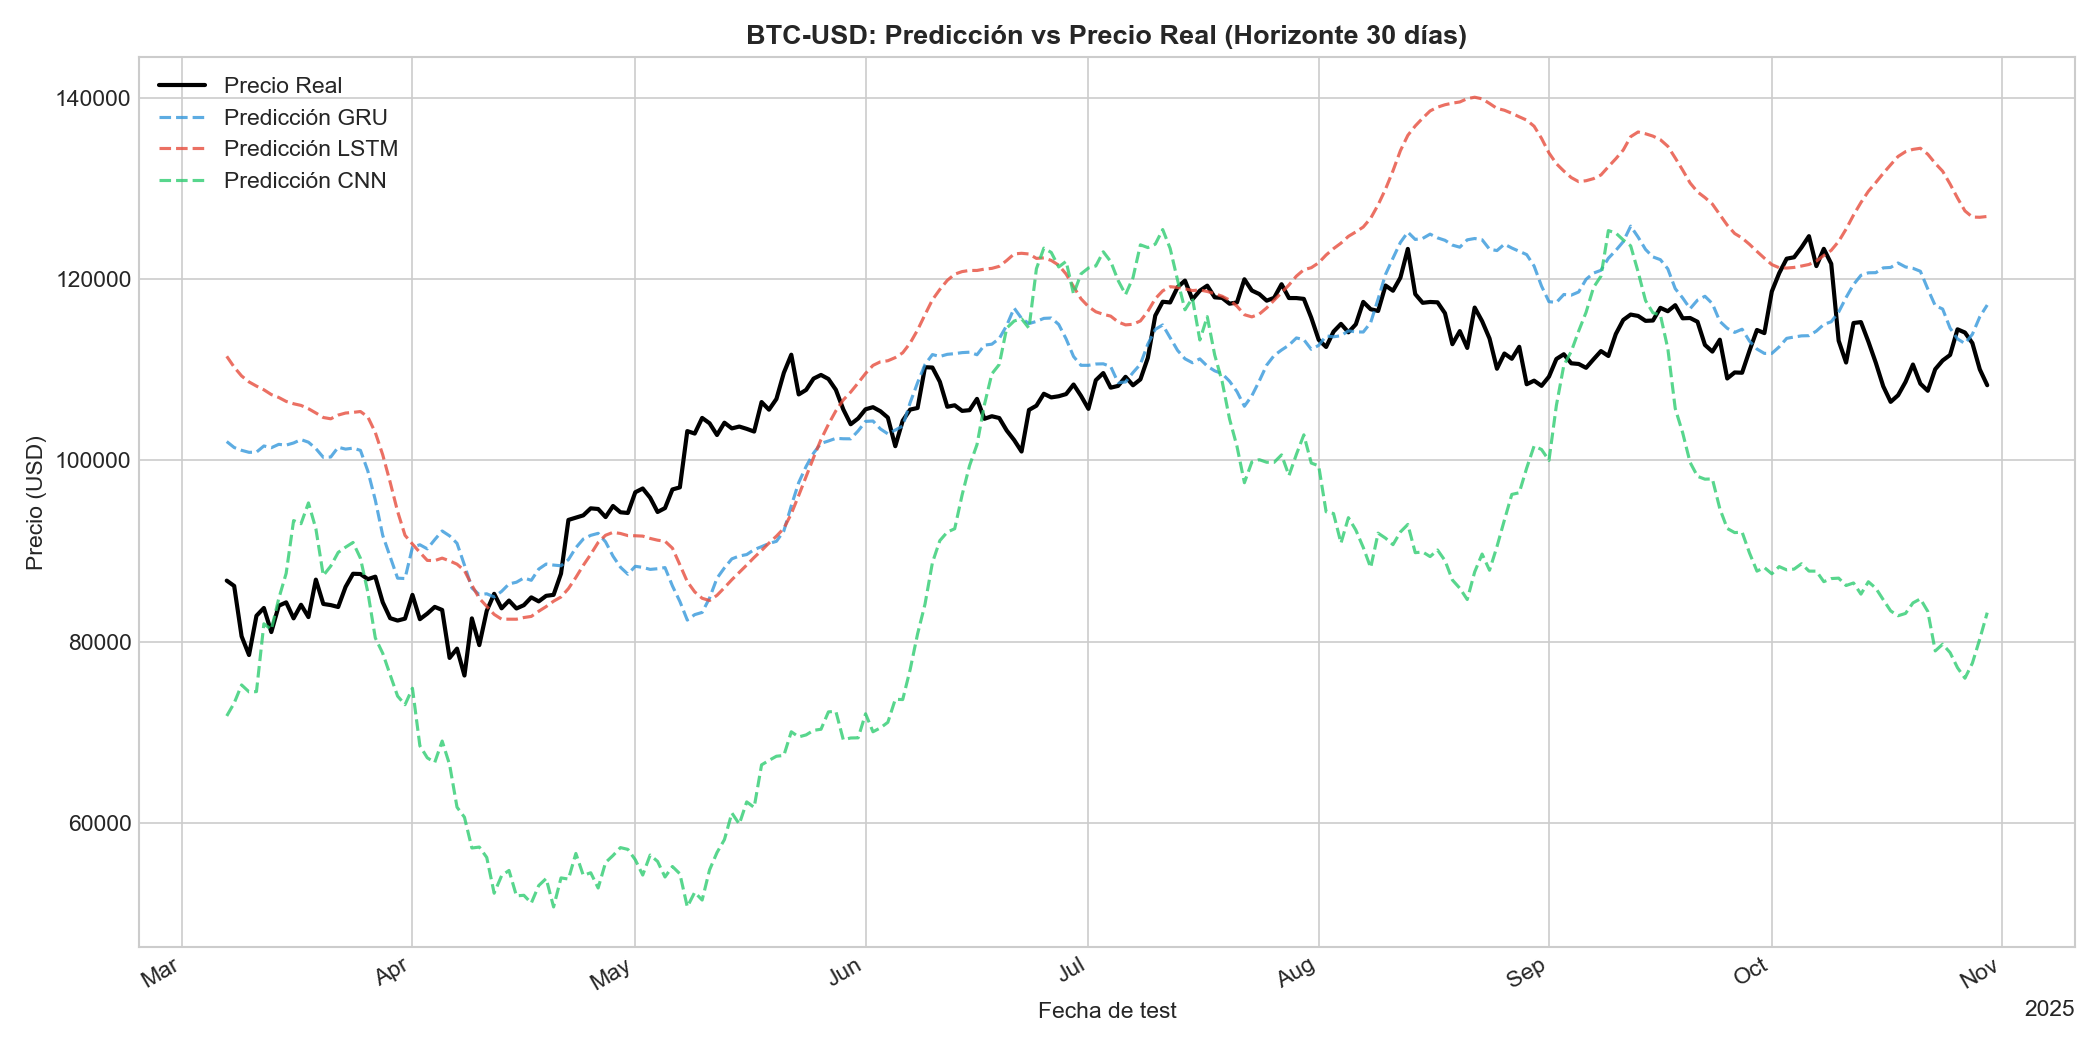
\includegraphics[width=0.95\textwidth]{Imagenes/pred_vs_actual_BTC_USD_h30.png}
\caption{BTC-USD: Predicción vs Real (30 días). A un mes, la predicción se convierte esencialmente en una media suavizada. El modelo captura la dirección general pero pierde resolución en los movimientos intermedios.}
\label{fig:pred_btc_h30}
\end{figure}

En conjunto, las gráficas de Bitcoin muestran un patrón consistente: las predicciones tienden a suavizar los movimientos y a llegar tarde a los cambios bruscos. Esto es habitual en modelos entrenados con ventanas históricas y refleja la dificultad intrínseca de anticipar shocks en un mercado tan volátil como el de criptomonedas. A medida que aumenta el horizonte, la curva de predicción se aplana progresivamente, lo que indica que el modelo pierde capacidad de seguimiento y converge hacia valores medios.

\clearpage
\subsection{Tesla}

\begin{figure}[H]
\centering
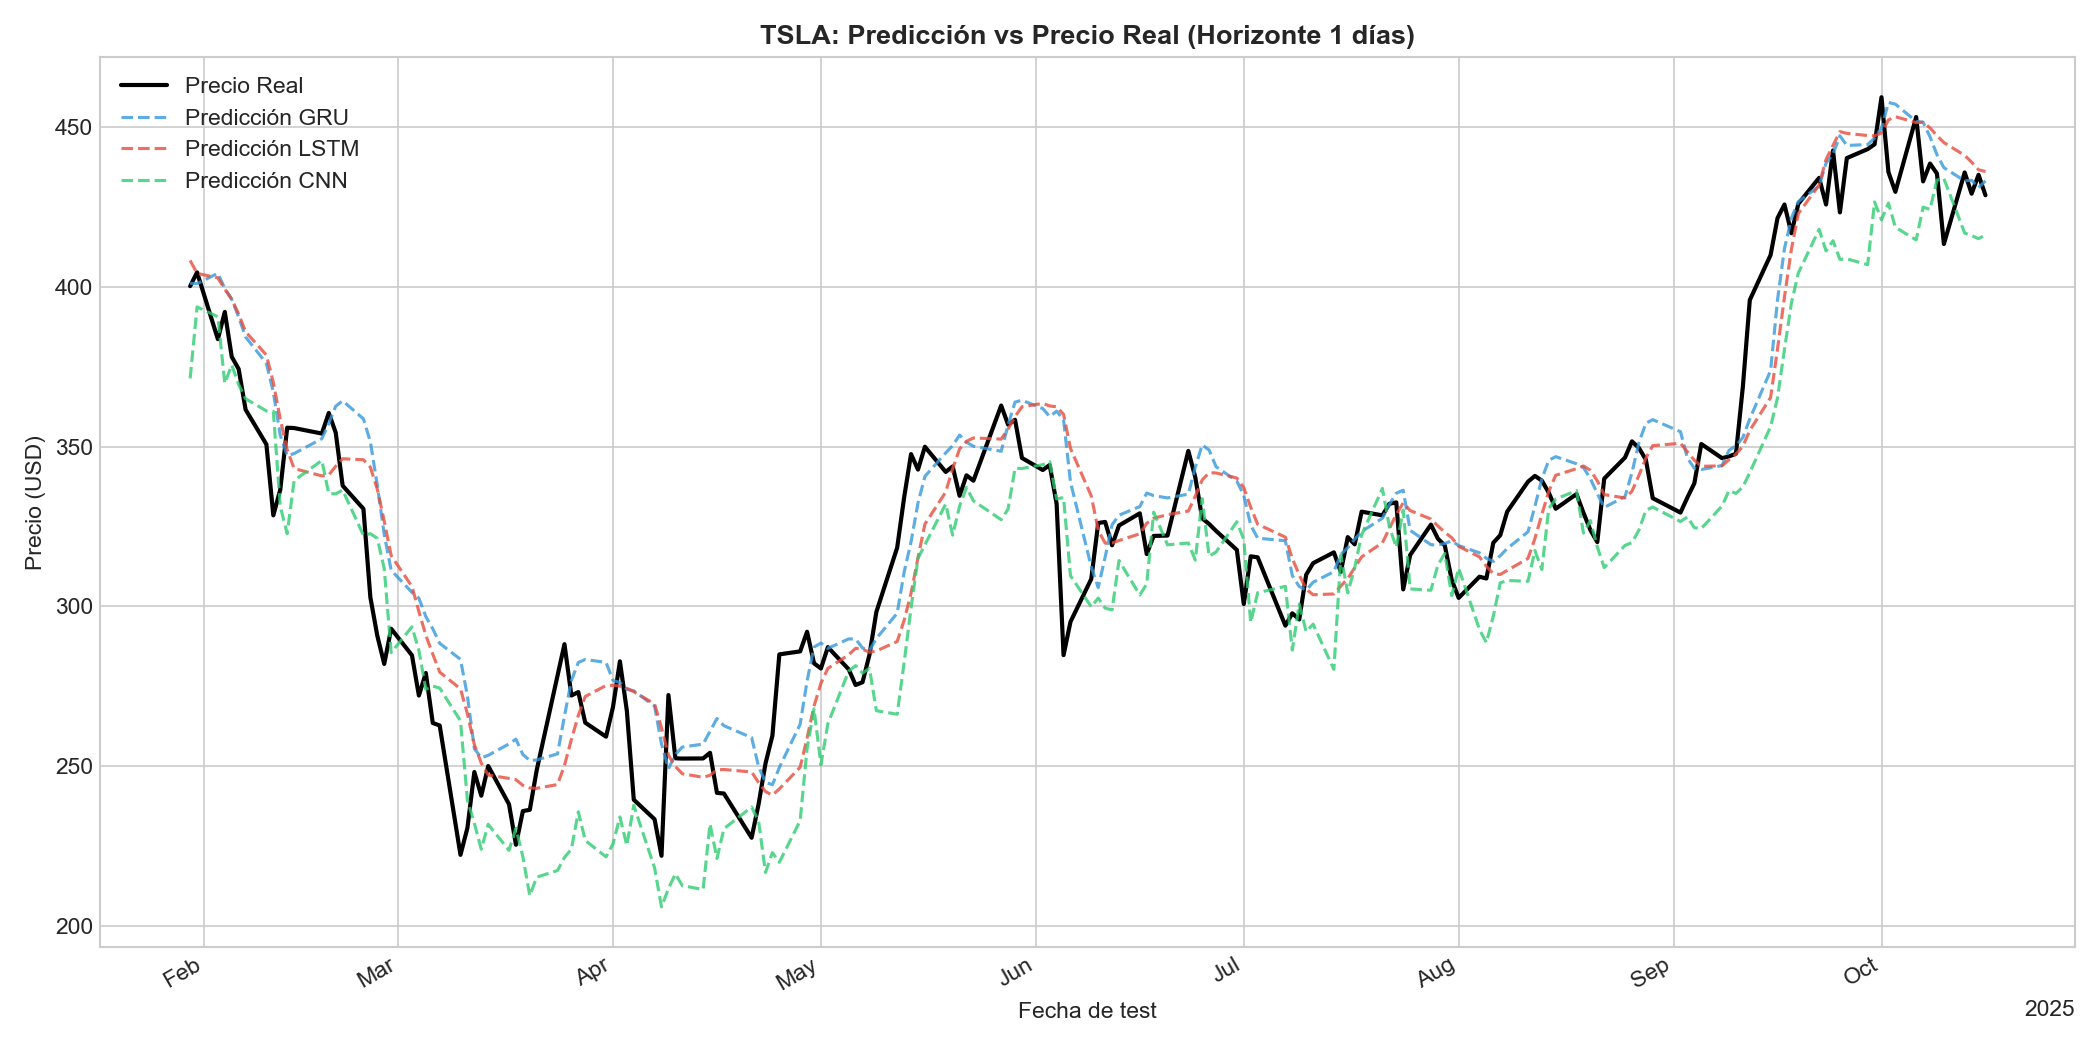
\includegraphics[width=0.95\textwidth]{Imagenes/pred_vs_actual_TSLA_h1.png}
\caption{TSLA: Predicción vs Real (1 día). Tesla muestra un ajuste visual más limpio que Bitcoin a corto plazo. El modelo captura la mayoría de movimientos diarios, aunque tiende a subestimar la magnitud de los picos más pronunciados.}
\label{fig:pred_tsla_h1}
\end{figure}

\begin{figure}[H]
\centering
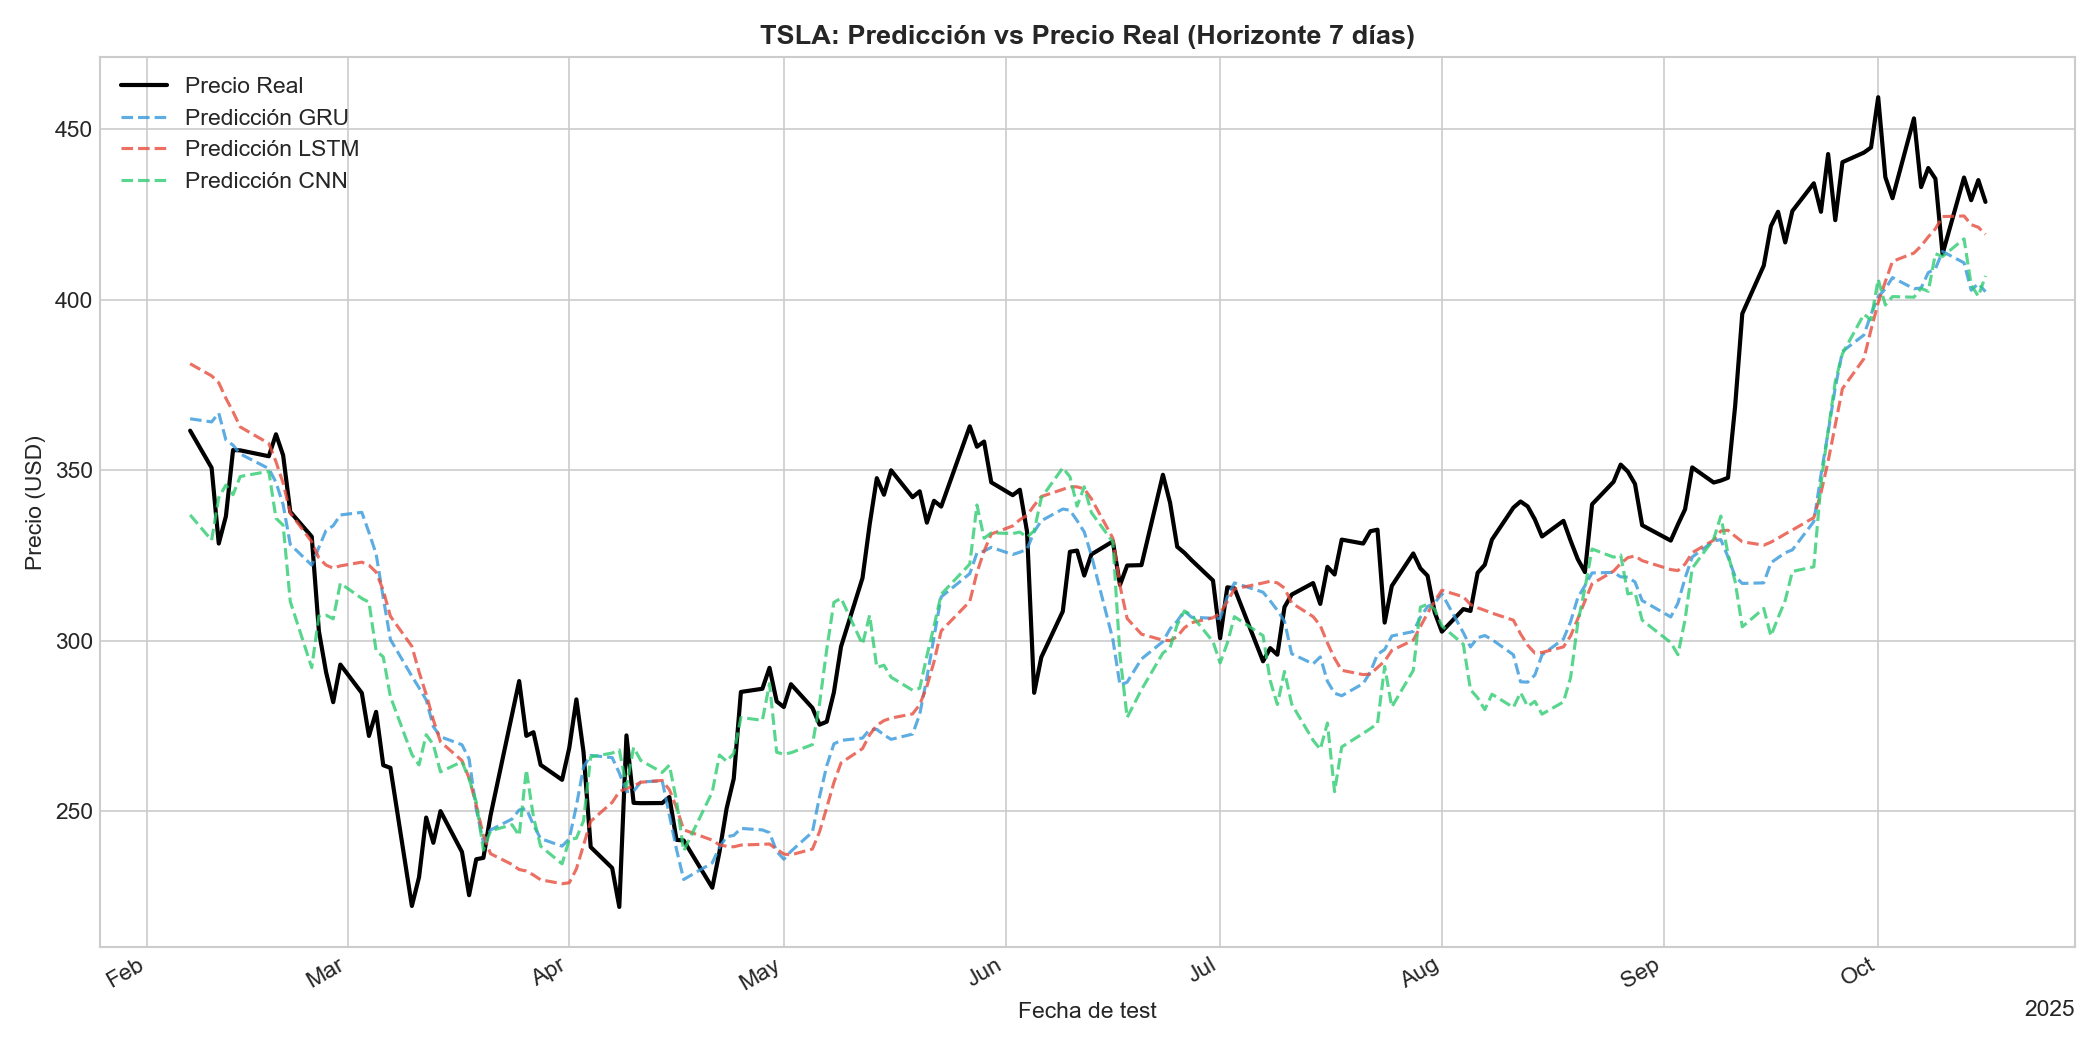
\includegraphics[width=0.95\textwidth]{Imagenes/pred_vs_actual_TSLA_h7.png}
\caption{TSLA: Predicción vs Real (7 días). A una semana, el modelo mantiene un seguimiento razonable de la tendencia, aunque los picos de volatilidad generan desviaciones significativas. Los periodos de baja volatilidad muestran mejor ajuste que los turbulentos.}
\label{fig:pred_tsla_h7}
\end{figure}

\begin{figure}[H]
\centering
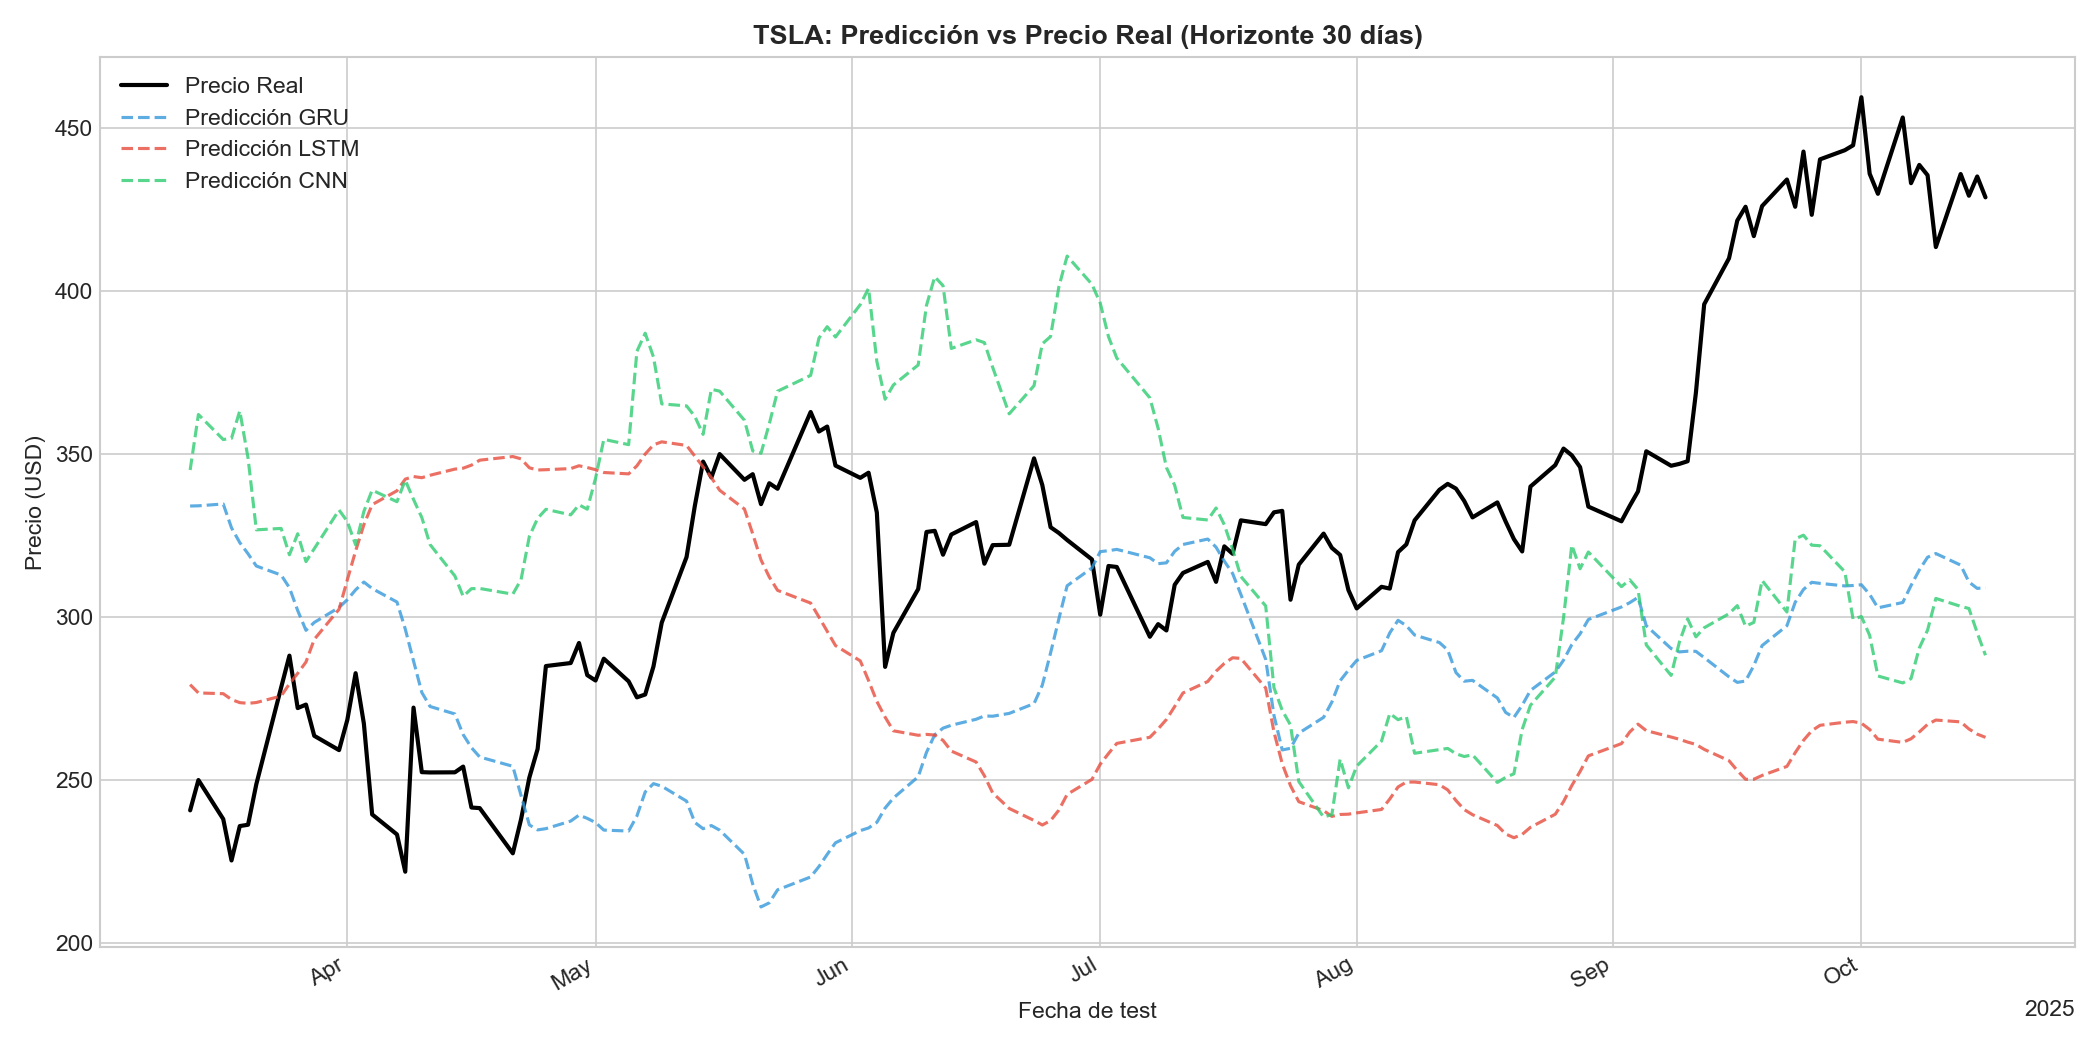
\includegraphics[width=0.95\textwidth]{Imagenes/pred_vs_actual_TSLA_h30.png}
\caption{TSLA: Predicción vs Real (30 días). Con horizonte de un mes, las predicciones capturan la tendencia general pero pierden precisión en los movimientos intermedios. Los cambios de régimen (por ejemplo, tras earnings o noticias de Elon Musk) son especialmente difíciles de anticipar.}
\label{fig:pred_tsla_h30}
\end{figure}

En conjunto, Tesla presenta una evolución más estable que Bitcoin en horizontes cortos en estas gráficas, pero un buen ajuste visual no implica necesariamente mejor MAPE: en la comparación global a 7 días, los baselines siguen siendo los modelos con menor error. Además, aunque el estudio de ablación sugiere una mejora ligera al incluir sentimiento en TSLA, el efecto no es estadísticamente significativo.

\clearpage
\subsection{Nvidia}

\begin{figure}[H]
\centering
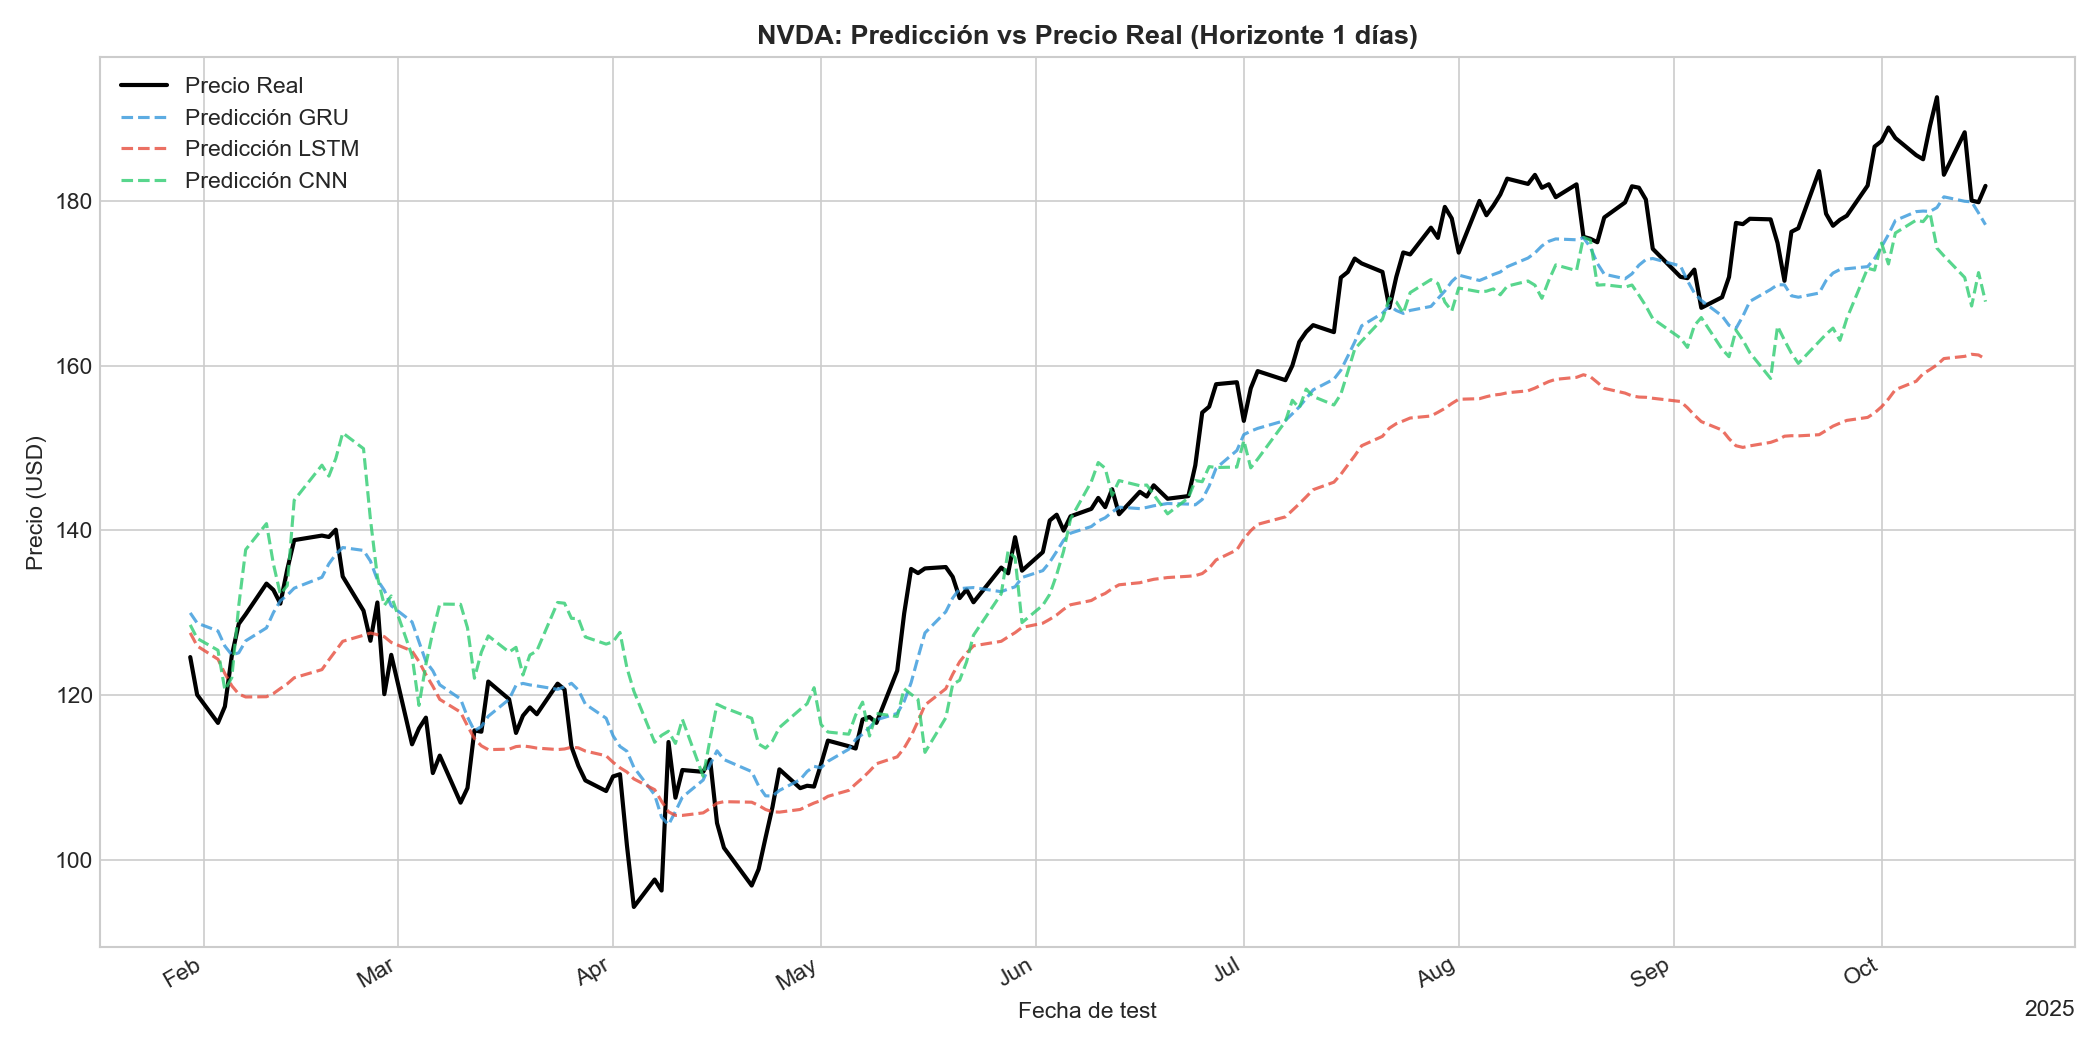
\includegraphics[width=0.95\textwidth]{Imagenes/pred_vs_actual_NVDA_h1.png}
\caption{NVDA: Predicción vs Real (1 día). Nvidia muestra un seguimiento cercano de la tendencia a corto plazo. Las oscilaciones diarias están bien capturadas, aunque con el típico retardo de los modelos basados en ventanas históricas.}
\label{fig:pred_nvda_h1}
\end{figure}

\begin{figure}[H]
\centering
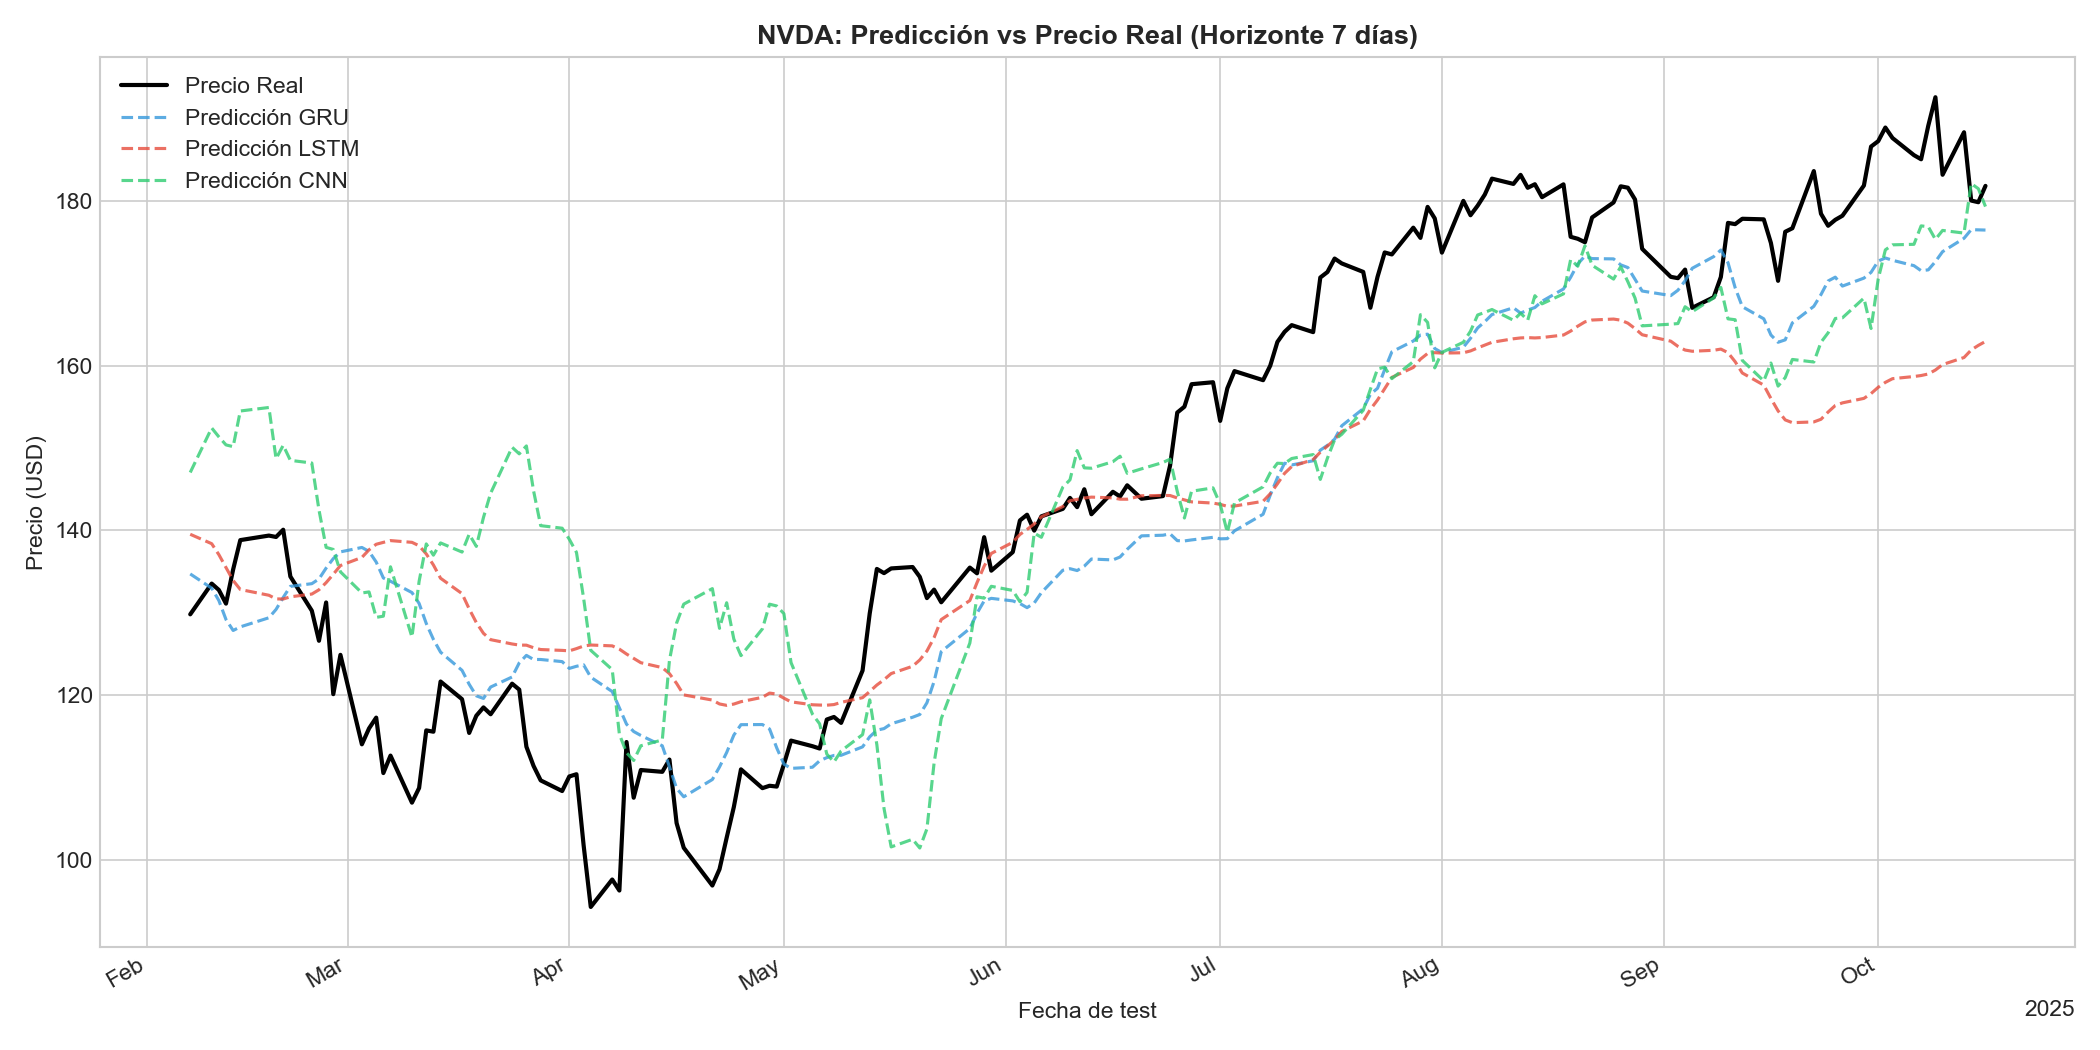
\includegraphics[width=0.95\textwidth]{Imagenes/pred_vs_actual_NVDA_h7.png}
\caption{NVDA: Predicción vs Real (7 días). A una semana, el modelo mantiene la dirección general pero pierde precisión en los puntos de inflexión. Los periodos de alta volatilidad ---especialmente durante noticias sobre IA--- presentan mayor error.}
\label{fig:pred_nvda_h7}
\end{figure}

\begin{figure}[H]
\centering
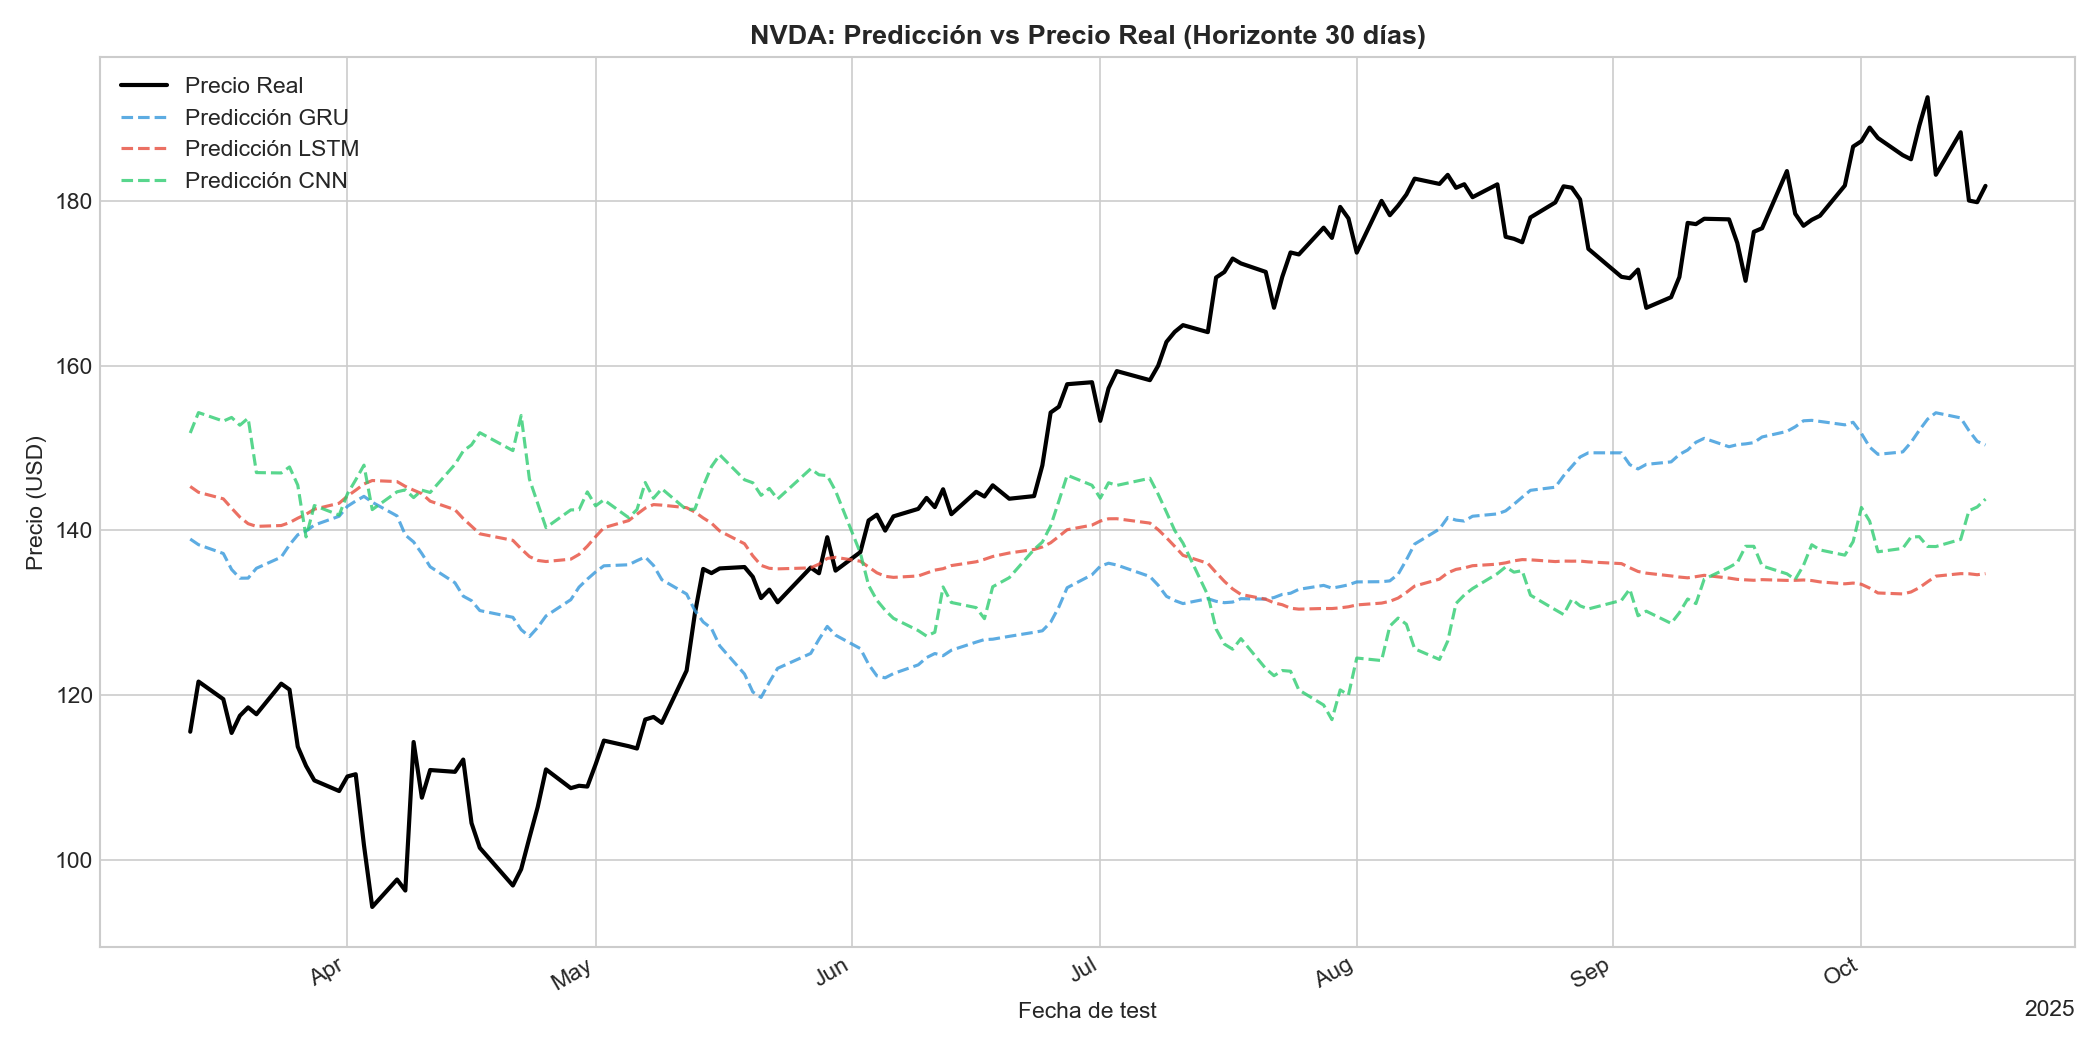
\includegraphics[width=0.95\textwidth]{Imagenes/pred_vs_actual_NVDA_h30.png}
\caption{NVDA: Predicción vs Real (30 días). Con horizonte mensual, la predicción captura movimientos de medio plazo pero falla en anticipar cambios de ritmo. La fuerte tendencia alcista del periodo analizado ayuda a que las predicciones sean razonables en términos de dirección.}
\label{fig:pred_nvda_h30}
\end{figure}

En Nvidia, las curvas muestran un seguimiento razonable de la tendencia, aunque con errores notables en los cambios de ritmo. Al ser el activo más vinculado al boom de la inteligencia artificial, su precio está fuertemente influenciado por noticias y expectativas del sector, lo que genera cambios de régimen difíciles de capturar. La lectura general es similar a la de los otros activos: existe estructura temporal aprovechable, pero la volatilidad y los eventos externos limitan la capacidad predictiva del modelo.

%% ============================================================
%% RESUMEN VISUAL
%% ============================================================

\clearpage
\section{Resumen visual}

Esta sección consolida los hallazgos principales mediante visualizaciones de síntesis. Aunque no añaden resultados nuevos, estas figuras facilitan la comparación de patrones y la comprensión global de los experimentos realizados.

\begin{figure}[H]
\centering
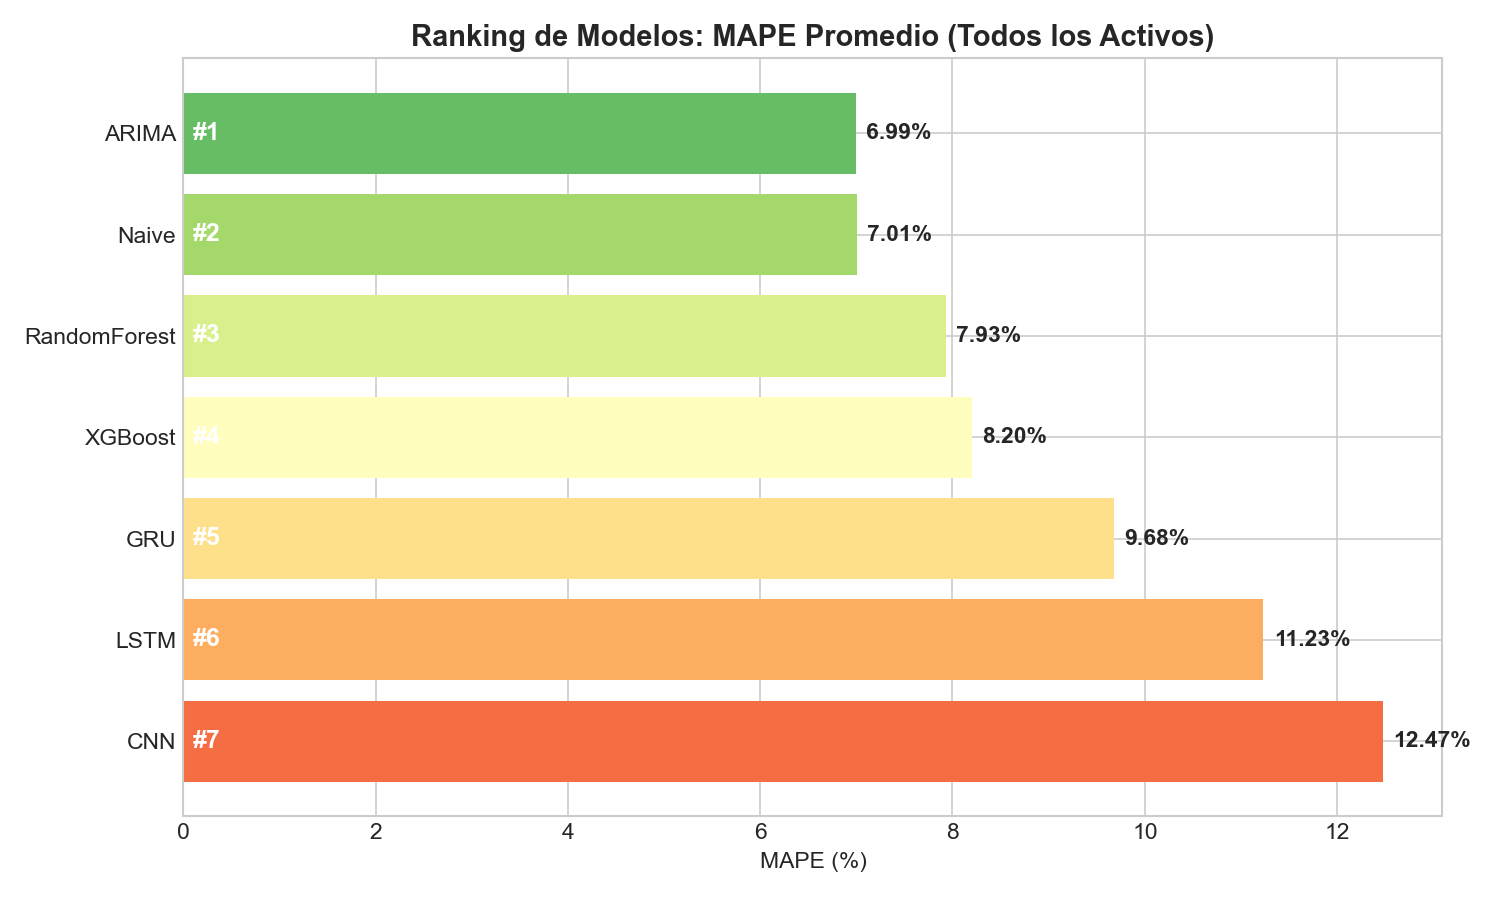
\includegraphics[width=0.90\textwidth]{Imagenes/summary_model_ranking.png}
\caption{Ranking global de modelos.}
\label{fig:summary_ranking}
\end{figure}

La Figura~\ref{fig:summary_ranking} presenta el ranking consolidado de los siete modelos evaluados. Se observa que los baselines (Naive y ARIMA) lideran el rendimiento medio, con los modelos de árboles a cierta distancia; las arquitecturas de aprendizaje profundo quedan en la parte baja del ranking. Esta visualización permite identificar rápidamente qué familias de modelos se acercan a los baselines y cuáles no justifican su complejidad adicional en esta configuración experimental.

\begin{figure}[H]
\centering
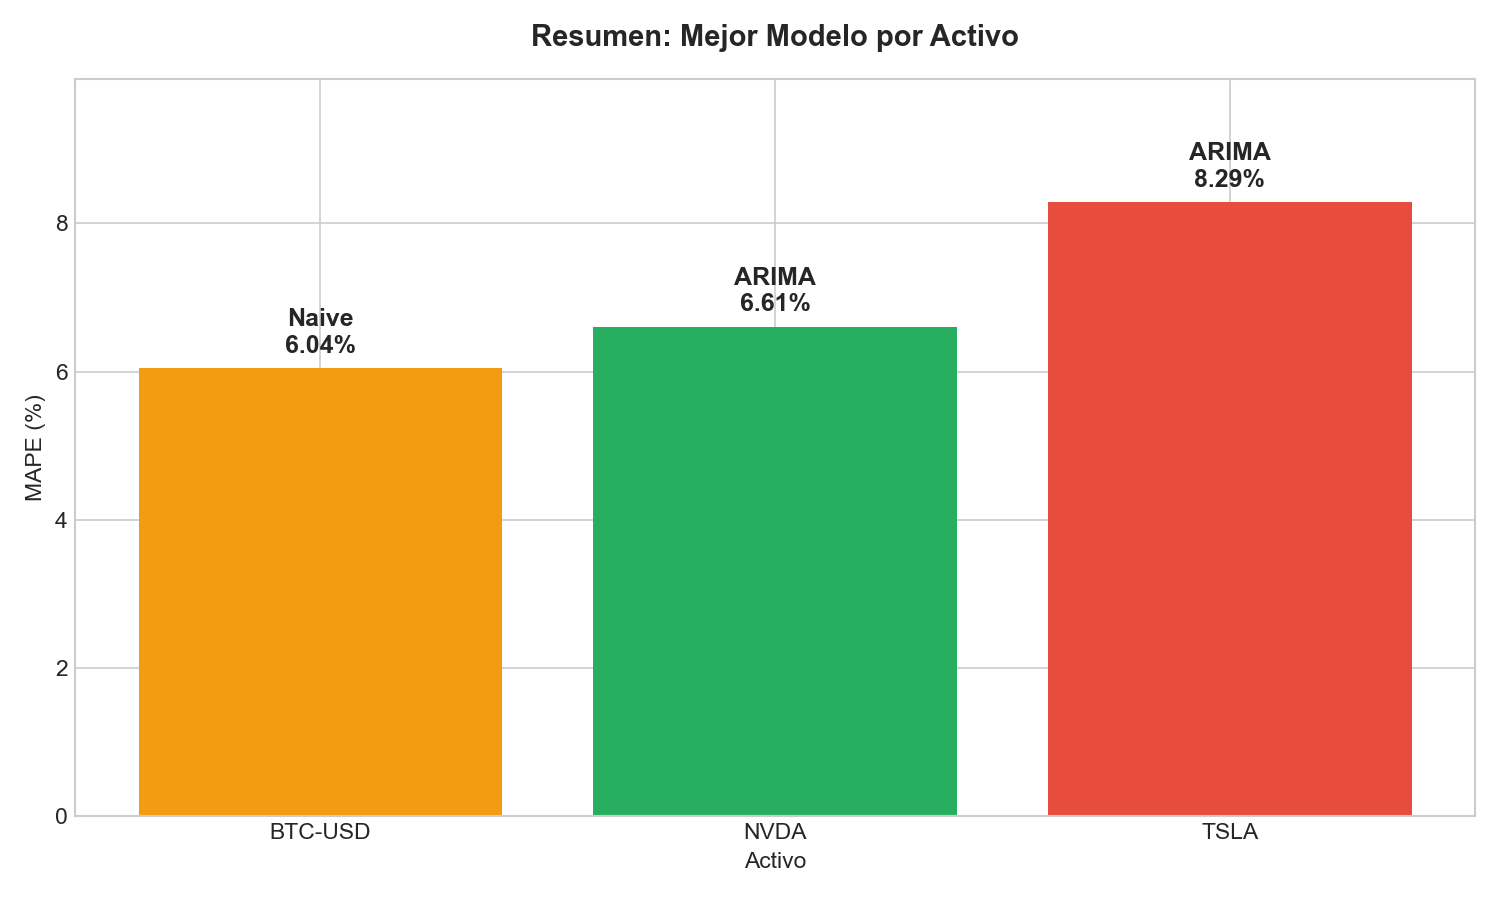
\includegraphics[width=0.85\textwidth]{Imagenes/summary_best_models.png}
\caption{Mejor modelo por activo.}
\label{fig:summary_best}
\end{figure}

La Figura~\ref{fig:summary_best} desglosa el mejor modelo para cada activo analizado. En este experimento, Naive es el mejor en BTC-USD, mientras que ARIMA lidera en TSLA y NVDA. Esta heterogeneidad refuerza la importancia de evaluar cada combinación modelo-activo de forma independiente.

\begin{figure}[H]
\centering
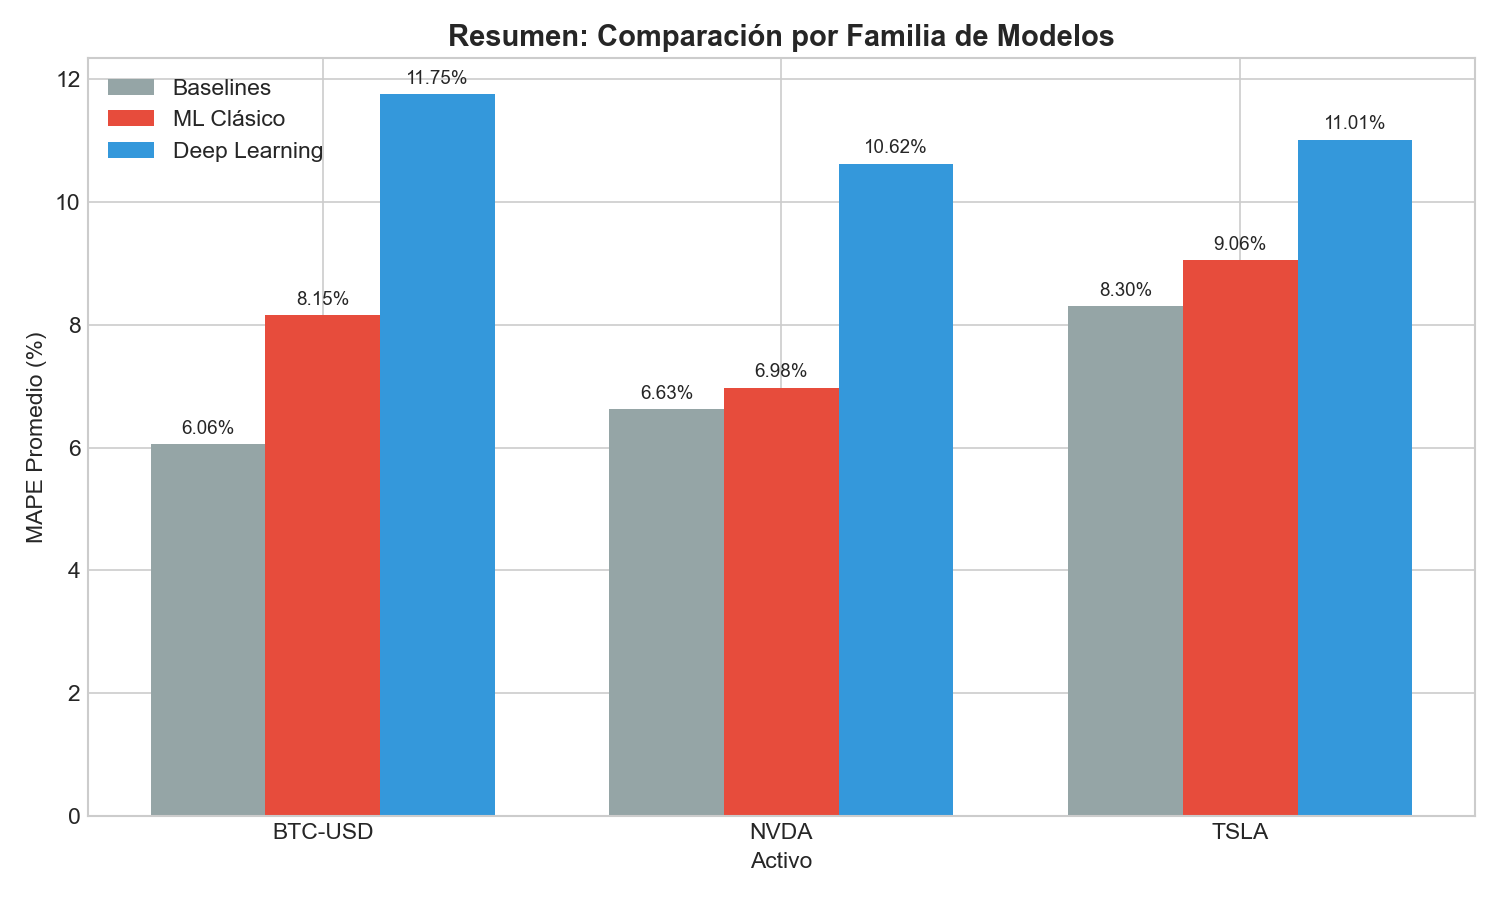
\includegraphics[width=0.90\textwidth]{Imagenes/summary_dl_vs_baselines.png}
\caption{Deep Learning vs Baselines.}
\label{fig:summary_dl_baselines}
\end{figure}

La Figura~\ref{fig:summary_dl_baselines} compara directamente los modelos de deep learning contra los baselines (Naive y ARIMA). Esta comparación es fundamental para responder a la pregunta de si la complejidad del deep learning aporta valor real. En estos resultados, los modelos DL no superan a los baselines en ninguno de los activos y presentan errores sustancialmente mayores, lo que sugiere que, con esta configuración, el valor añadido del deep learning no se materializa.

\begin{figure}[H]
\centering
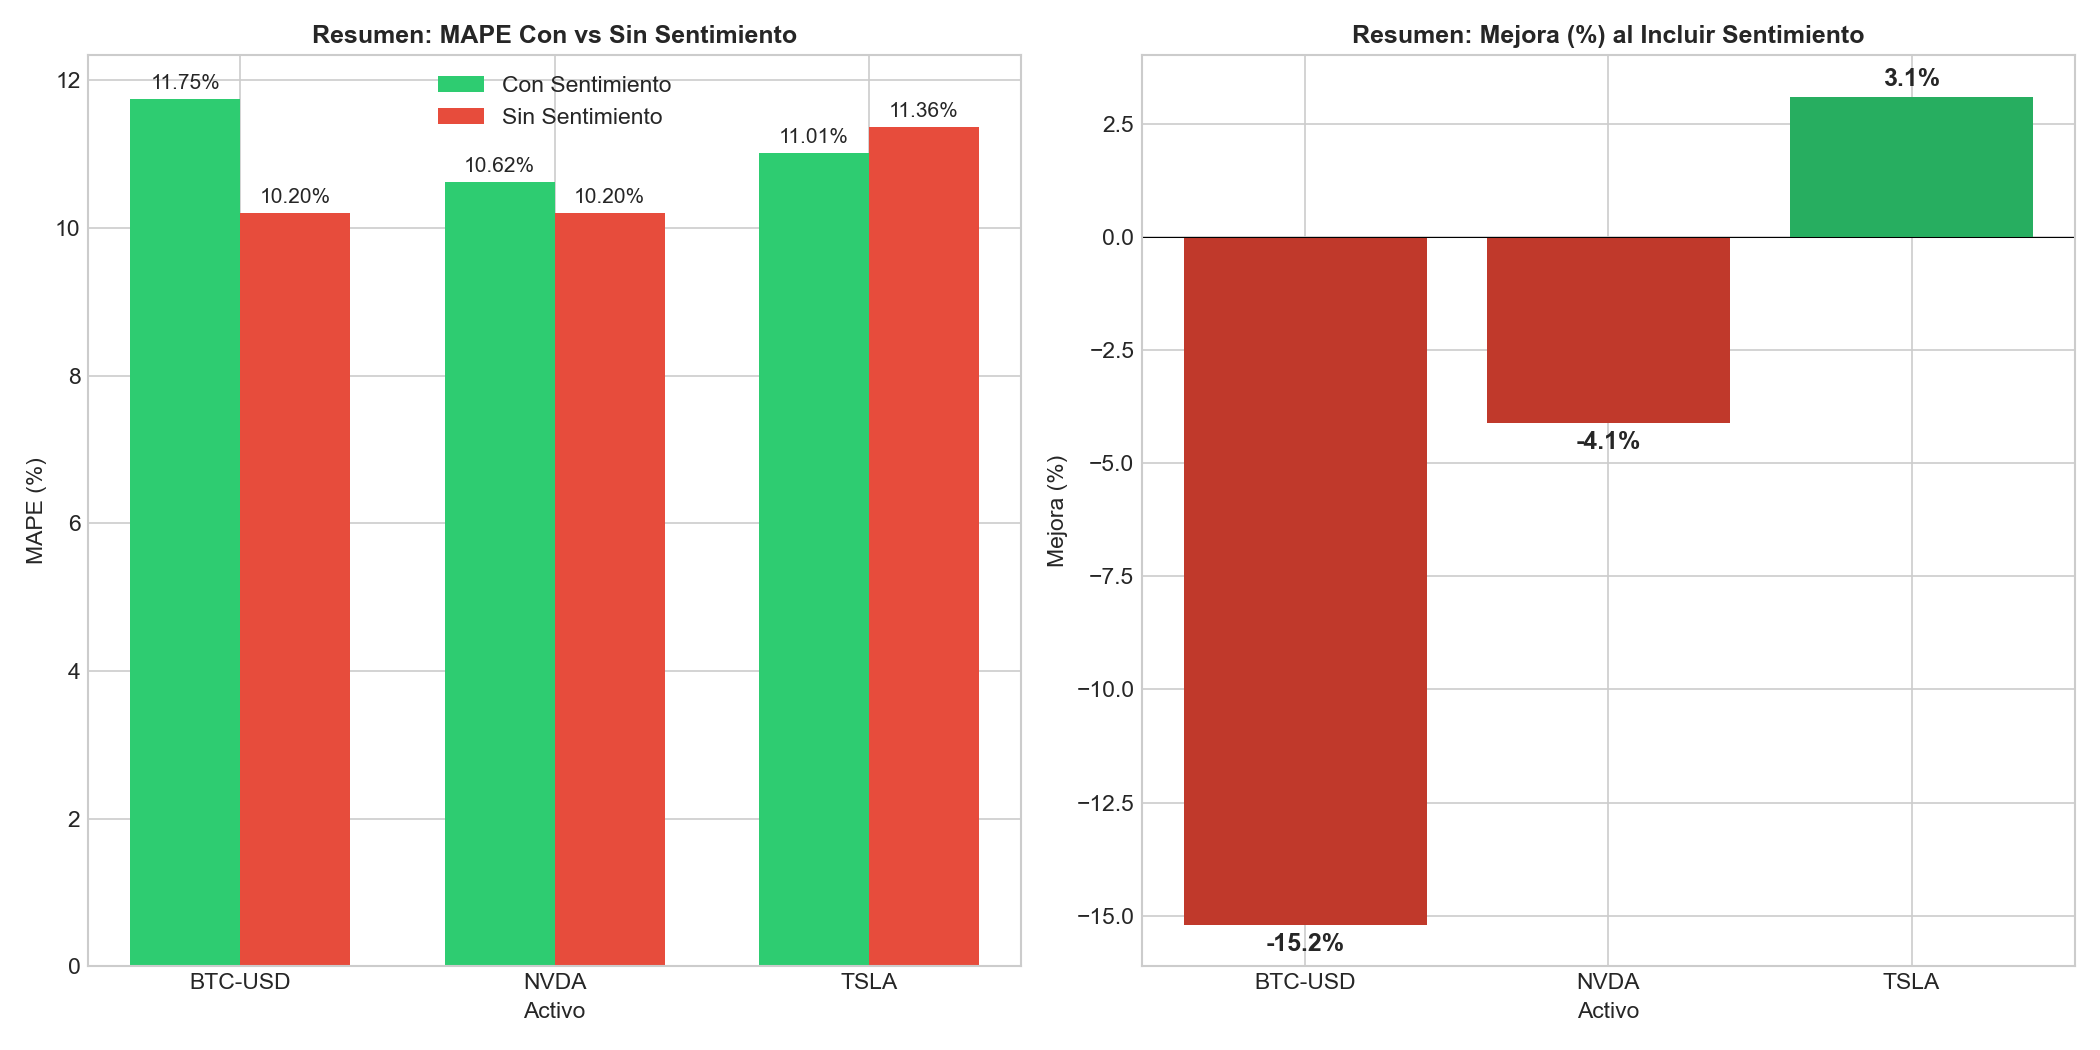
\includegraphics[width=0.95\textwidth]{Imagenes/summary_sentiment_impact.png}
\caption{Impacto del sentimiento.}
\label{fig:summary_sentiment}
\end{figure}

La Figura~\ref{fig:summary_sentiment} resume el impacto del sentimiento en las predicciones. El gráfico muestra que el efecto del sentimiento es heterogéneo: en Tesla tiende a mejorar ligeramente las predicciones, en Bitcoin tiende a perjudicar y en Nvidia solo LSTM se beneficia de forma leve. Esta visualización sintetiza el hallazgo principal del estudio de ablación: el sentimiento no es una mejora universal, sino que su utilidad depende de la combinación específica de modelo y activo.

\begin{figure}[H]
\centering
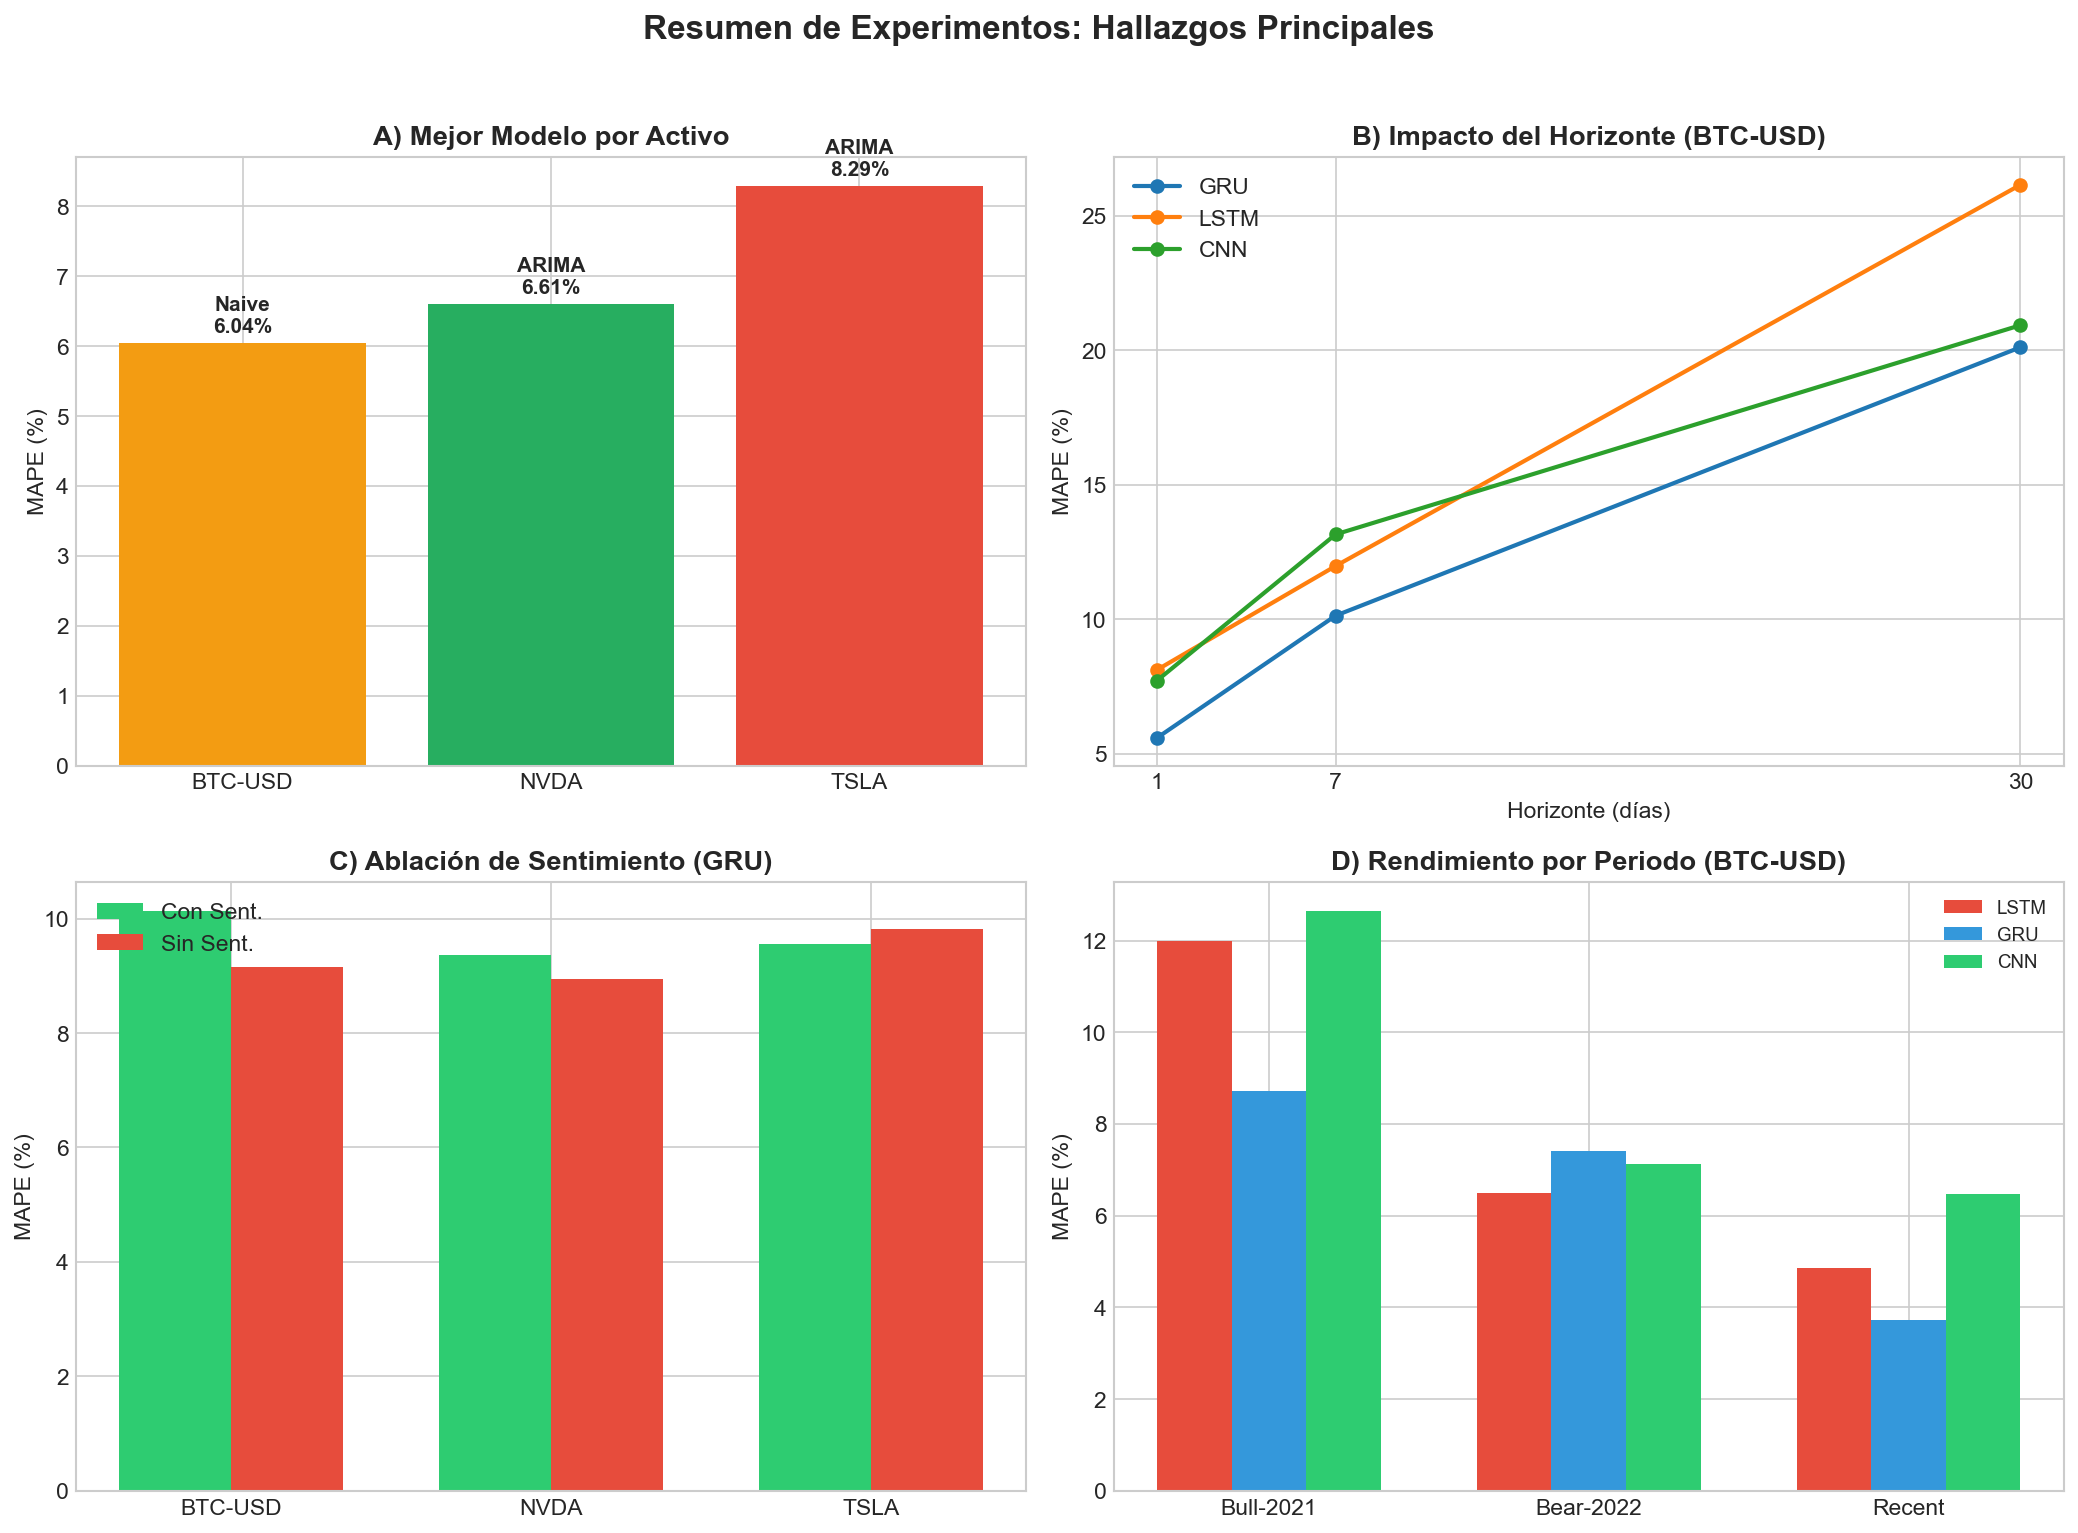
\includegraphics[width=0.95\textwidth]{Imagenes/summary_all_experiments.png}
\caption{Panel resumen de los cuatro experimentos.}
\label{fig:summary_all}
\end{figure}

Finalmente, la Figura~\ref{fig:summary_all} ofrece un panel que junta los cuatro experimentos (A: modelos, B: horizonte, C: ablación, D: periodos). Es la vista de pájaro del trabajo entero y ayuda a cruzar patrones que viendo cada experimento por separado podrían pasar desapercibidos.

\section{Lecciones extraídas de los datos}

Tras las figuras y tablas presentadas, estas son las conclusiones que los datos respaldan con cierta solidez:

\textbf{Los baselines dominan el MAPE.} ARIMA obtiene el mejor MAPE medio y Naive queda muy cerca; por activo, Naive lidera en BTC-USD y ARIMA en TSLA/NVDA. En esta configuración experimental, los modelos más complejos no mejoran esos baselines.

\textbf{CNN es el peor; los árboles no son competitivos.} CNN es sistemáticamente el modelo con mayor error. Random Forest y XGBoost quedan por detrás de Naive/ARIMA en los tres activos y, en BTC-USD, el test de Diebold-Mariano detecta empeoramiento significativo frente a Naive.

\textbf{GRU domina todos los horizontes en BTC.} A 1, 7 y 30 días mantiene el menor MAPE; LSTM queda por detrás y CNN se degrada al alargar el horizonte.

\textbf{La direccionalidad no muestra una ventaja robusta.} La precisión direccional se mueve típicamente en rangos cercanos al azar (aprox.\ 27--57\% según activo y modelo). Además, el baseline Naive genera una predicción ``plana'' y por eso su F1 direccional es 0, lo que ilustra que DA debe interpretarse junto con F1/MCC y el balance de clases.

\textbf{El sentimiento tiene un efecto pequeño y heterogéneo.} Mejora Tesla en los tres modelos y en NVDA solo con LSTM; empeora Bitcoin en los tres modelos y empeora también NVDA en CNN/GRU. En MAPE y DA/F1 no hay diferencias significativas según Wilcoxon (solo aparece un caso aislado en MCC).

\textbf{El rendimiento cambia por periodo, sin una regla simple.} En BTC-USD, GRU obtiene el mejor MAPE en el periodo reciente (3.71\%) y el peor en Bull-2021 (8.71\%). LSTM y CNN muestran una tendencia similar, pero el ranking entre ellos varía según el régimen: LSTM destaca en Bear-2022 y GRU en Bull-2021 y el periodo reciente. Conviene replicar con más particiones para confirmar estos patrones.

%% ============================================================
%% DISCUSIÓN CRÍTICA
%% ============================================================

\section{Discusión crítica: lo que los números no dicen}

Las tablas y gráficas presentan los datos de forma clara, pero conviene no sobreinterpretar un MAPE aparentemente bajo o unas curvas que parecen seguir la serie real. Un error bajo no significa utilidad práctica, y unas predicciones que ``parecen'' buenas visualmente pueden no aportar valor operativo si no superan tests estadísticos. En esta sección se ofrece una interpretación prudente de lo que los resultados sustentan y de sus limitaciones.

\subsection{Por qué los baselines dominan aquí}

En este esquema, Naive y ARIMA dominan de forma clara en MAPE en los tres activos. Una lectura plausible es que, para precios diarios y horizontes cortos, el cierre se comporta de forma cercana a un paseo aleatorio: la persistencia (``mañana parecido a hoy'') es muy difícil de batir. Cuando las señales adicionales (indicadores técnicos + sentimiento agregado) no aportan una ventaja estable, los modelos más complejos tienden a aprender ruido y a generalizar peor. El test de Diebold-Mariano refuerza esta lectura: no aparecen mejoras significativas frente a Naive y sí aparecen varios empeoramientos significativos.

\subsection{Interpretación realista del error}

Un MAPE de un solo dígito puede parecer reducido, pero conviene traducirlo a magnitudes absolutas para obtener una referencia de orden de magnitud.

\begin{itemize}
    \item BTC-USD: el mejor MAPE es $\sim$6\% y el precio medio del periodo ronda los 53.000 USD, así que el error medio está en torno a 3.200 USD.
    \item TSLA: el mejor MAPE es $\sim$8,3\% con precio medio cercano a 260 USD, lo que implica un error medio de unos 21 USD.
    \item NVDA: el mejor MAPE es $\sim$6,6\% con precio medio alrededor de 62 USD, lo que deja un error medio en torno a 4 USD.
\end{itemize}

Esto importa porque fija el orden de magnitud: si una estrategia no puede absorber errores de ese tamaño (más comisiones y spreads), la predicción deja de ser útil aunque el porcentaje parezca bajo.

Si quisiéramos usar estas predicciones para trading, tendríamos que considerar:

\textbf{Costes de transacción.} Entre spreads, comisiones y slippage, cada operación tiene un coste. Si el beneficio esperado es menor que el coste, la estrategia pierde dinero.

\textbf{Gestión del riesgo.} Un error medio del 5\% implica una distribución con valores más altos en determinados episodios (por ejemplo, 8\% o 12\%). La exposición y el tamaño de posición deberían ser coherentes con esa variabilidad.

\textbf{Frecuencia de operación.} Predicciones a 7 días implican pocas operaciones al año. Los beneficios tendrían que ser sustanciales para compensar el capital inmovilizado.

No se ha realizado un backtesting riguroso con costes reales; no obstante, es razonable anticipar que un MAPE moderado puede ser insuficiente para generar beneficios consistentes una vez incorporados costes de transacción y fricciones. Además, incluso cuando una curva de predicción aparenta seguir la serie real, ello no implica ventaja operativa ni superioridad estadística frente a un baseline.

\subsection{Precisión direccional: la métrica que importa}

En contextos de decisión, además del error absoluto, resulta relevante anticipar si el precio subirá o bajará. Para ello se utiliza la \textbf{precisión direccional}, definida como el porcentaje de veces que el modelo acierta la dirección del movimiento.

Se calcularon estas métricas para todos los modelos. La Tabla~\ref{tab:directional_accuracy} resume acierto direccional, F1 y MCC.

\begin{table}[H]
\centering
\caption{Métricas direccionales por modelo y activo}
\label{tab:directional_accuracy}
\begin{tabular}{l|ccc|c}
\hline
\textbf{Modelo/Metrica} & \textbf{BTC-USD} & \textbf{TSLA} & \textbf{NVDA} & \textbf{Media} \\
\hline
Naive - DA (\%) & 50.28 & 53.89 & 26.94 & 43.70 \\
Naive - F1 dir. (\%) & 0.00 & 0.00 & 0.00 & 0.00 \\
Naive - MCC & 0.00 & 0.00 & 0.00 & 0.00 \\
ARIMA - DA (\%) & 46.39 & 50.00 & 56.94 & 51.11 \\
ARIMA - F1 dir. (\%) & 41.97 & 44.91 & 64.46 & 50.45 \\
ARIMA - MCC & -0.16 & 0.06 & 0.02 & -0.03 \\
RandomForest - DA (\%) & 46.39 & 47.78 & 54.44 & 49.54 \\
RandomForest - F1 dir. (\%) & 39.40 & 36.59 & 53.29 & 43.09 \\
RandomForest - MCC & -0.00 & 0.02 & 0.13 & 0.05 \\
XGBoost - DA (\%) & 47.22 & 48.89 & 53.06 & 49.72 \\
XGBoost - F1 dir. (\%) & 42.23 & 32.30 & 51.04 & 41.86 \\
XGBoost - MCC & 0.05 & -0.06 & 0.16 & 0.05 \\
CNN - DA (\%) & 45.56 & 47.22 & 39.72 & 44.17 \\
CNN - F1 dir. (\%) & 34.39 & 43.45 & 32.55 & 36.80 \\
CNN - MCC & 0.07 & 0.09 & -0.04 & 0.04 \\
LSTM - DA (\%) & 46.39 & 55.83 & 39.17 & 47.13 \\
LSTM - F1 dir. (\%) & 42.34 & 46.43 & 36.68 & 41.82 \\
LSTM - MCC & 0.05 & 0.17 & 0.08 & 0.10 \\
GRU - DA (\%) & 46.94 & 55.56 & 43.33 & 48.61 \\
GRU - F1 dir. (\%) & 41.78 & 36.76 & 38.38 & 38.98 \\
GRU - MCC & 0.01 & 0.08 & 0.11 & 0.07 \\
\hline
\end{tabular}
\end{table}

Los resultados muestran heterogeneidad. La dirección se comporta de forma distinta a los errores absolutos: hay activos donde algunos modelos aciertan más la dirección aun sin ser los mejores en MAPE, y viceversa. Esto refuerza que las métricas direccionales son sensibles al periodo de test y al activo, y deben leerse con cautela. Por tanto, la selección del ``mejor modelo'' depende de la métrica objetivo.

En este protocolo se obtienen 360 predicciones en el test por activo. La mayoría de modelos se sitúan en torno al 50\% de precisión direccional y, aunque existen diferencias entre activos, no aparece una ventaja direccional grande y estable. Además, el baseline Naive produce un cambio predicho igual a 0 (predicción plana), por lo que su F1 direccional es 0; esto recuerda que la DA debe interpretarse junto con F1/MCC y el balance de clases.

Conviene matizar, sin embargo, que un acierto direccional elevado no implica necesariamente utilidad económica. Si los errores se concentran en jornadas con movimientos grandes, su impacto puede superar el de múltiples aciertos en jornadas con movimientos pequeños. Además, con ventanas de test relativamente cortas, estas proporciones pueden verse afectadas por variabilidad muestral. La Figura~\ref{fig:directional_accuracy} visualiza estos resultados.

\begin{figure}[H]
\centering
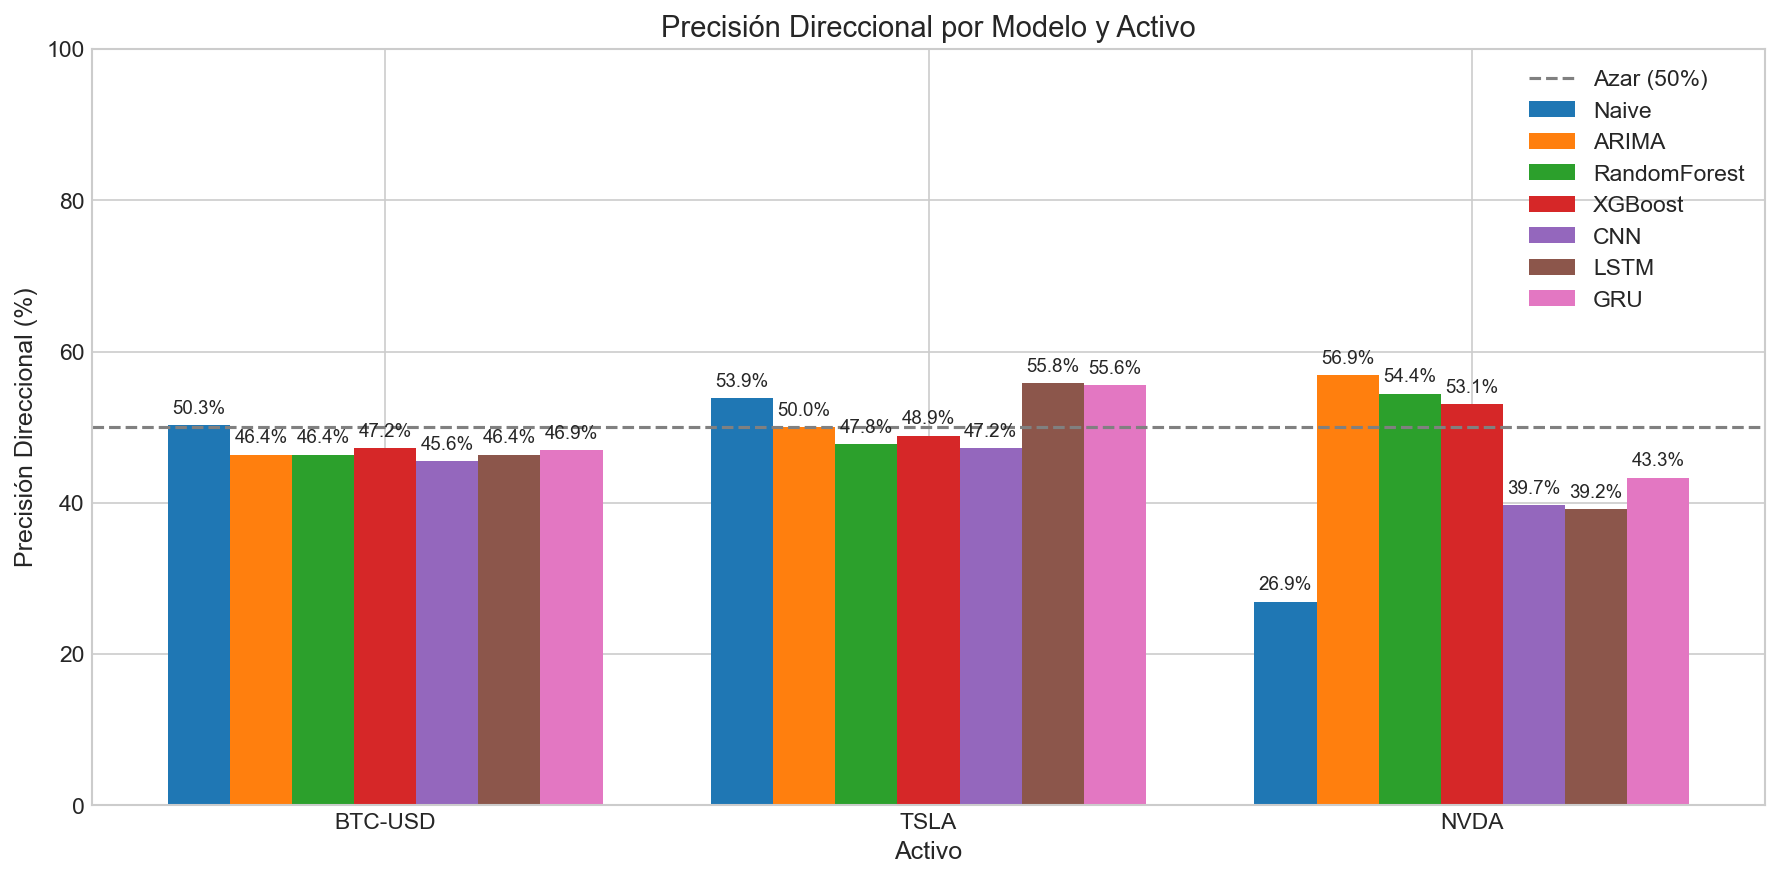
\includegraphics[width=0.95\textwidth]{Imagenes/directional_accuracy_comparison.png}
\caption{Precisión direccional por modelo y activo. La línea discontinua marca el 50\% (azar).}
\label{fig:directional_accuracy}
\end{figure}

\subsection{Significancia estadística de las diferencias}

La cuestión relevante es si un modelo mejora realmente a Naive o si la diferencia podría explicarse por ruido muestral. El \textbf{test de Diebold-Mariano}~\cite{diebold1995comparing} permite responder formalmente a esta pregunta comparando los errores de dos modelos. En este trabajo se ejecuta con horizonte 7, igual que el horizonte de predicción principal.

La Tabla~\ref{tab:diebold_mariano} muestra los resultados del test para cada activo y modelo comparado contra Naive.

\begin{table}[H]
\centering
\caption{Test de Diebold-Mariano: Naive vs cada modelo}
\label{tab:diebold_mariano}
\begin{tabular}{l|l|ccc}
\hline
\textbf{Activo} & \textbf{Modelo} & \textbf{Estadistico DM} & \textbf{p-value} & \textbf{Significativo?} \\
\hline
BTC-USD & ARIMA & -0.41 & 0.682 & No \\
BTC-USD & CNN & 3.52 & 0.000 & Si \\
BTC-USD & GRU & 2.63 & 0.009 & Si \\
BTC-USD & LSTM & 2.69 & 0.007 & Si \\
BTC-USD & RandomForest & 2.21 & 0.028 & Si \\
BTC-USD & XGBoost & 2.71 & 0.007 & Si \\
NVDA & ARIMA & -0.58 & 0.565 & No \\
NVDA & CNN & 2.81 & 0.005 & Si \\
NVDA & GRU & 2.48 & 0.014 & Si \\
NVDA & LSTM & 2.77 & 0.006 & Si \\
NVDA & RandomForest & -1.23 & 0.220 & No \\
NVDA & XGBoost & -0.69 & 0.489 & No \\
TSLA & ARIMA & 0.31 & 0.754 & No \\
TSLA & CNN & 2.75 & 0.006 & Si \\
TSLA & GRU & 1.50 & 0.135 & No \\
TSLA & LSTM & 1.63 & 0.103 & No \\
TSLA & RandomForest & 1.03 & 0.302 & No \\
TSLA & XGBoost & 0.93 & 0.351 & No \\
\hline
\end{tabular}
\end{table}

La Figura~\ref{fig:dm_pvalues} resume los p-values del test frente a Naive y permite apreciar que no aparecen mejoras robustas.

\begin{figure}[H]
\centering
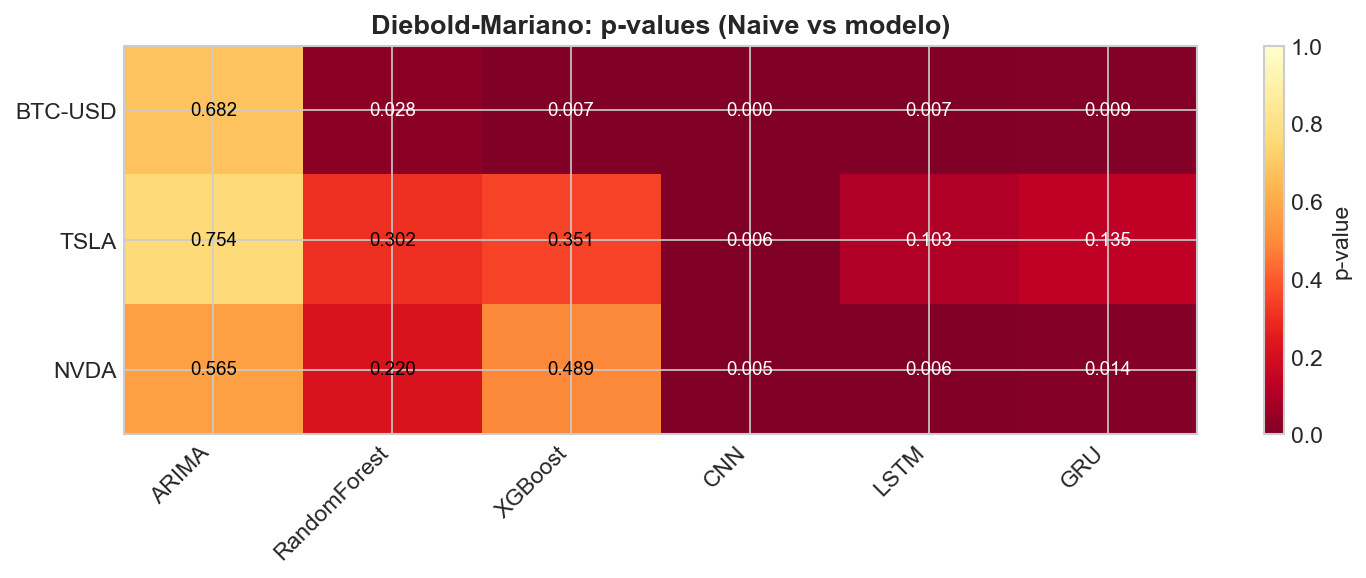
\includegraphics[width=0.90\textwidth]{Imagenes/diebold_mariano_pvalues_heatmap.png}
\caption{P-values del test de Diebold-Mariano (Naive vs cada modelo).}
\label{fig:dm_pvalues}
\end{figure}

Los resultados muestran dos hechos: (1) no hay evidencia de que ningún modelo mejore significativamente a Naive; y (2) sí aparecen empeoramientos significativos en varias comparaciones (especialmente CNN/LSTM/GRU en BTC-USD y NVDA, CNN en TSLA, y también Random Forest/XGBoost en BTC-USD). ARIMA, por su parte, no difiere significativamente de Naive.

\subsection{Limitación clave: eventos externos}

Una limitación estructural de este enfoque es que los modelos se entrenan con información observable en el histórico (precio, indicadores y sentimiento agregado). Sin embargo, eventos externos (anuncios corporativos, cambios regulatorios, noticias inesperadas) pueden provocar movimientos abruptos que no están reflejados de forma directa en las variables de entrada. En esos casos, el error aumenta para todos los modelos, independientemente de su complejidad.

Por tanto, lo máximo que puede esperarse de estos modelos es capturar la componente relativamente estable y repetible de la dinámica del precio. Esto ayuda a explicar por qué el rendimiento tiende a degradarse en fases de alta incertidumbre o cambios de régimen: cuando aumenta el peso de los shocks, la parte ``predecible'' se reduce.

\begin{figure}[H]
\centering
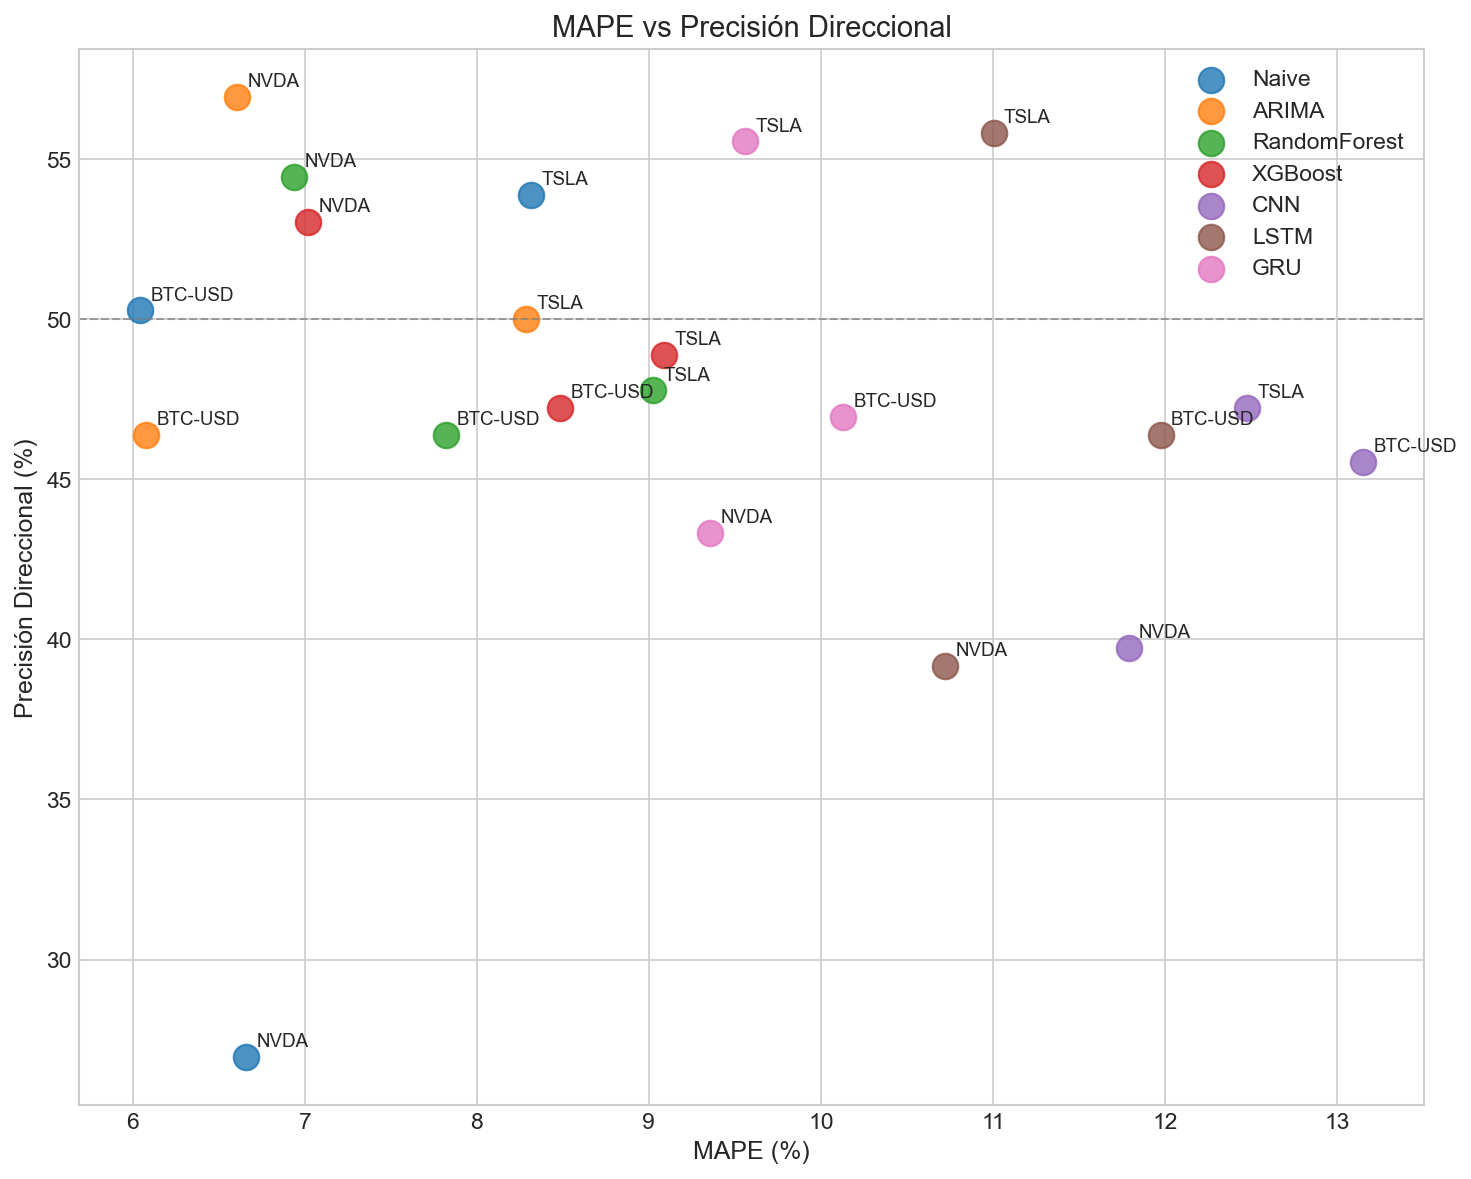
\includegraphics[width=0.90\textwidth]{Imagenes/mape_vs_directional_accuracy.png}
\caption{Relación entre MAPE y Precisión Direccional. Nótese que un MAPE bajo no siempre implica alta precisión direccional.}
\label{fig:mape_vs_da}
\end{figure}

La Figura~\ref{fig:mape_vs_da} muestra la relación entre MAPE y precisión direccional. Curiosamente, no hay una correlación perfecta: algunos modelos con MAPE similar tienen precisiones direccionales muy diferentes. Esto refuerza la idea de que ambas métricas capturan aspectos distintos del rendimiento predictivo.
